\documentclass[fleqn]{rbfin}

%%%%%%%%%%%%%%%%%%%%%%%%%%%%%%%%%%%%
% COPYDESK INFO (DON'T WORRY ABOUT THESE)
%%%%%%%%%%%%%%%%%%%%%%%%%%%%%%%%%%%%
%\usepackage{draftwatermark}
%\SetWatermarkAngle{45}
%\SetWatermarkLightness{.92}
%\SetWatermarkFontSize{20pt}
%\SetWatermarkScale{6}
%\SetWatermarkText{\sf{Manuscript}}

\def\rbfinsubmitted{}
\def\rbfinaccepted{}
\def\rbfinpublished{}
\def\rbfineditor{}
\def\rbfinDOI{10.xxxx/xxxx}

\def\rbfinyear{2026}
\def\rbfinvolume{}
\def\rbfinpages{}
\pagina{1}
%%%%%%%%%%%%%%%%%%%%%%%%%%%%%%%%%%%%

%%%%%%%%%%%%%%%%%%%%%%%%%%%%%%%%%%%%
% CUSTOM PACKAGES
% (LOAD CUSTOM PACKAGES BELOW)
%%%%%%%%%%%%%%%%%%%%%%%%%%%%%%%%%%%%
% \usepackage{tikz}

%%%%%%%%%%%%%%%%%%%%%%%%%%%%%%%%%%%%
% BEGIN DOCUMENT
%%%%%%%%%%%%%%%%%%%%%%%%%%%%%%%%%%%%
\begin{document}
% SELECT ARTICLE LANGUAGE
% Para artigos em PORTUGUÊS, alterar a linha abaixo para \selectlanguage{brazilian}
\selectlanguage{english}
\frenchspacing

%%%%%%%%%%%%%%%%%%%%%%%%%%%%%%%%%%%%
% FRONT MATTER
%%%%%%%%%%%%%%%%%%%%%%%%%%%%%%%%%%%%

% ARTICLE TITLE
\title{Hybrid Centrality and Network Topology in Equity Markets: Asset Pricing and Portfolio Implications} % Appears on title page

% ARTICLE SHORT TITLE
\shorttitle{Hybrid Centrality and Network Topology in Equity Markets: Asset Pricing and Portfolio Implications} % appears on header every other page

%%%%%%%%%%%%%%%%%%%%%%%%%%%%%%%%%%%%
% AUTHOR INFORMATION
%%%%%%%%%%%%%%%%%%%%%%%%%%%%%%%%%%%%
\author{\centering
% Define affiliations
\affiliations{1}{Instituto de Ciências Exatas, Universidade Federal de Juiz de Fora, Juiz de Fora, Brazil}
\affiliations{2}{FGV Escola de Economia de São Paulo, Fundação Getulio Vargas, São Paulo, Brazil}
\affiliations{3}{Faculdade Belavista, Departamento de Economia, São Paulo, Brazil}
% AUTHOR 1
\textbf{Gustavo Ribeiro de Oliveira Roque}%
\email{gustavo.roque@estudante.ufjf.br}
\affiliationlink{1} % Match with the affiliations defined above
\orcidlink{0009-0002-5203-3480}
\and % separate authors with \and
% AUTHOR 2
\textbf{Maurício Ferraresi}%
\email{mauricio.ferraresi@fgv.br}
\affiliationlink{2} % Match with the affiliations defined above
\affiliationlink{3} % Match with the affiliations defined above
\orcidlink{0000-0001-6600-6403}
\and
% AUTHOR 3
\textbf{Carlos Cristiano Hasenclever Borges}%
\email{carlos.cristiano@ufjf.br}
\affiliationlink{1} % Match with the affiliations defined above
\orcidlink{0000-0001-7413-2880}
% AND SO ON...
\\[11pt]
% Print the affiliations:
\affiliationname{1}
\affiliationname{2}
\affiliationname{3}
}
\autorlong{Roque et al., \rbfinyear} % appears on header every other page
%\autorlong{One, A., Two, A. \& Three, A. (\rbfinyear{})} % only affects the “how-to-cite” text.
\maketitle

% ABSTRACT, KEYWORDS AND JEL
\begin{abstract}
\myabstract{%
This paper investigates whether information diffusion dynamics in equity markets are associated with the topology of correlation-based financial networks. Using a rolling-window approach from 2014 to 2024, we construct financial networks via the Triangulated Maximally Filtered Graph (TMFG) and introduce a Hybrid Centrality Metric (HCM) that aggregates degree, eigenvector, and closeness centralities to decompose the investment universe into core and peripheral portfolios. Fama-French three-factor regressions reveal a monotonic deterioration in systematic market integration from the core to the periphery: the central portfolio behaves as a high-beta market conduit with negative alpha, whereas the peripheral portfolio attenuates this footprint and generates positive alpha. A cross-sectional test shows that roughly 62\% of the variation in HCM is orthogonal to beta, size, and momentum, supporting its interpretation as a descriptive topological dimension that is correlated with, but not reducible to, firm size. The peripheral alpha survives multiple-testing corrections (Holm--Bonferroni $p=0.034$; reality-check $p=0.006$), but it is concentrated in small caps, is partly explained by a betting-against-beta effect, and weakens substantially once non-stock vehicles are excluded. In-sample, the central core systematically leads the periphery and the network signal dominates the traditional size-based effect; out-of-sample, however, the size effect is the more resilient predictor and the network signal falls below it, so we report this degradation explicitly rather than overstate predictability. Backtests of the peripheral and opposing combination strategies still deliver strong risk-adjusted returns and favorable drawdown mitigation relative to the market. These results indicate that financial network topology provides an actionable, economically interpretable framework for quantitative portfolio management, while highlighting the limits of network-based lead--lag predictability out of sample.
}

% KEYWORDS (separated by semicolon)
\keywordslist{Financial networks; Correlation matrix; TMFG; Centrality; Lead--lag effects; Return predictability.}

% JEL CODES (separated by comma)
\jelcodeslist{G12, C58, C63, C32.}
\end{abstract}

%%%%%%%%%%%%%%%%%%%%%%%%%%%%%%%%%%%%
% END OF FRONT MATTER
%%%%%%%%%%%%%%%%%%%%%%%%%%%%%%%%%%%%

%%%%%%%%%%%%%%%%%%%%%%%%%%%%%%%%%%%%
% DOCUMENT MAIN SECTIONS
%%%%%%%%%%%%%%%%%%%%%%%%%%%%%%%%%%%%

\section{Introduction}

\noindent Understanding how information diffuses across financial markets remains a central question in asset pricing and portfolio management. While individual stock returns typically exhibit negligible auto-correlation, portfolios often display significant positive autocorrelation over time. This phenomenon, recently documented by \citet{li2022detecting}, implies the presence of robust cross-autocorrelations in which the returns of some stocks systematically lead those of others. Identifying and exploiting such lead--lag relationships has therefore become an important research direction, both for understanding market microstructure and for designing resilient trading strategies.

In this paper, we investigate whether these information diffusion dynamics are associated with the topology of correlation-based financial networks. Rather than identifying market leaders and followers using predefined, traditional firm characteristics, such as market capitalization, sector membership, or momentum, we propose a network-driven decomposition of the investment universe. By extracting the structural backbone of market interactions, we test whether a stock's topological centrality within a filtered system of global dependencies is associated with its role in lead--lag relationships and cross-sectional asset pricing. Because the centrality ranking is correlated with firm size and liquidity, we interpret it as a descriptive structural dimension and treat size, low-beta, and liquidity as candidate economic drivers in the robustness analysis.

To implement this framework, we construct robust correlation-based networks using a rolling-window approach from 2014 to 2024. Departing from traditional, static lookback periods, we utilize 5 years of past daily returns, dynamically smoothed via exponential weighting and stabilized using Ledoit-Wolf shrinkage \cite{ledoit2004honey}. This ensures our correlation matrices optimally balance recent structural innovations with historical stability. To filter these dense matrices, we employ the Triangulated Maximally Filtered Graph (TMFG) \cite{massara2016network}. Compared to alternative filtering techniques like the Minimum Spanning Tree (MST) or Planar Maximally Filtered Graph (PMFG), the TMFG retains a richer amount of local clustering information while remaining computationally scalable ($O(N^2)$) for high-dimensional financial datasets. Within these planar networks, we classify stocks into central (core) and peripheral portfolios. Crucially, we contrast a traditional centrality measure (the Pozzi metric \citet{pozzi2013spread}) against our novel Hybrid Centrality Metric (HCM), which aggregates degree, eigenvector, and closeness centralities to provide a more holistic view of a node's systemic importance.

Our methodology departs from the existing literature in two critical dimensions. First, building on the insights of \citet{pozzi2013spread}, who demonstrated that risk is not uniformly distributed across financial networks, we focus on strict topological centrality rather than recursive influence, adopting a more direct and economically interpretable construction to achieve a clearer topological separation between core and periphery. Second, unlike characteristic-based approaches that impose leadership hierarchies ex-ante, our leaders and followers emerge strictly from the data. This allows us to formulate testable hypotheses regarding how structural position dictates information diffusion, rather than merely developing algorithmic detection methods.

Empirically, our results demonstrate that network topology captures a distinct structural dimension of the equity market. The HCM framework reveals a stable market hierarchy, with annual decile-membership turnover clustering between 33\% and 65\%, contrasting with the Pozzi metric, which frequently exhibits membership turnover exceeding 75\%. The resulting network portfolios cannot be trivially explained by traditional risk factors.

Most importantly, this topological separation translates directly into asset pricing and directional predictability. Time-series Fama-French three-factor regressions reveal a monotonic deterioration in systematic market integration from the core to the periphery. Our novel metric successfully captures the differences between extremes: the central portfolio (Decile 1) acts as a high-beta systematic conduit with a Market Beta of $0.8915$ and an explanatory power of $R^2 = 0.9537$, alongside a significant negative alpha of $-0.0240$ ($t$-stat $=-2.2673$). Conversely, the HCM peripheral portfolio (Decile 10) attenuates this market footprint, falling to a Market Beta of $0.2808$ and an $R^2$ of $0.3562$, while generating a statistically significant positive alpha of $0.1013$ ($t$-stat $= 2.0682$). In comparison to Pozzi's metric, the monotonic decline from center to periphery is preserved, though with less pronounced separation: the central portfolio attains a Market Beta of $0.7816$ with an $R^2$ of $0.8617$ (indicating lower explanatory power), while the peripheral portfolio records a Market Beta of $0.5528$ and an $R^2$ of $0.5839$. 

To further test the economic viability of network-based positioning, we construct combination portfolios that equally weight symmetrically opposed deciles, blending structural extremes with intermediate groupings. Under our novel metric, the portfolio uniting center and periphery yields an annualized alpha of $0.0375$ ($t$-stat $= 1.3663$) with a market beta of $0.5785$ and an $R^2$ of $0.8131$. The Pozzi metric exhibits a similar behavior, yielding an annualized alpha of $0.0271$, a market beta of $0.6685$, and an $R^2$ of $0.8025$. Analyzing this combination of core and periphery is useful for traders seeking to exploit potential predictive relationships from central to peripheral assets.

Furthermore, we find evidence of a systematic in-sample lead--lag relationship: the central core rapidly absorbs market-wide information and systematically leads the peripheral portfolio within the estimation window, and this network-derived dependency dominates the traditional Big-leads-Small size effect. Out-of-sample, however, this advantage does not persist: the size-based effect re-emerges as the more resilient predictor and the network signal generally falls below it, occasionally turning negative. While our metric still outperforms the Pozzi metric out of sample, we report this degradation explicitly rather than overstate predictability; the more robust contribution of the framework is the topology-driven portfolio construction analyzed below.

To assess the investment viability of these network-based strategies, we backtest them over the sample period using an equally weighted buy-and-hold portfolio structure and compare their performance against an equal-weighted ($1/N$), buy-and-hold benchmark of the full network universe, which delivers a CAGR of $11.04\%$, an annualized volatility of $15.61\%$, and a Sharpe ratio of $0.75$. This benchmark is deliberately distinct from the capitalization-weighted market benchmark used in the Treynor--Black analysis of Section~\ref{sec:results}.\footnote{Two benchmarks are used throughout: an equal-weighted ($1/N$), buy-and-hold portfolio of the full network universe for the decile and combination portfolios, and a capitalization-weighted market portfolio as the passive benchmark in the Treynor--Black analysis. The two answer different questions and are not directly comparable.} The two yardsticks answer different questions and are therefore not directly comparable to one another. Under the Hybrid Centrality Metric (HCM) framework, the central portfolio (Decile 1) underperforms the broader market, achieving a CAGR of $8.40\%$ alongside an annualized volatility of $18.26\%$ and a Sharpe ratio of $0.53$ (with a Sortino ratio of $0.75$ and a Maximum Drawdown of $-34.36\%$). Conversely, the HCM peripheral portfolio (Decile 10) elevates performance to a CAGR of $15.12\%$ while suppressing risk to an annualized volatility of $12.20\%$. This combination yields strong risk-adjusted returns, with a Sharpe ratio of $1.22$ and a Sortino ratio of $1.66$. Furthermore, the HCM periphery demonstrates favorable tail-risk mitigation, restricting its Maximum Drawdown to $-30.69\%$ and registering a 99\% Value at Risk (VaR) of $-1.91\%$ and a Conditional Value at Risk (CVaR) of $-2.94\%$. The Pozzi metric exhibits a similarly profitable peripheral profile, yielding a $14.33\%$ CAGR and a $0.90$ Sharpe ratio for peripheral assets, though it lacks the pronounced volatility dampening observed in the HCM periphery. To balance core stability and peripheral return generation, we also examine symmetric combination strategies. Under the HCM framework, this combined strategy produces a CAGR of $11.96\%$ with a volatility of $13.14\%$, a Sharpe ratio of $0.93$, a Sortino ratio of $1.26$, and the smallest Maximum Drawdown in the sample at $-27.21\%$.

Building on these baseline characteristics, we translate this structural asymmetry into an actionable, institutional-grade investment strategy by extending our network analysis through a quantitative portfolio optimization framework. Leveraging the Sharpe (1963) Single-Index Model, we isolate the idiosyncratic alpha of the network extremes and optimize capital allocation using the Treynor-Black (1973) model. We evaluate both unconstrained and long-only mandates against a capitalization-weighted benchmark comprising the entire network universe, systematically allocating to peripheral stocks exhibiting positive alpha while hedging against the highly integrated central core.

Our out-of-sample backtests, computed net of dynamic rebalancing turnover and institutional transaction costs, confirm the economic viability of this active network positioning. The HCM Unconstrained strategy significantly outperforms the broader market, delivering a Compound Annual Growth Rate (CAGR) of $25.31\%$ and suppressing annualized volatility to $16.36\%$. By systematically tilting away from highly correlated systematic anchors---such as Financials---and extracting isolated alpha from the periphery, the strategy reduces the maximum drawdown to $-27.85\%$, yielding a superior Sharpe ratio of $1.46$. Crucially, Fama-French 3-factor regressions (utilizing Newey-West HAC standard errors) verify that this outperformance is not mere compensation for standard risk factors. The HCM unconstrained framework generates a statistically significant idiosyncratic alpha of $+12.72\%$ per annum ($p < 0.001$) while driving systematic market beta down to $0.755$.

Finally, we establish the broader institutional applicability of the network topology by constructing convex combinations with the risk-free asset along the Capital Allocation Line (CAL). We show that the HCM topology shifts the efficient frontier outward, dominating the market benchmark over the relevant range of volatilities. An $80\%$ equity allocation under the HCM model generates a CAGR of $20.45\%$, virtually matching the raw returns of the $100\%$ market benchmark while neutralizing over $500$ basis points of volatility and constraining maximum drawdowns. 

Collectively, these findings suggest that financial network topology provides an actionable, economically interpretable framework for understanding return predictability and risk distribution. By linking lead--lag dynamics to the endogenous structure of market interactions, our approach bridges the literature on characteristic-based predictability, data-driven lead--lag detection, and quantitative portfolio management, demonstrating that an asset's topological position is a fundamental driver of its financial behavior.

\vskip 2em
%%%%%%%%%%%%%%%%%%%%%%%%%%%%%%%%%%%%%%%%%%%%%%%
%%%%%%%%%%%  revisão de literatura %%%%%%%%%%%
\noindent\textbf{Related Literature} The traditional paradigm of financial economics largely relies on the assumption that markets are frictionless environments where information is instantaneously and uniformly absorbed. However, empirical observations have consistently challenged this view, revealing that information diffuses gradually across assets. This gradual diffusion manifests mathematically as lead--lag relationships, where the price discovery of certain assets systematically precedes others.

Early studies primarily attributed these lead--lag effects to observable firm characteristics. \citet{lomackinlay1990} catalyzed this area of research by demonstrating that large-capitalization firms tend to lead smaller firms, suggesting that aggregate information is incorporated more rapidly into the prices of highly scrutinized companies. Subsequent research broadened this characteristic-based perspective around a ``speed of adjustment'' hypothesis, examining firm size, trading volume, analyst coverage, and supply chain relationships \citep{badrinath1995shepherds, brennan1993investment, chordia2000trading, cohen2008economic, hou2007industry}. In these classical econometric approaches, leaders and followers are identified \textit{ex ante} using predefined economic attributes.

More recently, the literature has evolved toward advanced, data-driven approaches designed to extract temporal asymmetries directly from return dynamics. Leveraging rough path theory \citep{Lyons1998}, researchers have mapped dynamic cross-sectional momentum. \citet{li2022detecting} and \citet{cartea2023detecting}, for example, developed methodologies measuring lead--lag relationships using pairwise L\'evy areas and cross-correlations of returns. Their results demonstrate that only a fraction of these detected relationships can be explained by standard firm characteristics, supporting the behavioral hypothesis of \citet{hong1999unified}, which posits that private information diffuses slowly across specialized investors. This economic-channel view is reinforced by evidence that geographic proximity \citep{parsons2020geographic} and market segmentation \citep{menzly2010market} generate predictable cross-return patterns, and by the finding that the lead--lag premium is concentrated around discrete information arrivals \citep{huang2022frog}.

In parallel, financial network science has emerged to map complex cross-sectional interdependencies. Because empirical correlation matrices yield dense, noisy graphs, the literature relies heavily on topological filtration. \citet{Mantegna1999} pioneered this by applying the Minimum Spanning Tree (MST) to equity markets. To capture richer clustering information, \citet{tumminello2005filtering} introduced the Planar Maximally Filtered Graph (PMFG). Ultimately, this evolution culminated in the Triangulated Maximally Filtered Graph (TMFG) developed by \citet{massara2016network}, which yields a chordal structure enabling direct inversion into a precision matrix.

Within these filtered topologies, studies examine how a stock's structural position influences market dynamics. \citet{diebold2014network} mapped volatility spillovers, \citet{acemoglu2012network} showed how sectoral linkages translate microeconomic shocks, and \citet{pozzi2013spread} mapped systemic risk through core-periphery network architectures, demonstrating that central assets act as conduits for contagion, while peripheral assets offer idiosyncratic diversification. Building on this, modern literature explores the intersection of network topology and asset pricing, showing that a firm's structural position represents an independent dimension of systematic risk that commands a statistically significant premium \citep{Ahern2013, PeerMom2022}. Related work further shows that network-based portfolio construction can outperform naïve diversification \citep{PeraltaZareei2016}. At the same time, the two anomalies most likely to confound a topology-based interpretation of peripheral returns---the low-risk (betting-against-beta) effect \citep{frazzini2014betting} and the illiquidity premium \citep{amihud2002illiquidity}---receive limited attention in this literature, and the asset-pricing field increasingly emphasizes the need to adjust inference for multiple testing \citep{harvey2016and}.

However, capturing network centrality remains mathematically non-trivial. While \citet{pozzi2013spread} introduced a composite measure to isolate peripheral assets, their construction aggregates ten rank-transformed centrality indicators---including degree, betweenness, eccentricity, closeness, and eigenvector centrality---several of which are redundant across weighted and unweighted variants. Because the aggregation is rank-based, it discards the magnitude of structural differences between nodes and does not admit a transparent scale. To address these limitations, we implement a Hybrid Centrality Metric (HCM) that preserves magnitude by aggregating z-scored degree, closeness, and eigenvector centralities through a data-driven convex weighting scheme. 

Despite these advancements, a critical gap remains in synthesizing structural network mapping with returns prediction and modern portfolio optimization. This paper addresses this gap by explicitly linking network structures (TMFG) to directional predictability, bridging characteristic-based predictability, topological filtration, and Treynor-Black quantitative portfolio management frameworks.

\vskip 2em
%%%%%%%%%%%%%%%%%%%%%%%%%%%%%%%%%%%%%%%%%%%
%%%%%%%%%%%%% sumário %%%%%%%%%%%%%%%%%%%%%
\noindent\textbf{Road map} The remainder of this paper is organized as follows. Section \ref{sec:data} describes the raw stock data and its sectoral distribution. Section \ref{sec:methodology} outlines the analytical framework, covering correlation estimation, graph filtering, our hybrid network centrality metric, and the formulation of the Treynor-Black quantitative portfolio optimization. Section \ref{sec:results} presents the empirical findings, examining portfolio composition, asset pricing characteristics via \citet{famafrench96} regressions, lead--lag dynamics, Fama-French factor attributions of the active strategies, and net out-of-sample investment performance including Capital Allocation Line combinations. Finally, Section \ref{sec:conclusion} concludes and outlines future research directions.

\section{Data}\label{sec:data}

\noindent In this section, we describe the dataset used in this study, detailing the characteristics and historical evolution of the assets included in our sample from 2014 to 2024.\footnote{The network-construction pipeline and the Treynor--Black backtest are available at \url{https://github.com/gustavoroque97/paper-financial-graph}.} The collected universe is part of the broader US equity market and comprises a total of 4894 unique historical records. Figure \ref{fig:n_assets} illustrates the evolution of the number of assets across the years. The sample is highly heterogeneous, encompassing not only individual equities but also various exchange-traded vehicles, all possessing the requisite historical data for our network construction. For the portfolio backtests we additionally exclude a small number of instruments (fewer than twenty) with corrupted market-capitalization records or spurious single-day returns exceeding 250\%, as documented in the replication code.

\begin{figure}[!htbp]
    \captionsetup{labelfont=normalfont, textfont=normalfont, justification=justified, singlelinecheck=off}
    \captionsetup[subfigure]{labelfont=normalfont, textfont=normalfont, justification=centering, singlelinecheck=off}
    \centering
    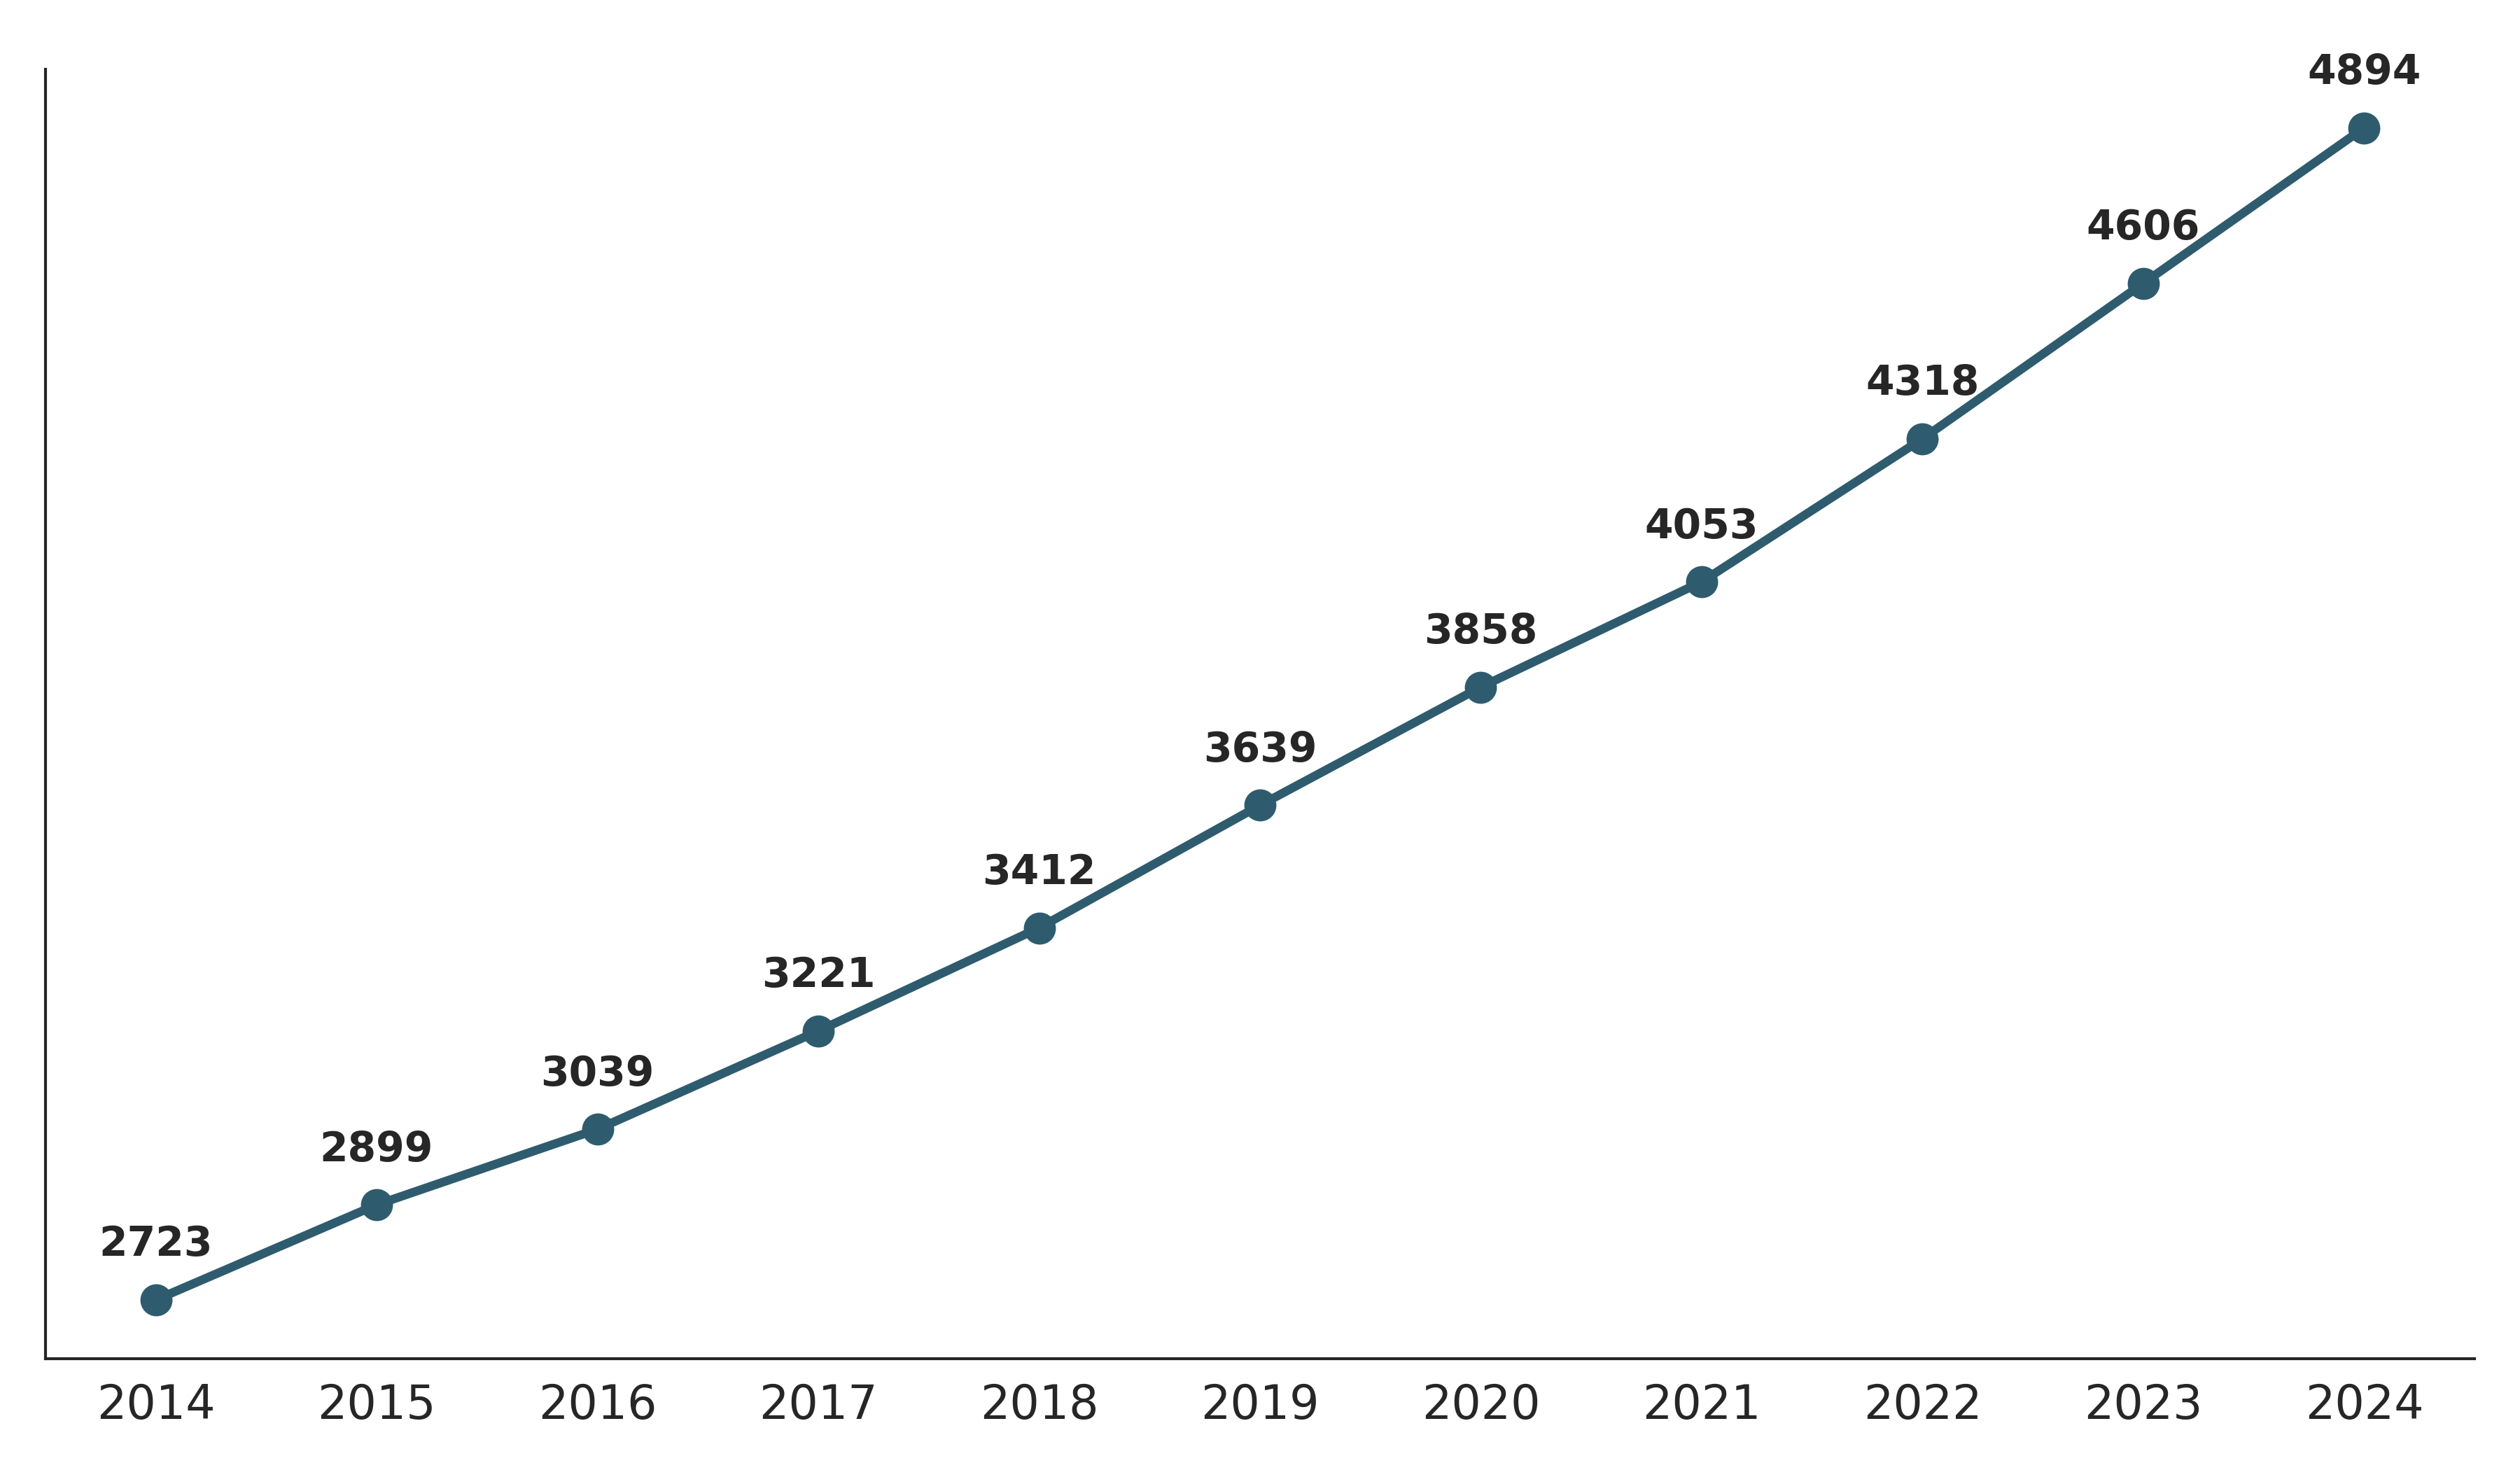
\includegraphics[width=\linewidth]{figures/n_assets_year.png}
    \caption{Number of assets in the dataset per year}
    \label{fig:n_assets}
\end{figure}

We first describe the global asset-class split and then summarize the composition of the universe. 

\subsection{Universe Composition}

\noindent Over the entire sample period, the absolute count of records is distributed primarily among individual stocks (3186 records) and Exchange-Traded Funds (ETFs) (1053 records), followed by Closed-End Funds (CEFs) (472 records) and Real Estate Investment Trusts (REITs) (183 records). For broader analytical purposes, we initially classify these into two macroeconomic groups: ``Stocks'' (individual equities) and ``Non-Stocks'' (ETFs, CEFs, and REITs).

Tables \ref{tab:global_count} and \ref{tab:global_mcap} present the temporal evolution of these two groups by count and market capitalization. The proportion of non-stocks grows steadily, from about one third of records in 2014 to nearly 45\% in 2024, largely driven by ETFs; their share of market value, however, remains near 16--19\% of the universe throughout.

\begin{table}[!htbp]
    % Overrides the rbfin.cls defaults to remove bold text and fix alignments
    \captionsetup{labelfont=normalfont, textfont=normalfont, justification=justified, singlelinecheck=off}
    \captionsetup[subtable]{labelfont=normalfont, textfont=normalfont, justification=centering, singlelinecheck=off}
    
    \centering
    
    % First subtable
    \begin{subtable}[t]{0.48\textwidth}
        \centering
        \begin{tabular}{lcc}
        \toprule
        Year & Stock (\%) & Non-Stock (\%) \\
        \midrule
        2014 & 65.00 & 35.00 \\
        2015 & 63.33 & 36.67 \\
        2016 & 61.76 & 38.24 \\
        2017 & 60.97 & 39.03 \\
        2018 & 59.88 & 40.12 \\
        2019 & 59.58 & 40.42 \\
        2020 & 58.76 & 41.24 \\
        2021 & 57.76 & 42.24 \\
        2022 & 56.81 & 43.19 \\
        2023 & 56.06 & 43.94 \\
        2024 & 55.23 & 44.77 \\
        \bottomrule
        \end{tabular}
        \caption{By total quantity}
        \label{tab:global_count}
    \end{subtable}%
    \hfill% Provides spacing between the two subtables
    % Second subtable
    \begin{subtable}[t]{0.48\textwidth}
        \centering
        \begin{tabular}{lcc}
        \toprule
        Year & Stock (\%) & Non-Stock (\%) \\
        \midrule
        2014 & 81.80 & 18.20 \\
        2015 & 82.66 & 17.34 \\
        2016 & 81.11 & 18.89 \\
        2017 & 81.24 & 18.76 \\
        2018 & 80.94 & 19.06 \\
        2019 & 81.04 & 18.96 \\
        2020 & 83.85 & 16.15 \\
        2021 & 83.58 & 16.42 \\
        2022 & 82.89 & 17.11 \\
        2023 & 82.76 & 17.24 \\
        2024 & 82.93 & 17.07 \\
        \bottomrule
        \end{tabular}
        \caption{By market capitalization}
        \label{tab:global_mcap}
    \end{subtable}
    
    \vspace{1em} % Adds a little breathing room before the main caption
    
    % Main caption underneath both tables
    \caption{Annual global distribution of asset classes. This table presents the relative percentage of non-stock entities (including Exchange-Traded Funds, Closed-End Funds, and Real Estate Investment Trusts) compared to individual stocks from 2014 to 2024. The progression highlights a continuous, decade-long structural shift toward non-stock investment vehicles within the dataset by quantity. Market-capitalization shares are reported for completeness; records with missing or unreported capitalization fields are excluded from the capitalization-based aggregates and therefore do not affect the proportions shown.}
    \label{tab:global_distribution}
\end{table}

\noindent Complete year-by-year breakdowns by vehicle type, sector, and industry are available from the authors on request. Within the non-stock segment, exchange-traded funds dominate and are growing, rising from 63.1\% of non-stock records in 2014 to 78.1\% in 2024 (and from 76.7\% to 87.1\% of non-stock market capitalization), while closed-end funds and REITs decline. Within the individual-stock segment, Financials and Industrials account for the largest number of firms, but market value is increasingly concentrated in Technology, whose capitalization share more than doubles over the decade, from 12.9\% to 29.7\%; Healthcare also expands markedly, from 13.0\% to 19.1\% of firms. These shifts matter for interpretation: the network core is populated by large, heavily traded firms, while the periphery is dominated by smaller, idiosyncratic names, and the composition of both evolves over the sample.

\section{Methodology}\label{sec:methodology}

\subsection{Correlation Matrix Estimation}

%In every section, the paragraph begins without indentation (Tradition in many scientific articles)
\noindent In order to build filtered correlation-based networks, we first develop a robust correlation matrix estimation procedure. For this study, we adopt a rolling-window approach spanning from 2014 to 2024, utilizing 5 years of past data to construct the correlation matrix for each target year.

To capture the time-varying nature of financial correlations while maintaining statistical robustness, we partition the 5-year lookback period into $K=5$ consecutive annual sub-windows, each comprising 252 trading days. Within each sub-window $k \in \{1, \dots, K\}$ (ordered chronologically), we estimate a well-conditioned covariance matrix $\boldsymbol{\Sigma}_k$ using the Ledoit-Wolf shrinkage estimator. This analytical approach minimizes the expected Frobenius norm between the estimated and true covariance matrices by optimally shrinking the sample covariance toward a constant-correlation target. This guarantees positive definiteness even in high-dimensional or noisy settings, without requiring ad-hoc parameter tuning.

To place greater emphasis on more recent market dynamics, we aggregate the sequence of shrunk covariance matrices $\{\boldsymbol{\Sigma}_1, \dots, \boldsymbol{\Sigma}_K\}$ using an exponentially weighted average:
\begin{equation}
    \bar{\boldsymbol{\Sigma}} = \sum_{k=1}^{K} w_k \boldsymbol{\Sigma}_k
\end{equation}
where the normalized weights $w_k$ are defined as:
\begin{align}
    w^0_k &= \exp\left(-\frac{K-k}{\tau}\right) \\
    w_k &= \frac{w^0_k}{\sum_{i=1}^K w^0_i}
\end{align}
For our 5-year rolling specification, we empirically set the decay parameter to $\tau = 2.5$. This parameter optimally balances the integration of recent topological innovations with historical structural stability. The resulting exponential weight distribution across the temporal windows can be seen in Figure \ref{fig:ew}.

Finally, the robust correlation matrix $\mathbf{C}$ utilized for the Triangulated Maximally Filtered Graph (TMFG) construction is derived directly from the exponentially weighted covariance matrix by standardizing its elements:
\begin{equation}
    C_{ij} = \frac{\bar{\Sigma}_{ij}}{\sqrt{\bar{\Sigma}_{ii} \bar{\Sigma}_{jj}}}
\end{equation}
To prevent any computational floating-point precision errors, we explicitly force the main diagonal elements of the resulting matrix to exactly 1.0. This rigorous pipeline guarantees that the final correlation matrix is strictly positive semi-definite, maintains a true unit diagonal, and achieves an optimal bias-variance trade-off prior to the graph filtering process.

\begin{figure}[!ht]
    \captionsetup{labelfont=normalfont, textfont=normalfont, justification=justified, singlelinecheck=off}
    \captionsetup[subtable]{labelfont=normalfont, textfont=normalfont, justification=centering, singlelinecheck=off}
    \centering
    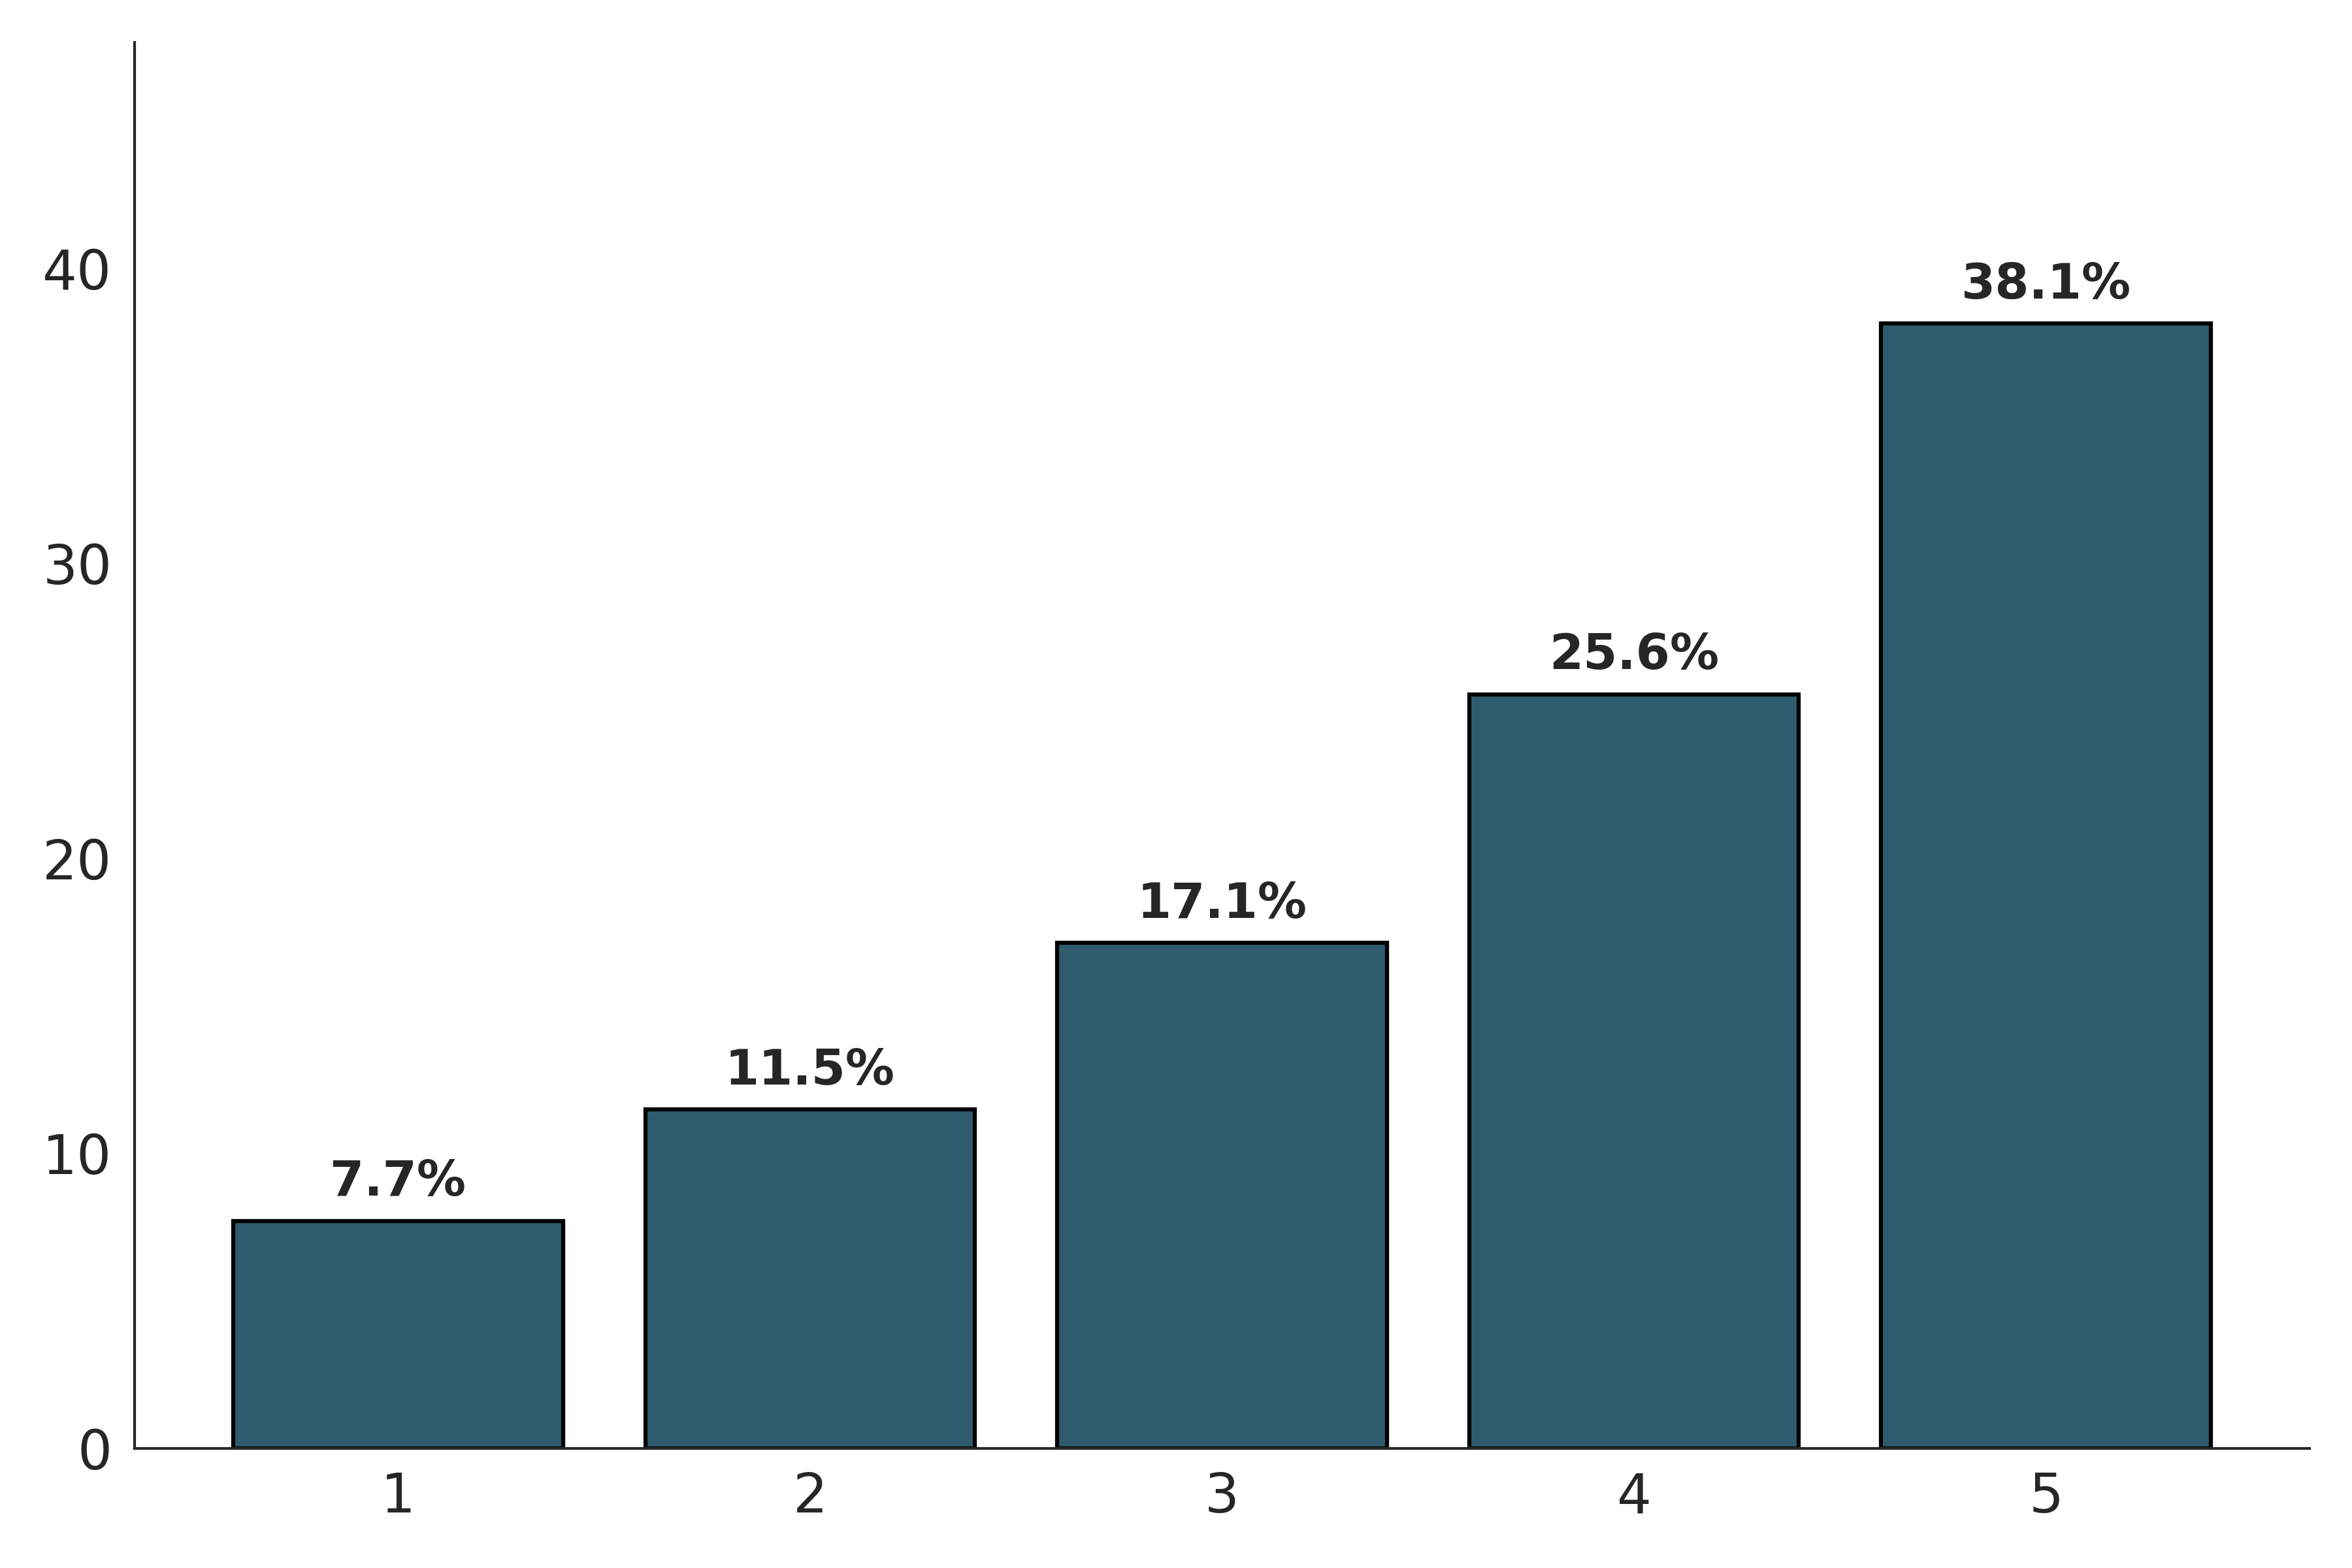
\includegraphics[width=\linewidth]{figures/exp_weights.png}
    \caption{Exponential weight distribution across temporal windows.}
    \label{fig:ew}
\end{figure}

\subsection{Triangular Maximally Filtered Graph}

\noindent Once the correlation matrices have been estimated using the robust shrinkage procedure, the subsequent step consists of extracting a meaningful network representation of the dependence structure among the assets. Because correlation matrices in financial markets are typically dense and contain a substantial amount of estimation noise, directly interpreting all pairwise relationships can obscure the most relevant economic connections. It is therefore necessary to apply a topological filtering procedure that preserves the most informative correlations while systematically reducing spurious links and dimensionality.

To achieve this, we employ the Triangulated Maximally Filtered Graph (TMFG). The TMFG is a deterministic, topology-based filtering technique designed to retain the most relevant dependencies within a correlation matrix while strictly enforcing a planar graph structure. 

The primary advantage of the TMFG lies in its optimal balance between information retention, structural complexity, and computational efficiency. Unlike the Minimum Spanning Tree (MST), which enforces a heavily restricted tree structure (yielding only $N-1$ edges) and often discards significant clustering information, the TMFG preserves a much larger, highly clustered subset of high-weight edges while maintaining planarity. Furthermore, while the Planar Maximally Filtered Graph (PMFG) also achieves a planar embedding, it requires computationally expensive planarity testing at every step, resulting in a computational complexity of $O(N^3)$. In contrast, the TMFG relies on a localized structural growth rule that inherently guarantees planarity, reducing the computational complexity to $O(N^2)$. This efficiency is crucial for our methodology, as it allows the algorithm to scale seamlessly to large cross-sections of assets evaluated over numerous rolling estimation windows.

Based on our implementation, the construction of the TMFG proceeds through a deterministic, greedy algorithmic expansion. Let $\mathbf{C}$ be the input matrix constructed from the absolute values of the robust correlation matrix. The network topology is generated through the following steps:

\begin{enumerate}
    \item \textbf{Initialization (The Seed Clique):} We first compute the node strength $s_i$ for each asset $i$, defined as the sum of its absolute correlations with all other assets: $s_i = \sum_{j} C_{ij}$. The four assets exhibiting the highest overall strengths are selected to form the initial network seed. These four nodes are fully connected to form a 4-clique (a tetrahedron), which intrinsically defines four initial triangular faces.
    
    \item \textbf{Gain Evaluation:} At each subsequent step, the algorithm evaluates all nodes that have not yet been integrated into the network. For every candidate node $v$ and every active triangular face $f = \{i, j, k\}$ in the graph, we compute a gain function representing the sum of the absolute correlations between the candidate node and the three vertices of the face:
    \begin{equation}
        g(v, f) = C_{vi} + C_{vj} + C_{vk}
    \end{equation}
    
    \item \textbf{Vertex Insertion (Winner-Take-All):} The algorithm identifies the global maximum gain across all available node--face pairs. The winning node $v^*$ is inserted into the network by establishing edges with the three vertices $\{i, j, k\}$ of its optimal face $f^*$.
    
    \item \textbf{Face Updating:} The insertion of $v^*$ geometrically transforms the selected face $f^*$ into a new tetrahedral structure. Consequently, the original face $f^*$ is removed from the list of active faces, and three new triangular faces—$\{v^*, i, j\}$, $\{v^*, i, k\}$, and $\{v^*, j, k\}$—are generated and made available for future attachments. The gains for the remaining unconnected nodes are then efficiently updated to account for these newly formed faces.
    
    \item \textbf{Termination:} Steps 2 through 4 are repeated iteratively until all $N$ assets have been successfully incorporated into the graph.
\end{enumerate}

By mathematically constraining the growth process to tetrahedral expansions, the resulting graph is guaranteed to be planar and composed of a nested hierarchy of 4-cliques. This planarity constraint ensures a strict topological sparsity, yielding exactly $3N - 6$ edges. This specific density effectively filters out noisy, low-significance correlations and prevents structural overfitting, while the greedy gain-maximization step guarantees that the strongest local dependencies are preferentially retained.

In our framework, this TMFG-filtered network serves as the structural backbone for computing centrality measures and segregating central stocks from peripheral ones. By systematically capturing the core hierarchical structure of return interdependencies and mitigating estimation noise, the TMFG proves uniquely suited for analyzing market leadership dynamics and constructing topology-driven portfolios.

\subsection{Network Centrality Metric}

\noindent Having filtered the network, we now quantify the structural importance of each node. Network centrality measures summarize a node's position and let us distinguish stocks that occupy interconnected, influential positions from those on the periphery; this classification underpins our topology-based portfolio construction and the lead--lag analysis.

For the construction of our network centrality metric, we depart from the approach proposed by \citet{pozzi2013spread}. In their framework, the authors compute a broad set of centrality measures (degree ($D$), betweenness centrality ($BC$), eccentricity ($E$), closeness ($C$), and eigenvector centrality ($EC$)) for both weighted ($w$) and unweighted ($u$) versions of the network.

In the weighted case, different transformations of the correlation matrix are employed depending on the metric. For weighted degree and weighted eigenvector centrality, the edge weight is defined as $1 + \bar{R}_{ij}^w$, where $\bar{R}_{ij}^w$ denotes the filtered correlation between nodes $i$ and $j$. For the remaining metrics (betweenness, eccentricity, and closeness) the weight is instead defined through a distance transformation given by the Euclidean metric
\[
d_{ij} = \sqrt{2\left(1 - \bar{R}_{ij}^w\right)}.
\]
This transformation maps correlations into distances, ensuring that strongly correlated nodes are closer in network space.

After computing all centrality measures, \citealt{pozzi2013spread} analyze the similarity of node rankings induced by each metric. By clustering these rankings, they identify two distinct groups. The first cluster comprises degree and betweenness centrality (both weighted and unweighted), while the second cluster includes eccentricity, closeness, and eigenvector centrality (again in both weighted and unweighted forms). Based on this empirical partition, they define two composite indicators:

\begin{align}
    X &= \dfrac{D^u + D^w + BC^u + BC^w - 4}{4(N-1)}, \\
    Y &= \dfrac{E^u + E^w + C^u + C^w + EC^u + EC^w - 6}{6(N-1)},
\end{align}

\noindent where $N$ denotes the number of nodes in the network, and the normalization ensures that both $X$ and $Y$ lie in the unit interval. The subtraction terms account for the minimum attainable values of the rankings.

Depending on the signs of $X$ and $Y$, nodes range from strongly embedded in the core (small $X$, small $Y$) to deeply peripheral (large $X$, large $Y$), with hub-like and satellite configurations in between.

From these definitions, the sum $X+Y$ serves as an overall measure of centrality: it is small for central vertices and large for peripheral ones. In contrast, the difference $X-Y$ captures the nature of a node’s connections. A large value of $X-Y$ indicates that the vertex has few but important connections (i.e., links to central nodes), whereas a small value reflects many but relatively unimportant connections.

While this approach provides a rich characterization of node roles, its reliance on rank-based transformations introduces significant limitations for quantitative portfolio allocation. Rank-based metrics inherently discard the magnitude of structural differences between nodes. In financial networks, which often exhibit highly skewed degree distributions, the topological distance between the first and second most central nodes may be vastly different than the distance between the fiftieth and fifty-first. To overcome this limitation and obtain a more robust proxy for structural importance, we propose a continuous, data-driven Network Centrality Metric. Our methodology focuses on a transparent aggregation of a set of complementary centrality measures that capture local connectivity, global accessibility, and recursive influence. We begin by transforming the filtered correlation weights into a proper metric space. For each edge $(i,j)$ with correlation $C_{ij}$, we define the distance as
\begin{equation}
    d_{ij} = \sqrt{2(1 - C_{ij})}
\end{equation}

\noindent Unlike simple reciprocal transformations, this Euclidean mapping satisfies the triangle inequality, is bounded between $0$ (perfect positive correlation) and $\sqrt{2}$ (zero correlation), and ensures numerical stability for shortest-path calculations. Because the TMFG is constructed on absolute correlations, both the similarity weights used by degree and eigenvector centrality and the distances used by closeness centrality are derived from the magnitude of the correlation, $|C_{ij}|$. We then compute three standard centrality measures for each node $i$:

\begin{enumerate}
    \item \textbf{Weighted degree centrality.}  
    The sum of the absolute correlations of its adjacent edges, capturing local connectedness and direct market linkages:
    \begin{equation}
    \text{Degree}_i = \sum_{j} |C_{ij}|.
    \end{equation}
    This measure reflects how strongly a stock is directly linked to others.

    \item \textbf{Closeness centrality.}  
    The inverse of the average shortest-path distance to all other nodes, indicating how quickly a stock can transmit shocks across the global network structure:
    \begin{equation}
    \text{Closeness}_i = \left( \frac{1}{N-1} \sum_{j \neq i} d_{ij}^{\text{shortest}} \right)^{-1} = \frac{N-1}{\sum_{j \neq i} d_{ij}^{\text{shortest}}},
    \end{equation}
    where $d_{ij}^{\text{shortest}}$ is the shortest-path distance induced by the edge distances $d_{ij}=\sqrt{2\,(1-|C_{ij}|)}$.

    \item \textbf{Eigenvector centrality.}  
    A measure of recursive influence that assigns higher values to nodes connected to other highly central nodes, capturing systemic importance:
    \begin{equation}
    \mathbf{A}\mathbf{x} = \lambda \mathbf{x},
    \end{equation}
    where $\mathbf{A}$ is the weighted adjacency matrix with entries $A_{ij}=|C_{ij}|$ for connected nodes and zero otherwise, consistent with the use of absolute correlations in the TMFG construction.
\end{enumerate}

Because these metrics operate on fundamentally different scales, we standardize each cross-sectionally using Z-scores

\begin{equation}
    Z_{M,i} = \frac{M_i - \mu_M}{\sigma_M}
\end{equation}

\noindent This standardization prevents extreme network outliers from dominating the distribution and ensures temporal comparability across our rolling estimation windows. Finally, we construct the Network Centrality Metric as a convex combination of the standardized measures 
\begin{equation}
    \text{Hybrid}_i = -(\omega_D Z_{D,i} + \omega_C Z_{C,i} + \omega_{EC} Z_{EC,i})
\end{equation}

\noindent where $\omega_D + \omega_C + \omega_{EC} = 1$. The multiplication by $-1$ occurs to force the same interpretation as Pozzi's metric, where small values represent central nodes and large values represent peripheral nodes. Rather than imposing an ad-hoc weighting scheme, we determine the vector of weights $\boldsymbol{\omega}$ dynamically for each estimation window using Principal Component Analysis (PCA). We extract the first principal component (PC1) from the cross-sectional covariance matrix of the three standardized centrality measures. Because principal-component loadings are defined only up to a sign, we take their absolute values and normalize them to sum to unity; this yields a non-negative convex weighting that is invariant to the arbitrary orientation of the eigenvector. Because the weights adapt within each window, the contribution of each centrality dimension is proportional to the topological variance it explains at that time, providing an objective consensus of a node's systemic importance without arbitrary hyperparameters. Stocks with high hybrid scores are classified as peripheral and those with low scores as central, forming the basis for the lead--lag analysis and the topology-based portfolios below.

Relative to the rank-based composite of \citet{pozzi2013spread}, our construction is simpler and scale-explicit, and it avoids the redundancy of combining weighted and unweighted variants of the same metrics \citep{Bonacich1972}. The contribution is not the aggregation of centrality measures per se---composites of this kind are well established---but the data-driven PCA weighting and the preservation of the magnitude of structural differences. Because it relies on normalized values and linear aggregation, it is also stable and scalable in large networks.

\subsection{Quantitative Portfolio Formulation}

Having established that central market hubs lead peripheral assets due to friction-induced information delays, we now turn to the economic significance of this phenomenon. To formalize an institutional investment framework that exploits this structural asymmetry, we implement a quantitative portfolio optimization utilizing the Treynor-Black (1973) model. The framework is designed to isolate the network-driven alpha generated by the topological extremes.

\vskip 2em
\noindent\textbf{Market Benchmark Formulation}
To accurately evaluate the active tilts generated by our network signals, we require a representative baseline. Unlike naïve equal-weighted ($1/N$) approaches, we define our market benchmark as a value-weighted portfolio comprising all assets across all network deciles, from the central core ($D_1$) to the absolute periphery ($D_{10}$). The capitalization-weighted benchmark weights, $\omega_{m, i, t}$, and the resulting market return, $R_{m, t}$, are formulated as:
\begin{equation}
    \omega_{m, i, t} = \frac{\text{MCap}_{i, t}}{\sum_{j \in \mathcal{U}_t} \text{MCap}_{j, t}}, \quad \forall i \in \mathcal{U}_t = \bigcup_{k=1}^{10} D_{k, t}
\end{equation}
\begin{equation}
    R_{m, t} = \sum_{i \in \mathcal{U}_t} \omega_{m, i, t} R_{i, t}
\end{equation}
Anchoring on this full capitalization universe ensures that the benchmark reflects the true, unconstrained opportunity set of the market. Consequently, the active network tilts are rigorously measured against the broadest possible market baseline.

\vskip 2em

\noindent\textbf{Single-Index Model (SIM) Estimation and Network Alpha Selection}
To extract the specific alpha components for our active portfolio, we estimate the Sharpe (1963) Single-Index Model (SIM). The SIM is calibrated strictly over the rolling 1-year window $t-1$ preceding each investment period:
\begin{equation}
    R_{i, \tau} - R_{f, \tau} = \alpha_i + \beta_i (R_{m, \tau} - R_{f, \tau}) + e_{i, \tau}, \quad \tau \in \mathcal{T}_{t-1}
\end{equation}
where $\alpha_i$ represents the annualized Jensen's alpha, $\beta_i = \frac{\text{Cov}(R_i, R_m)}{\text{Var}(R_m)}$ denotes the systematic market exposure, and $\sigma_{ei}^2 = \text{Var}(e_i)$ is the idiosyncratic residual variance of the asset.

Our preceding empirical results demonstrate that the central portfolio (Decile 1) acts as a high-beta systematic conduit with significant negative alpha, whereas the peripheral portfolio (Decile 10) attenuates this footprint and generates significant positive alpha. Therefore, we apply a strict topological alpha screening process:
\begin{itemize}
    \item \textbf{Long Candidates ($\mathcal{A}^{+}$):} Peripheral stocks ($i \in D_{10}$) exhibiting positive estimated alpha ($\hat{\alpha}_i > 0$).
    \item \textbf{Short/Underweight Candidates ($\mathcal{A}^{-}$):} Central stocks ($j \in D_1$) exhibiting negative estimated alpha ($\hat{\alpha}_j < 0$).
\end{itemize}
Assets presenting inconsistent signs ($\hat{\alpha}_i \le 0$ in $D_{10}$ or $\hat{\alpha}_j \ge 0$ in $D_1$) are systematically excluded from active bets to maintain signal purity. Because each decile contains several hundred assets, we further concentrate the bets by retaining, in each extreme decile, only the 25 candidates with the largest absolute estimated alpha.

\vskip 2em

\noindent\textbf{Treynor-Black Active Portfolio Construction}
The active portfolio $\mathcal{A}$ allocates capital among the selected candidates based on the \citealp{treynorblack73} idiosyncratic weighting rule, which scales positions by the appraisal ratio:
\begin{equation}
    \omega_{A, i}^0 = \frac{\hat{\alpha}_i}{\hat{\sigma}_{ei}^2}
\end{equation}
We evaluate two institutional implementations of this strategy:
\begin{enumerate}
    \item \textbf{Treynor-Black Unconstrained:} This approach permits simultaneous long positions in the periphery ($D_{10}$) and short positions in the core ($D_1$), with weights normalized as:
    \begin{equation}
        \omega_{A, i} = \frac{\omega_{A, i}^0}{\sum_{k \in \mathcal{A}} |\omega_{A, k}^0|}
    \end{equation}
    \item \textbf{Treynor-Black Long-Only:} This implementation prohibits short selling, restricting active positions strictly to peripheral assets demonstrating positive alpha:
    \begin{equation}
        \omega_{A, i} = \frac{\omega_{A, i}^0}{\sum_{k \in \mathcal{A}^{+}} \omega_{A, k}^0}, \quad \forall i \in \mathcal{A}^{+}
    \end{equation}
\end{enumerate}

The implied aggregate active alpha, beta and residual variance are recorded as diagnostics:
\begin{equation}
    \alpha_A = \sum_{i \in \mathcal{A}} \omega_{A, i} \hat{\alpha}_i, \quad \beta_A = \sum_{i \in \mathcal{A}} \omega_{A, i} \hat{\beta}_i, \quad \sigma_{eA}^2 = \sum_{i \in \mathcal{A}} \omega_{A, i}^2 \hat{\sigma}_{ei}^2
\end{equation}
To enforce a realistic institutional tracking-error mandate we fix the active budget at $w_A = 0.20$ and apply the active weights as a tilt on the capitalization-weighted benchmark:
\begin{equation}
    w_{i, t} =
    \begin{cases}
        \omega_{m, i, t} + w_A \, \omega_{A, i, t}, & i \in \mathcal{A}^{+}, \\[2pt]
        \omega_{m, i, t} - w_A \, |\omega_{A, i, t}|, & i \in \mathcal{A}^{-}, \\[2pt]
        \omega_{m, i, t}, & \text{otherwise},
    \end{cases}
\end{equation}
followed by renormalization so that $\sum_i w_{i, t} = 1$; the long-only variant clips negative weights at zero before renormalizing. This bounds the active share at approximately 20\% while preserving broad market diversification.

\vskip 2em

\noindent\textbf{Walk-Forward Protocol and Transaction Costs}
To ensure rigorous performance evaluation, we impose a strict walk-forward, out-of-sample testing protocol devoid of lookahead bias. Rebalancing is conducted annually. For any trading year $t \in [2015, 2024]$, all network centralities, decile classifications, SIM parameters ($\hat{\alpha}_i, \hat{\beta}_i, \hat{\sigma}_{ei}^2$), and target weights are determined using exclusively realized returns up to the conclusion of year $t-1$. The year 2014 serves exclusively as a lookback calibration window (warm-up year), resulting in a pure out-of-sample testing horizon spanning 10 full years (2,516 trading days).

To accurately reflect institutional implementation, performance is evaluated net of trading frictions. The total portfolio turnover at each annual rebalancing date $t$ is calculated as:
\begin{equation}
    \text{Turnover}_t = \sum_{i} |w_{i, t} - w_{i, t^-}|
\end{equation}
where $w_{i, t^-}$ denotes the drifted portfolio weights immediately prior to rebalancing. We apply a flat institutional transaction cost drag of 10 basis points ($c = 0.0010$) to all turnover, yielding the net daily return:
\begin{equation}
    R_{\text{net}, t} = R_{\text{gross}, t} - c \sum_i |w_{i, t} - w_{i, t^-}|
\end{equation}

We then formalize convex combinations of the network strategy with the risk-free asset ($R_f$) to construct the Capital Allocation Line (CAL):
\begin{equation}
    R_{c, t} = w_{\text{RF}} R_{f, t} + (1 - w_{\text{RF}}) R_{p, t}, \quad w_{\text{RF}} \in [0,1]
\end{equation}

\section{Results}\label{sec:results}

\subsection{Network Portfolio Composition}

\noindent For the selection of portfolio constituents, we divide the assets into deciles based on the Hybrid Centrality Metric (HCM) and the Pozzi metric, where the 1st decile represents the central assets, and the 10th decile comprises the peripheral assets. The union of these two groups forms our network-based portfolio universe. This decile-based rule ensures a clear structural separation between highly central and strongly peripheral assets while maintaining a sufficiently diversified set of securities within each group. Furthermore, it allows us to analyze behavioral patterns across the intermediate deciles.

Figure \ref{fig:hetmap_deciles} presents a heatmap illustrating the intersection of assets across deciles 1 through 10 for both the HCM and Pozzi metrics. We observe very little overlap in the first decile (central assets) between the two metrics, with only 4\% of the assets being shared. Specifically, the first HCM decile is primarily composed of assets that fall into the second (39\%) and sixth (46\%) Pozzi deciles, whereas the first Pozzi decile consists of assets spread between the second and fifth HCM deciles. In contrast, the tenth decile (peripheral assets) exhibits a much higher level of agreement, with 57\% of the assets overlapping. The vast majority of the remaining assets in this tail end fall into the ninth decile of the opposing metric. This demonstrates that while the two methodologies strongly agree on the identification of peripheral assets, there is substantial divergence in how they classify central assets.

\begin{figure}[!htbp]
    \captionsetup{labelfont=normalfont, textfont=normalfont, justification=justified, singlelinecheck=off}
    \captionsetup[subtable]{labelfont=normalfont, textfont=normalfont, justification=centering, singlelinecheck=off}
    \centering
    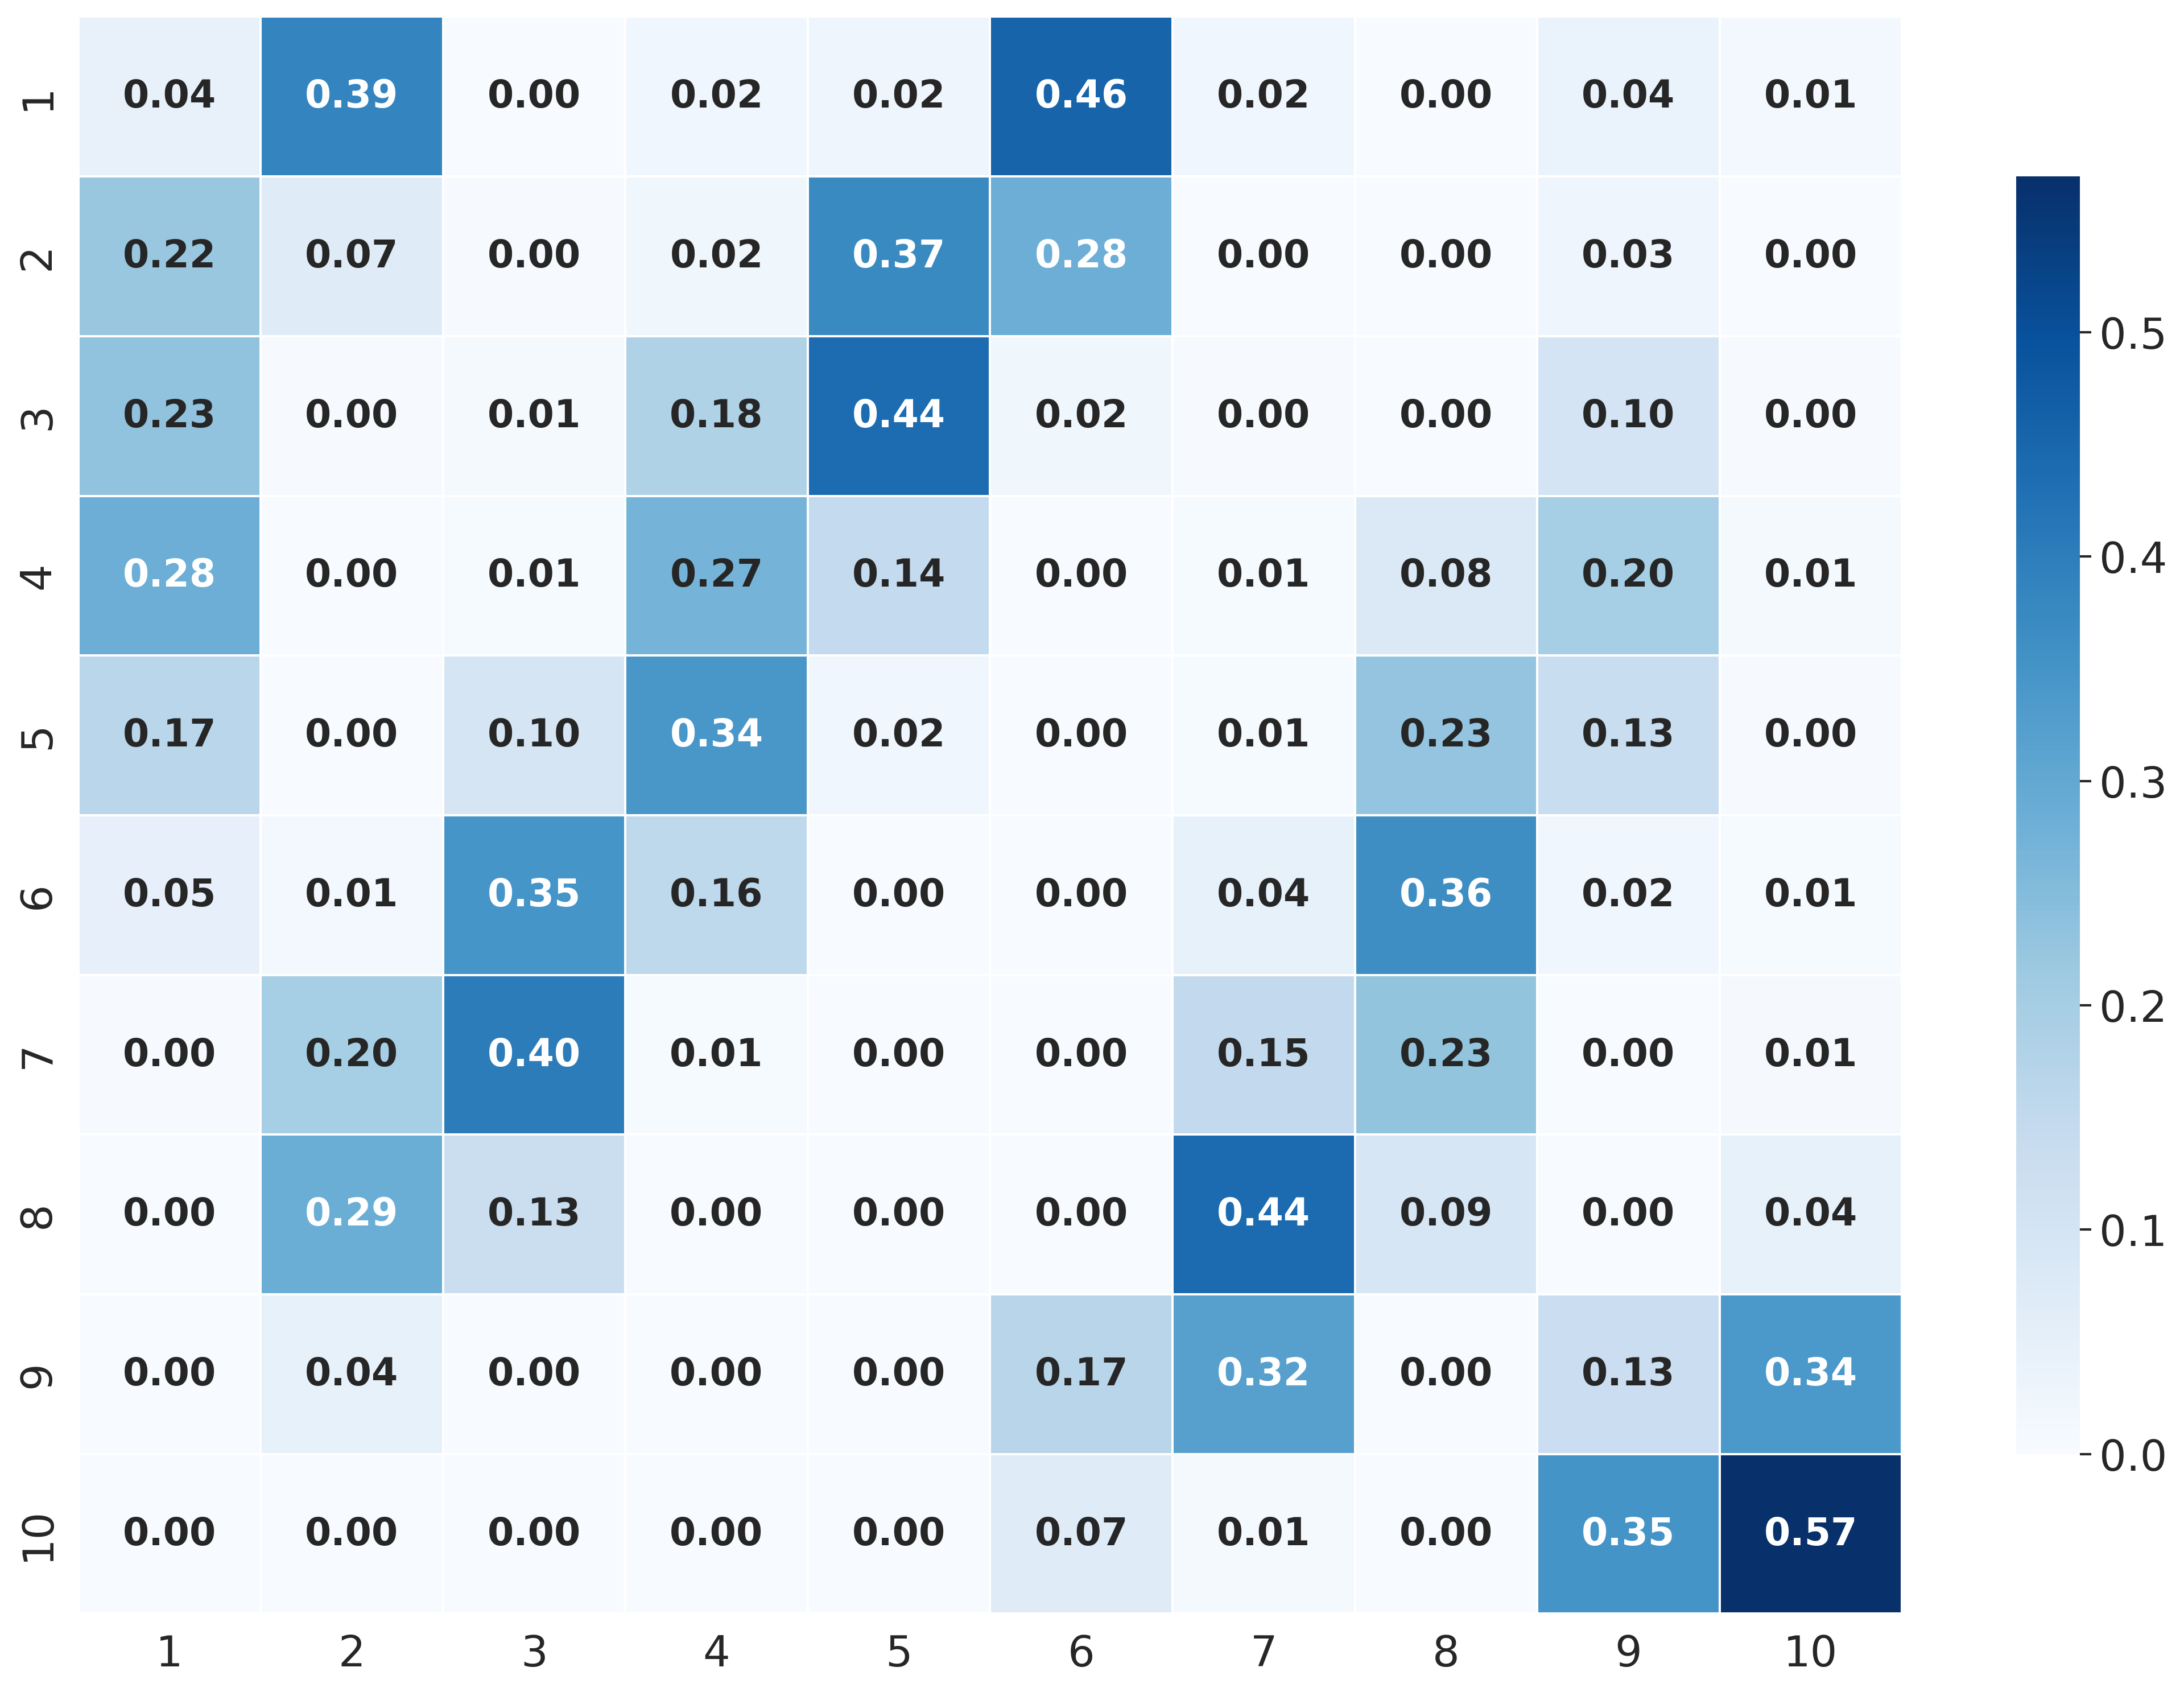
\includegraphics[width=\linewidth]{figures/heatmap_dispersao_hcm_pozzi.png}
    \caption{Heatmap displaying the overlap of portfolio deciles, mapping the Pozzi metric along the x-axis against the HCM metric along the y-axis.}
    \label{fig:hetmap_deciles}
\end{figure}

\begin{figure}[!htbp]
    \captionsetup{labelfont=normalfont, textfont=normalfont, justification=justified, singlelinecheck=off}
    \captionsetup[subfigure]{labelfont=normalfont, textfont=normalfont, justification=centering, singlelinecheck=off}
    \centering
    \begin{subfigure}{\linewidth}
        \centering
        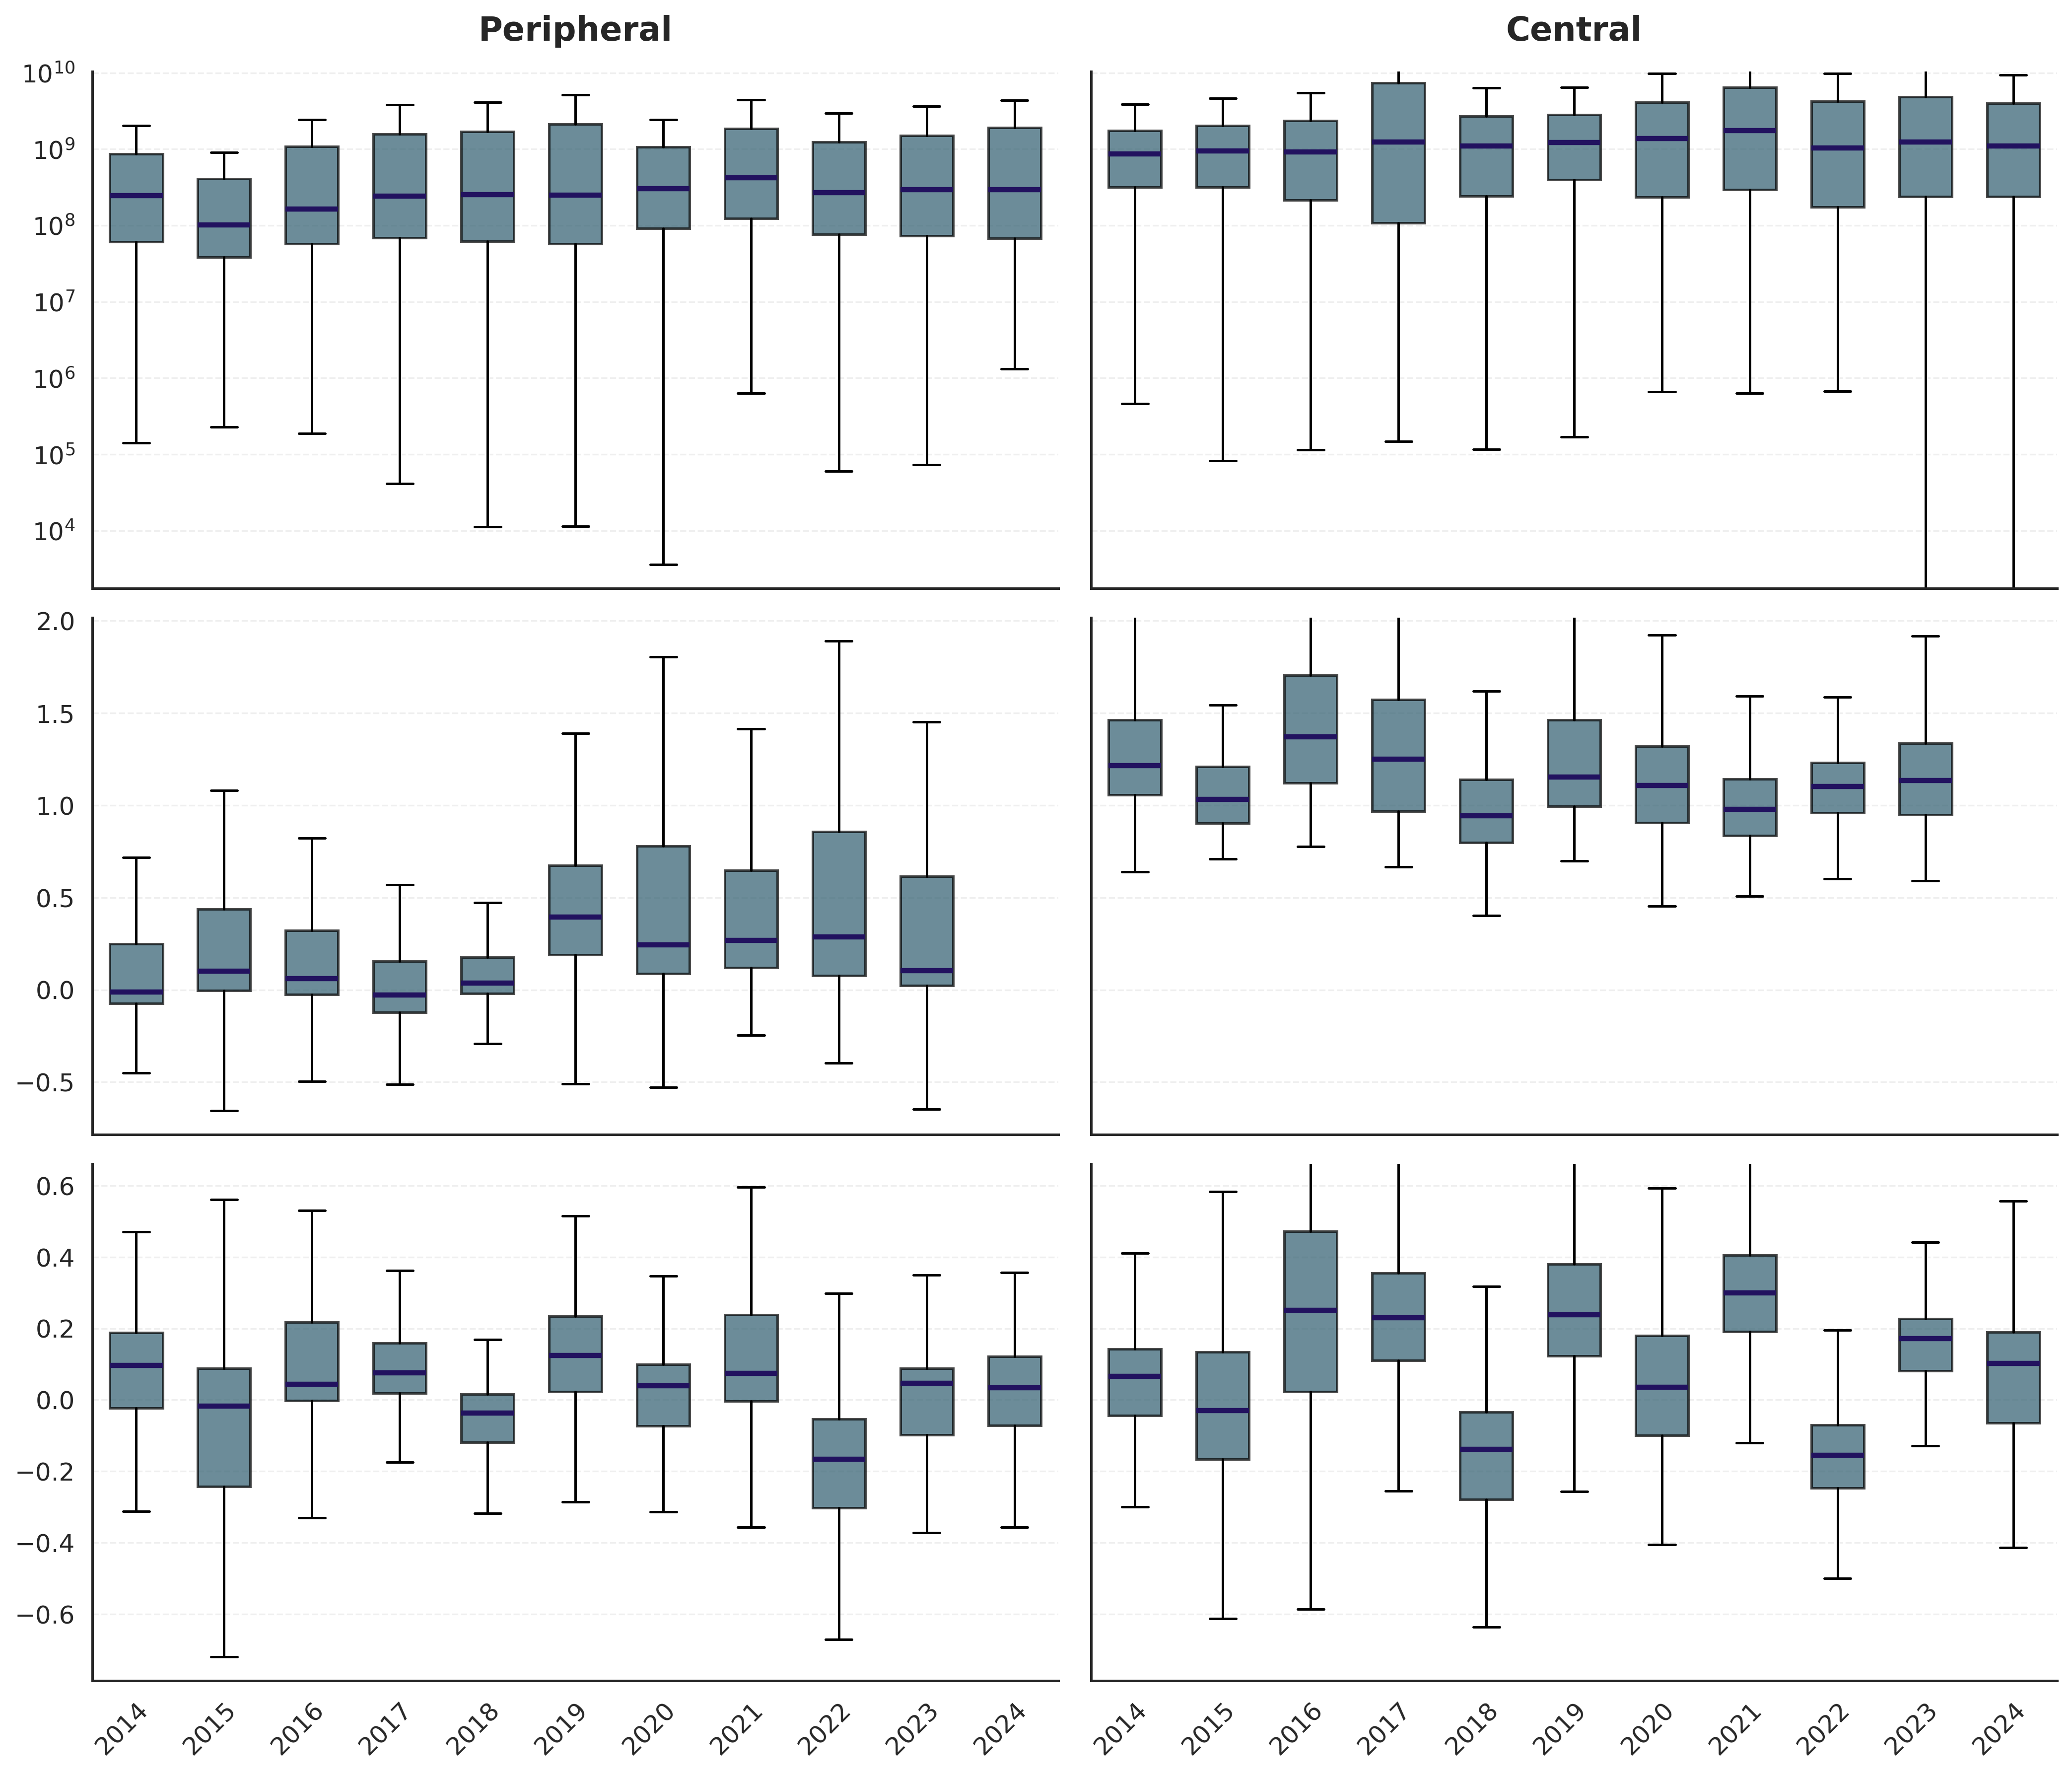
\includegraphics[width=0.70\linewidth]{figures/combined_metrics_evolution_hcm.png}
        \caption{Hybrid Centrality Metric}
        \label{fig:hcm_characteristics}
    \end{subfigure}

    \vspace{0.5em} 

    \begin{subfigure}{\linewidth}
        \centering
        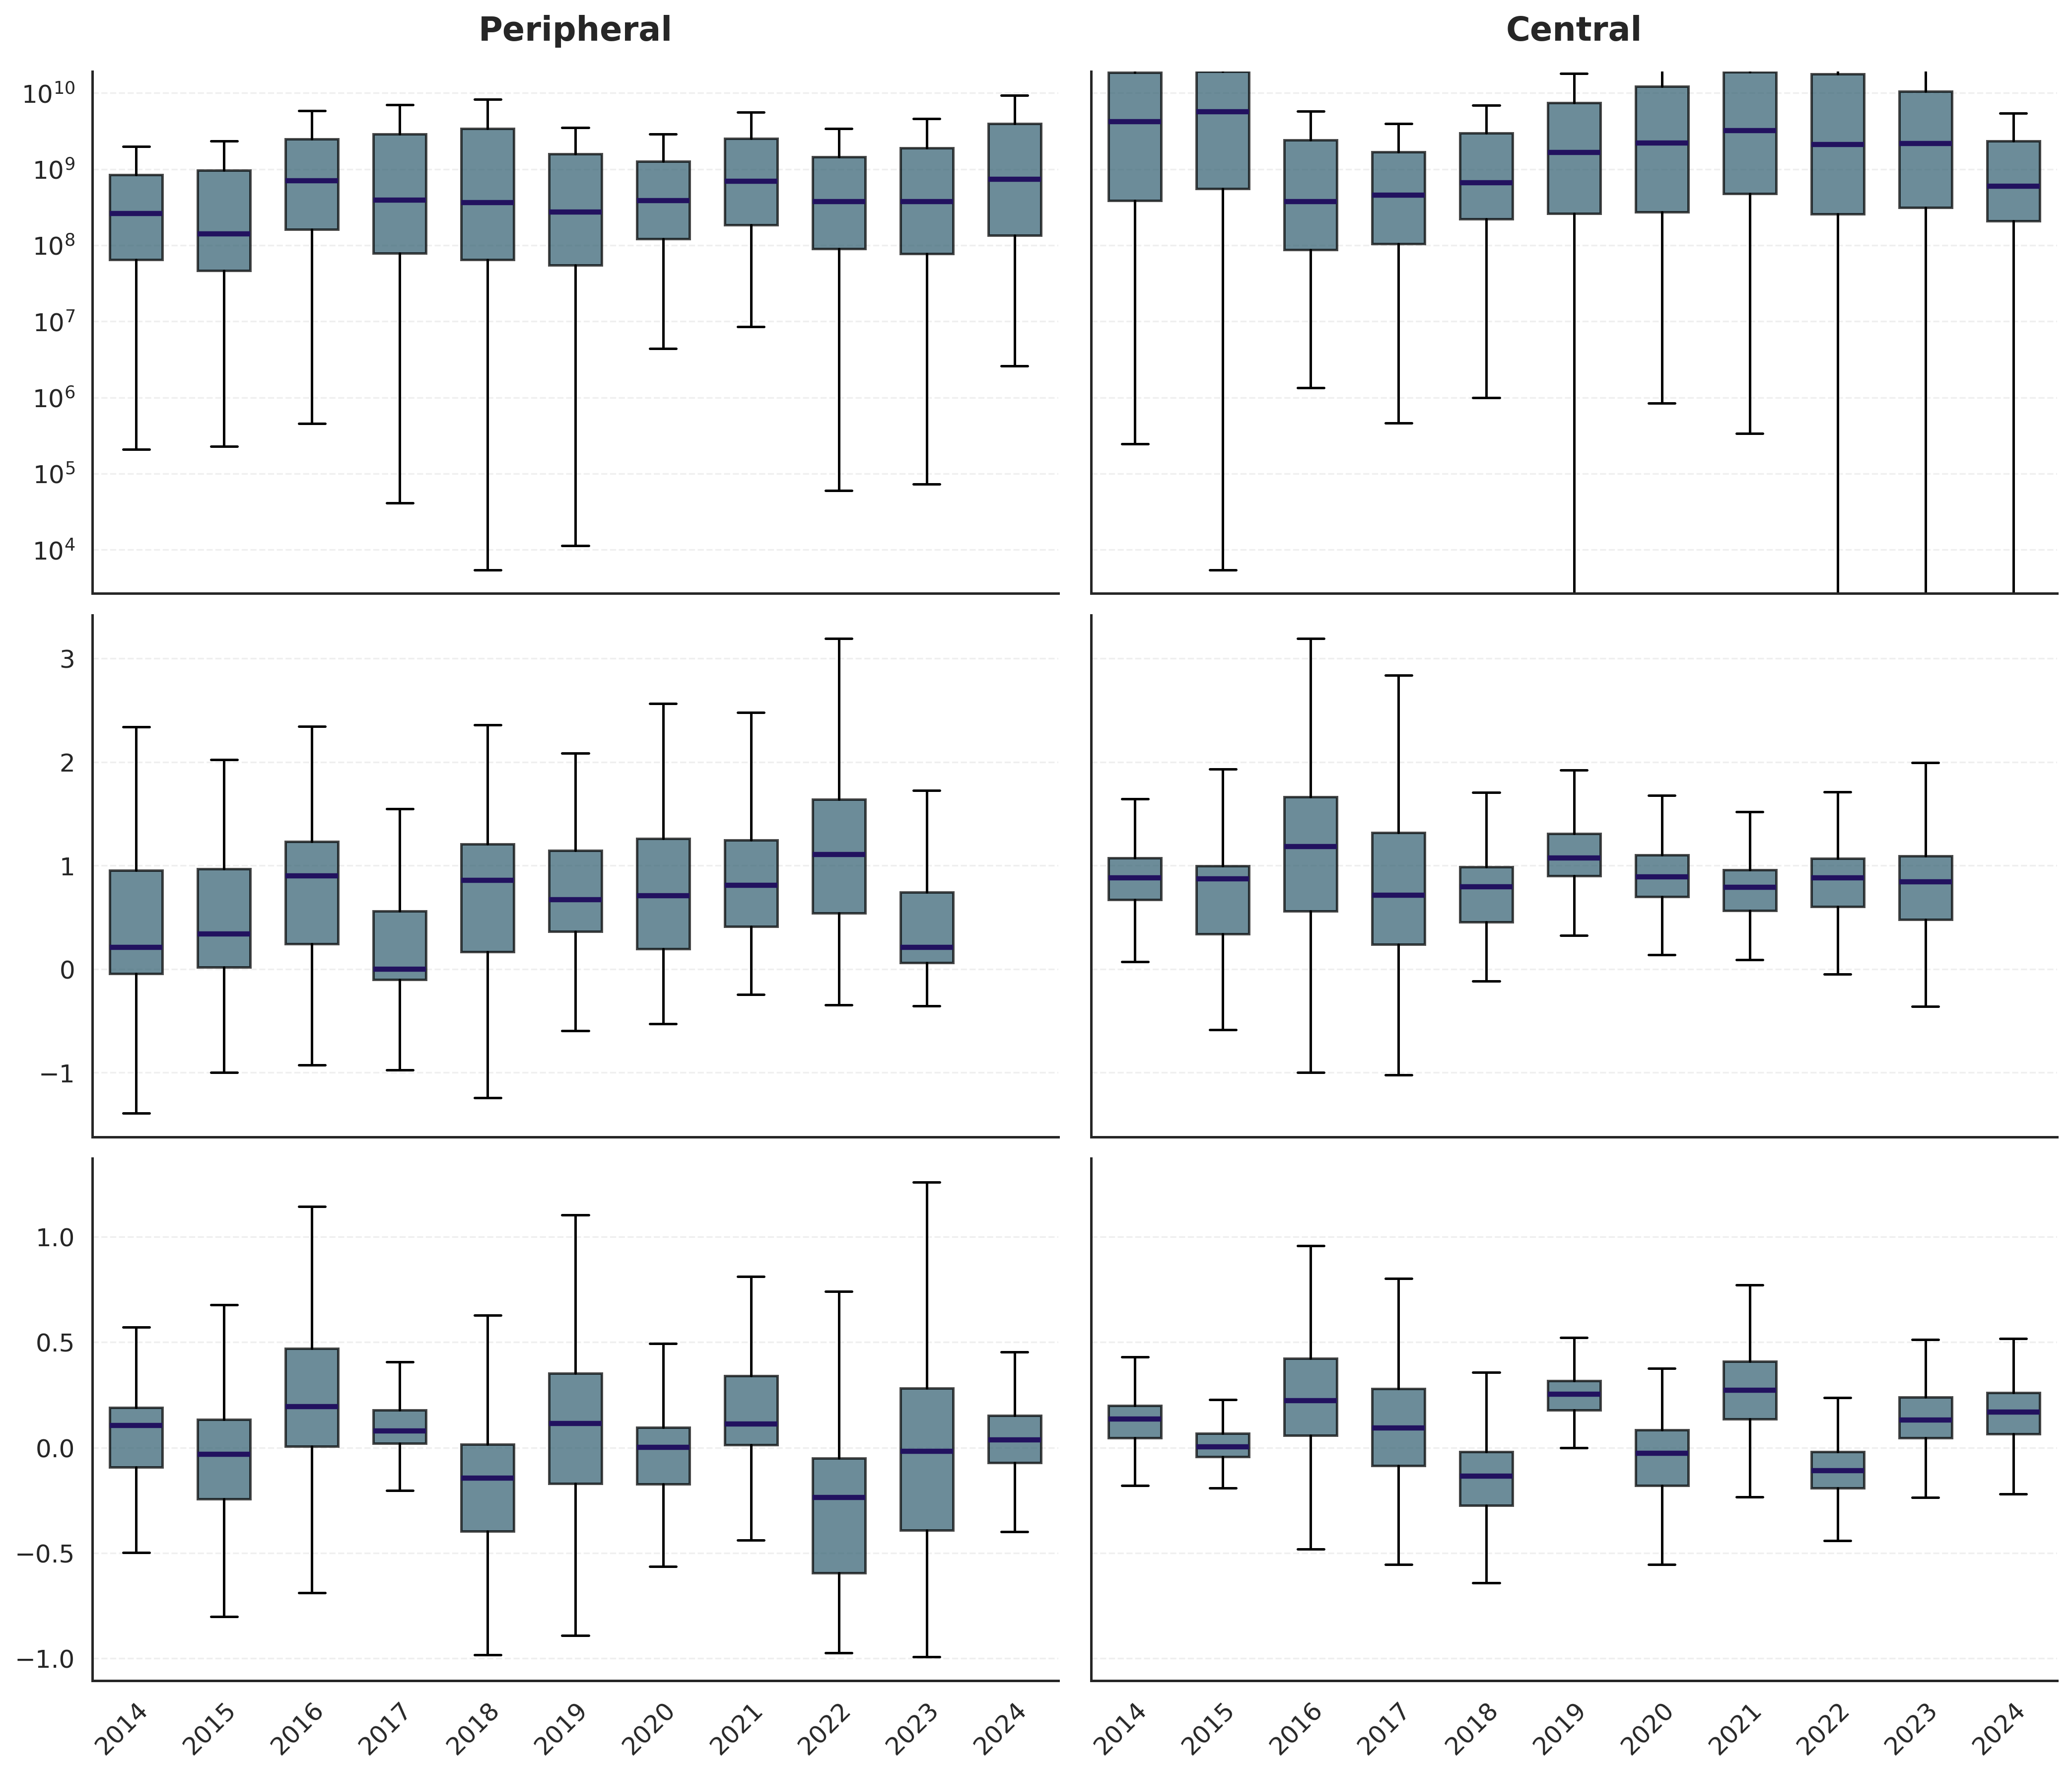
\includegraphics[width=0.70\linewidth]{figures/combined_metrics_evolution_pozzi.png}
        \caption{Pozzi Metric}
        \label{fig:pozzi_characteristics}
    \end{subfigure}
    \caption{Cross-sectional distributions of firm-level characteristics (Log Market Capitalization, Beta, and 12-month Momentum) for Central and Peripheral portfolios spanning 2014--2024 across both metrics. }
    \label{fig:combined_characteristics}
\end{figure}

Figures \ref{fig:hcm_characteristics} and \ref{fig:pozzi_characteristics} present the cross-sectional distributions of firm-level characteristics, Log Market Capitalization, Beta, and 12-month Momentum, for the Central and Peripheral portfolios from 2014 to 2024, comparing the HCM and Pozzi metrics, respectively. The comparative analysis of these boxplots reveals critical structural differences in how each methodology partitions the network.

\vskip 2em
\noindent\textbf{Market Capitalization }Both metrics exhibit a strong consensus regarding the size profile of the network's topology. Across both the HCM and Pozzi frameworks, the Central portfolio demonstrates a distinct size premium. Central assets consistently feature higher median market capitalizations (clustering around the $10^9$ range) and tighter interquartile distributions, confirming that the core of the correlation network is anchored by massive, heavily traded equities. Conversely, the Peripheral portfolios for both metrics capture the market's "long tail." While their medians are lower, the defining feature of the periphery is its massive downward dispersion, with whiskers frequently extending into the micro-cap territory at the bottom of the log-scale axis. Thus, structurally, both metrics agree that market centrality is intrinsically linked to firm size.

\vskip 2em
\noindent\textbf{The Beta Divergence }The most profound divergence between the two methodologies is observed in the distribution of Beta (the middle panels). The HCM metric (Figure \ref{fig:hcm_characteristics}) achieves a highly stable and clean partitioning of systematic risk. The HCM Central portfolio is entirely populated by high-beta assets (medians consistently between 1.0 and 1.5), representing the market's systematic drivers. Remarkably, the HCM Peripheral portfolio consistently isolates assets with near-zero systematic risk; from 2014 to 2018, its median Beta is almost exactly 0.0, rising only slightly in later years but remaining highly compressed. This indicates that HCM effectively separates systematically driven assets from purely idiosyncratic ones.

In stark contrast, the Pozzi metric (Figure \ref{fig:pozzi_characteristics}) fails to maintain a stable risk profile, particularly in the periphery. While the Pozzi Central portfolio also captures beta near 1.0, the Pozzi Peripheral portfolio is highly unstable. Rather than isolating zero-beta assets, the Pozzi periphery undergoes wild regime shifts. For instance, while its median beta is low in 2014 and 2018, it spikes in 2016, 2020, and most notably in 2023, where the median peripheral Beta actually \textit{exceeds} 1.0. This indicates that under the Pozzi metric, high-beta stocks can suddenly be relegated to the periphery during specific market shocks, reflecting transient correlation breakdowns rather than stable structural isolation.

\vskip 2em
\noindent\textbf{12-Month Momentum }The bottom panels detailing 12-month Momentum further reinforce the behavioral dichotomy. For both metrics, the Central portfolios maintain relatively tight momentum distributions centered near zero, characteristic of mature, stable large-cap firms. The Peripheral portfolios, however, act as the repository for the market's most extreme performers. Both metrics show massive interquartile ranges and extreme whisker values in the periphery. However, reflecting its high turnover rate discussed previously, the Pozzi metric exhibits more erratic year-over-year swings in peripheral momentum medians (e.g., the sharp negative plunge in 2023), closely tracking the unstable sector rotations (such as the sudden influx of Healthcare stocks) observed in that same year.

\vskip 2em
\noindent\textbf{Synthesis }The characteristic distributions clarify the fundamental methodological difference between the two network metrics. The HCM metric generates a structurally stable, economically intuitive network: a Central core of large-cap, high-beta assets that drive the market, and a Periphery of smaller, zero-beta assets driven by idiosyncratic factors. The Pozzi metric, conversely, is hyper-reactive. Its inability to maintain a stable beta profile in the periphery visually corroborates its extraordinarily high turnover rates, demonstrating that Pozzi captures short-term, regime-specific correlation shocks rather than persistent market topology.

\subsubsection{Asset Class Distribution}

\noindent To further analyse the composition of the network-based central and peripheral portfolios, we first decompose them by their fundamental asset structure to determine how individual equities behave relative to pooled vehicles (such as ETFs and Closed-End Funds) within the correlation network. Table \ref{tab:asset_class_extreme} details this division for both the Hybrid Centrality Metric (HCM) and the Pozzi metric.

Under the HCM framework (Panel A), the core (Decile 1) was traditionally dominated by individual stocks, representing 75.09\% of the portfolio in 2014. However, a major regime shift occurred in 2017, where Non-Stocks abruptly captured 61.92\% of the core, reflecting the massive market integration of ETFs during that period. By 2024, the HCM core stabilized into a balanced mix, slightly favoring Non-Stocks (55.10\%). The HCM periphery (Decile 10), conversely, consistently relies on Non-Stocks as a source of structural isolation, maintaining a roughly 50\% to 60\% allocation across the entire decade. 

The Pozzi metric (Panel B) exhibits a much more erratic asset class topology, aligning with its historically high turnover rates. While the Pozzi core also gravitates toward Non-Stocks in recent years (reaching 60.41\% in 2024), its periphery swings violently. In 2018 and 2023, individual stocks flooded the Pozzi periphery (76.61\% and 81.13\%, respectively), whereas in 2014 and 2024, Non-Stocks dominated. This suggests the Pozzi metric captures transient liquidity shocks where entire asset classes temporarily decouple from the broader market.

\begin{table}[!htbp]
\footnotesize
    \captionsetup{labelfont=normalfont, textfont=normalfont, justification=justified, singlelinecheck=off}
    \captionsetup[subtable]{labelfont=normalfont, textfont=normalfont, justification=centering, singlelinecheck=off}
    \centering
    
    \begin{subtable}{\textwidth}
        \centering
        \begin{tabular}{lcccc}
        \toprule
        & \multicolumn{2}{c}{Decile 1 (Core) (\%)} & \multicolumn{2}{c}{Decile 10 (Periphery) (\%)} \\
        \cmidrule(lr){2-3} \cmidrule(lr){4-5}
        Year & Non-Stock & Stock & Non-Stock & Stock \\
        \midrule
        2014 & 24.91 & 75.09 & 54.58 & 45.42 \\
        2015 & 26.21 & 73.79 & 32.41 & 67.59 \\
        2016 & 36.18 & 63.82 & 46.05 & 53.95 \\
        2017 & 61.92 & 38.08 & 54.97 & 45.03 \\
        2018 & 38.89 & 61.11 & 55.56 & 44.44 \\
        2019 & 32.69 & 67.31 & 51.37 & 48.63 \\
        2020 & 61.14 & 38.86 & 59.07 & 40.93 \\
        2021 & 58.13 & 41.87 & 58.13 & 41.87 \\
        2022 & 64.35 & 35.65 & 56.48 & 43.52 \\
        2023 & 64.21 & 35.79 & 49.24 & 50.76 \\
        2024 & 55.10 & 44.90 & 61.22 & 38.78 \\
        \bottomrule
        \end{tabular}
        \caption{HCM Topology}
    \end{subtable}
    
    \vspace{0.2em}
    
    \begin{subtable}{\textwidth}
        \centering
        \begin{tabular}{lcccc}
        \toprule
        & \multicolumn{2}{c}{Decile 1 (Core) (\%)} & \multicolumn{2}{c}{Decile 10 (Periphery) (\%)} \\
        \cmidrule(lr){2-3} \cmidrule(lr){4-5}
        Year & Non-Stock & Stock & Non-Stock & Stock \\
        \midrule
        2014 & 47.62 & 52.38 & 64.47 & 35.53 \\
        2015 & 53.45 & 46.55 & 26.21 & 73.79 \\
        2016 & 28.62 & 71.38 & 23.36 & 76.64 \\
        2017 & 40.87 & 59.13 & 49.69 & 50.31 \\
        2018 & 33.04 & 66.96 & 23.39 & 76.61 \\
        2019 & 60.16 & 39.84 & 25.00 & 75.00 \\
        2020 & 37.82 & 62.18 & 54.15 & 45.85 \\
        2021 & 43.84 & 56.16 & 47.04 & 52.96 \\
        2022 & 60.19 & 39.81 & 31.25 & 68.75 \\
        2023 & 41.00 & 59.00 & 18.87 & 81.13 \\
        2024 & 60.41 & 39.59 & 62.45 & 37.55 \\
        \bottomrule
        \end{tabular}
        \caption{Pozzi Topology}
    \end{subtable}
    
    \vspace{0.2em}
    \caption{Asset class composition of extreme portfolios. This table displays the relative distribution of individual stocks versus non-stock vehicles (such as ETFs and CEFs) within the most central (Decile 1) and most peripheral (Decile 10) network clusters.}
    \label{tab:asset_class_extreme}
\end{table}

\subsubsection{Sectoral Concentration in Core/Periphery}

\noindent Isolating strictly the individual stocks within the HCM topology, Table \ref{tab:sector_extreme_hcm} exposes exactly which macroeconomic sectors anchor the core versus the periphery. 

The HCM core is heavily anchored by Industrials and Financials, which together frequently constitute over 50\% of the central equity portfolio. Industrials display remarkable stability, acting as the foundational backbone of market-wide correlation, maintaining representation between 24.39\% and 37.07\% across the entire period. Financials exhibit more variance, peaking at 41.63\% in 2019 before receding to 15.00\% by 2024, displaced by a rising Consumer Cyclical presence.

The periphery reveals a fundamentally different economic narrative. Initially anchored by Financials in 2014 (33.87\%), the peripheral portfolio completely restructured over the decade. The defining characteristic of the network's absolute tail is the explosive rise of the Healthcare sector, surging from just 14.52\% in 2014 to a staggering 67.09\% by 2023. Utilities also carved out a distinct era of peripheral isolation between 2016 and 2019, peaking at 21.47\% before reintegrating closer to the mean. This sector rotation confirms that true peripheral isolation is a dynamic state, capturing specific sectors that detach from the broader business cycle during specific macroeconomic regimes.

\begin{table}[!htbp]
    \captionsetup{labelfont=normalfont, textfont=normalfont, justification=justified, singlelinecheck=off}
    \captionsetup[subtable]{labelfont=normalfont, textfont=normalfont, justification=centering, singlelinecheck=off}
    \centering
    
    \begin{subtable}{\textwidth}
        \centering
        \resizebox{\textwidth}{!}{%
        \begin{tabular}{lccccccccccc}
        \toprule
        Year & Basic Mat. & Comm. Serv. & Cons. Cyc. & Cons. Def. & Energy & Financial & Healthcare & Industrials & Real Estate & Technology & Utilities \\
        \midrule
        2014 & 6.83 & 2.44 & 12.68 & 0.98 & 0.98 & 19.51 & 2.93 & 37.07 & 1.46 & 15.12 & 0.00 \\
        2015 & 1.87 & 3.27 & 11.68 & 0.93 & 0.47 & 28.50 & 6.54 & 28.50 & 1.40 & 16.82 & 0.00 \\
        2016 & 4.12 & 5.67 & 14.43 & 1.55 & 0.52 & 27.84 & 5.15 & 26.29 & 1.03 & 13.40 & 0.00 \\
        2017 & 6.50 & 2.44 & 15.45 & 2.44 & 3.25 & 18.70 & 4.07 & 24.39 & 3.25 & 18.70 & 0.81 \\
        2018 & 6.70 & 2.87 & 7.66 & 0.00 & 0.96 & 29.67 & 5.26 & 33.97 & 1.91 & 11.00 & 0.00 \\
        2019 & 4.49 & 2.86 & 7.35 & 1.22 & 0.82 & 41.63 & 4.49 & 28.16 & 0.00 & 8.98 & 0.00 \\
        2020 & 7.33 & 2.67 & 12.00 & 3.33 & 0.67 & 24.67 & 2.67 & 32.67 & 2.00 & 11.33 & 0.67 \\
        2021 & 7.06 & 2.35 & 12.94 & 1.76 & 0.59 & 26.47 & 4.12 & 31.76 & 1.18 & 11.18 & 0.59 \\
        2022 & 9.09 & 0.65 & 14.94 & 2.60 & 0.00 & 20.78 & 1.95 & 35.06 & 1.95 & 12.34 & 0.65 \\
        2023 & 9.09 & 1.21 & 27.27 & 1.21 & 0.00 & 13.33 & 0.61 & 34.55 & 3.64 & 9.09 & 0.00 \\
        2024 & 5.00 & 3.64 & 16.82 & 0.00 & 0.00 & 15.00 & 4.09 & 32.27 & 2.73 & 20.45 & 0.00 \\
        \bottomrule
        \end{tabular}%
        }
        \caption{Decile 1 (Core) Sector Distribution (\%)}
    \end{subtable}
    
    \vspace{1.5em}
    
    \begin{subtable}{\textwidth}
        \centering
        \resizebox{\textwidth}{!}{%
        \begin{tabular}{lccccccccccc}
        \toprule
        Year & Basic Mat. & Comm. Serv. & Cons. Cyc. & Cons. Def. & Energy & Financial & Healthcare & Industrials & Real Estate & Technology & Utilities \\
        \midrule
        2014 & 6.45 & 3.23 & 3.23 & 2.42 & 8.06 & 33.87 & 14.52 & 9.68 & 1.61 & 15.32 & 1.61 \\
        2015 & 5.61 & 1.02 & 4.08 & 3.06 & 5.10 & 29.08 & 18.37 & 10.20 & 2.04 & 12.24 & 9.18 \\
        2016 & 6.10 & 2.44 & 6.71 & 3.05 & 5.49 & 26.22 & 14.63 & 10.37 & 3.05 & 7.93 & 14.02 \\
        2017 & 3.45 & 3.45 & 9.66 & 2.07 & 1.38 & 25.52 & 13.10 & 11.72 & 2.76 & 11.03 & 15.86 \\
        2018 & 6.58 & 1.32 & 6.58 & 3.95 & 3.95 & 16.45 & 15.79 & 11.84 & 1.97 & 10.53 & 21.05 \\
        2019 & 2.82 & 1.13 & 6.21 & 3.39 & 3.95 & 19.77 & 17.51 & 12.43 & 0.56 & 10.73 & 21.47 \\
        2020 & 4.43 & 4.43 & 9.49 & 6.96 & 3.80 & 26.58 & 13.29 & 12.66 & 2.53 & 15.19 & 0.63 \\
        2021 & 2.35 & 5.88 & 20.59 & 4.71 & 5.88 & 24.71 & 9.41 & 12.94 & 1.76 & 10.59 & 1.18 \\
        2022 & 3.72 & 1.60 & 6.38 & 5.85 & 1.60 & 19.68 & 43.62 & 9.04 & 1.06 & 6.91 & 0.53 \\
        2023 & 2.99 & 0.85 & 1.28 & 1.28 & 6.84 & 7.26 & 67.09 & 5.98 & 0.85 & 5.13 & 0.43 \\
        2024 & 8.95 & 2.63 & 3.16 & 11.58 & 10.53 & 15.79 & 17.89 & 11.58 & 2.11 & 14.74 & 1.05 \\
        \bottomrule
        \end{tabular}%
        }
        \caption{Decile 10 (Periphery) Sector Distribution (\%)}
    \end{subtable}
    
    \vspace{1em}
    \caption{Sectoral breakdown of strictly individual stocks within the extreme HCM portfolios. Financials and Industrials govern the interconnected core, while Healthcare dictates the isolated periphery in the latter half of the decade.}
    \label{tab:sector_extreme_hcm}
\end{table}

% \subsubsection{Granular Industry Drivers in Extreme Portfolios}

% While sectors provide broad macroeconomic context, identifying the top five specific industries populating these portfolios uncovers the true micro-drivers of systemic risk and diversification. Tables \ref{tab:industry_extreme_hcm} and \ref{tab:industry_extreme_pozzi} present these rankings for the HCM and Pozzi metrics, respectively.

% The HCM core (Table \ref{tab:industry_extreme_hcm}, Panel A) is exceptionally stable at the industry level. Regional Banks and Specialty Industrial Machinery dominate the top two spots nearly uninterrupted for a decade. This confirms that local banking infrastructure and heavy industrial manufacturing are the persistent engines transmitting broad market beta. The HCM periphery (Panel B) is entirely defined by the Biotechnology industry. By 2023, Biotechnology single-handedly accounted for 53.4\% of all individual stocks in the peripheral portfolio.

% The Pozzi metric (Table \ref{tab:industry_extreme_pozzi}) tells a story of crisis and rotation rather than stability. Its core (Panel A) captured Oil \& Gas E\&P during the 2016-2018 energy sector turbulence, rotated heavily into Credit Services in 2022 during aggressive interest rate hikes, and absorbed Medical Devices by 2024. The Pozzi periphery (Panel B) is equally chaotic, pulling in Trucking in 2016, Semiconductors in 2018, and Regulated Electric Utilities in 2024.

% \begin{table}[!htbp]
%     \captionsetup{labelfont=normalfont, textfont=normalfont, justification=justified, singlelinecheck=off}
%     \captionsetup[subtable]{labelfont=normalfont, textfont=normalfont, justification=centering, singlelinecheck=off}
%     \centering
    
%     \begin{subtable}{\textwidth}
%         \centering
%         \resizebox{\textwidth}{!}{%
%         \begin{tabular}{rlllll}
%         \toprule
%         Year & Top 1 & Top 2 & Top 3 & Top 4 & Top 5 \\
%         \midrule
%         2014 & Banks - Regional (15.1\%) & Spec. Ind. Machinery (6.3\%) & Specialty Chemicals (4.4\%) & Eng. \& Construction (3.9\%) & Electronic Components (3.4\%) \\
%         2015 & Banks - Regional (20.6\%) & Software - Application (6.1\%) & Eng. \& Construction (4.2\%) & Auto Parts (3.3\%) & Building Products (2.8\%) \\
%         2016 & Banks - Regional (18.6\%) & Spec. Ind. Machinery (5.2\%) & Software - Application (4.6\%) & Asset Management (4.1\%) & Aerospace \& Defense (4.1\%) \\
%         2017 & Spec. Ind. Machinery (7.3\%) & Asset Management (5.7\%) & Software - Infrastructure (5.7\%) & Banks - Regional (4.9\%) & Auto Parts (4.9\%) \\
%         2018 & Banks - Regional (20.1\%) & Spec. Ind. Machinery (5.3\%) & Eng. \& Construction (4.3\%) & Aerospace \& Defense (3.8\%) & Specialty Chemicals (3.8\%) \\
%         2019 & Banks - Regional (35.1\%) & Spec. Ind. Machinery (7.8\%) & Eng. \& Construction (3.7\%) & Credit Services (2.9\%) & Metal Fabrication (2.9\%) \\
%         2020 & Spec. Ind. Machinery (9.3\%) & Asset Management (6.0\%) & Banks - Regional (6.0\%) & Building Products (4.0\%) & Steel (3.3\%) \\
%         2021 & Banks - Regional (8.2\%) & Spec. Ind. Machinery (7.1\%) & Asset Management (5.3\%) & Specialty Chemicals (4.1\%) & Aerospace \& Defense (3.5\%) \\
%         2022 & Spec. Ind. Machinery (9.7\%) & Asset Management (7.8\%) & Specialty Chemicals (7.1\%) & Banks - Regional (5.8\%) & Building Products (5.2\%) \\
%         2023 & Spec. Ind. Machinery (9.7\%) & Asset Management (6.1\%) & Specialty Chemicals (5.5\%) & Tools \& Accessories (4.2\%) & Building Products (4.2\%) \\
%         2024 & Spec. Ind. Machinery (6.8\%) & Asset Management (5.5\%) & Software - Infrastructure (4.1\%) & Electronic Components (3.6\%) & Banks - Regional (3.6\%) \\
%         \bottomrule
%         \end{tabular}%
%         }
%         \caption{Decile 1 (Core) Top 5 Industries}
%     \end{subtable}
    
%     \vspace{1.5em}
    
%     \begin{subtable}{\textwidth}
%         \centering
%         \resizebox{\textwidth}{!}{%
%         \begin{tabular}{rlllll}
%         \toprule
%         Year & Top 1 & Top 2 & Top 3 & Top 4 & Top 5 \\
%         \midrule
%         2014 & Banks - Regional (26.6\%) & Biotechnology (8.1\%) & Semiconductors (8.1\%) & Oil \& Gas E\&P (4.0\%) & Gold (3.2\%) \\
%         2015 & Banks - Regional (23.0\%) & Regulated Electric (7.7\%) & Biotechnology (7.7\%) & Gold (3.1\%) & Medical Devices (2.6\%) \\
%         2016 & Banks - Regional (18.3\%) & Regulated Electric (10.4\%) & Biotechnology (4.9\%) & Asset Management (3.7\%) & Capital Markets (3.0\%) \\
%         2017 & Banks - Regional (19.3\%) & Regulated Electric (15.2\%) & Biotechnology (5.5\%) & Capital Markets (3.4\%) & Real Estate Services (2.8\%) \\
%         2018 & Regulated Electric (16.4\%) & Banks - Regional (13.2\%) & Biotechnology (9.2\%) & Software - Application (5.3\%) & Oil \& Gas E\&P (3.3\%) \\
%         2019 & Regulated Electric (15.8\%) & Biotechnology (10.2\%) & Banks - Regional (10.2\%) & Capital Markets (5.6\%) & Asset Management (3.4\%) \\
%         2020 & Asset Management (12.0\%) & Banks - Regional (8.9\%) & Biotechnology (6.3\%) & Software - Application (3.8\%) & Software - Infra. (3.2\%) \\
%         2021 & Asset Management (10.6\%) & Restaurants (7.6\%) & Banks - Regional (7.1\%) & Oil \& Gas E\&P (5.3\%) & Software - Application (4.1\%) \\
%         2022 & Biotechnology (34.0\%) & Asset Management (11.7\%) & Drug Manufacturers (3.7\%) & Banks - Regional (3.7\%) & Packaged Foods (3.2\%) \\
%         2023 & Biotechnology (53.4\%) & Drug Manufacturers (6.8\%) & Oil \& Gas E\&P (4.3\%) & Capital Markets (3.4\%) & Medical Devices (3.4\%) \\
%         2024 & Biotechnology (8.9\%) & Capital Markets (7.4\%) & Gold (5.3\%) & Packaged Foods (4.2\%) & Software - Application (4.2\%) \\
%         \bottomrule
%         \end{tabular}%
%         }
%         \caption{Decile 10 (Periphery) Top 5 Industries}
%     \end{subtable}
    
%     \vspace{1em}
%     \caption{Most frequent industries populating the extreme portfolios under the HCM metric. The core demonstrates deep structural stability via Regional Banks and Industrial Machinery, while the periphery is eventually overwhelmed by speculative Biotechnology.}
%     \label{tab:industry_extreme_hcm}
% \end{table}

% \begin{table}[!htbp]
%     \captionsetup{labelfont=normalfont, textfont=normalfont, justification=justified, singlelinecheck=off}
%     \captionsetup[subtable]{labelfont=normalfont, textfont=normalfont, justification=centering, singlelinecheck=off}
%     \centering
    
%     \begin{subtable}{\textwidth}
%         \centering
%         \resizebox{\textwidth}{!}{%
%         \begin{tabular}{rlllll}
%         \toprule
%         Year & Top 1 & Top 2 & Top 3 & Top 4 & Top 5 \\
%         \midrule
%         2014 & Asset Management (5.6\%) & Diagnostics \& Research (4.9\%) & Aerospace \& Defense (4.9\%) & Packaged Foods (4.2\%) & Healthcare Plans (4.2\%) \\
%         2015 & Banks - Regional (12.6\%) & Insurance - P\&C (11.9\%) & Asset Management (10.4\%) & Financial Data (4.4\%) & Capital Markets (4.4\%) \\
%         2016 & Oil \& Gas E\&P (11.5\%) & Oil \& Gas Equip. (8.3\%) & Banks - Regional (7.4\%) & Specialty Chemicals (4.1\%) & Oil \& Gas Midstream (4.1\%) \\
%         2017 & Oil \& Gas Equip. (8.4\%) & Oil \& Gas E\&P (7.3\%) & Asset Management (5.2\%) & Oil \& Gas Midstream (4.2\%) & Chemicals (3.7\%) \\
%         2018 & Oil \& Gas E\&P (6.6\%) & Asset Management (5.2\%) & Oil \& Gas Equip. (5.2\%) & Oil \& Gas Midstream (3.9\%) & Specialty Chemicals (3.9\%) \\
%         2019 & Banks - Regional (8.3\%) & Insurance - P\&C (6.2\%) & Trucking (5.5\%) & Specialty Chemicals (5.5\%) & Asset Management (4.8\%) \\
%         2020 & Banks - Regional (10.4\%) & Asset Management (5.8\%) & Insurance - P\&C (5.4\%) & Aerospace \& Defense (5.0\%) & Capital Markets (5.0\%) \\
%         2021 & Banks - Regional (8.8\%) & Insurance - P\&C (7.5\%) & Oil \& Gas E\&P (5.7\%) & Capital Markets (5.3\%) & Aerospace \& Defense (4.4\%) \\
%         2022 & Credit Services (7.0\%) & Capital Markets (7.0\%) & Diagnostics \& Research (6.4\%) & Insurance - P\&C (5.2\%) & Drug Manufacturers (4.7\%) \\
%         2023 & Aerospace \& Defense (6.6\%) & Spec. Ind. Machinery (5.1\%) & Credit Services (4.0\%) & Eng. \& Construction (2.9\%) & Electronic Components (2.9\%) \\
%         2024 & Medical Devices (6.2\%) & Biotechnology (4.6\%) & Comm. Equipment (4.1\%) & Diagnostics \& Research (4.1\%) & Drug Manufacturers (3.6\%) \\
%         \bottomrule
%         \end{tabular}%
%         }
%         \caption{Decile 1 (Core) Top 5 Industries}
%     \end{subtable}
    
%     \vspace{1.5em}
    
%     \begin{subtable}{\textwidth}
%         \centering
%         \resizebox{\textwidth}{!}{%
%         \begin{tabular}{rlllll}
%         \toprule
%         Year & Top 1 & Top 2 & Top 3 & Top 4 & Top 5 \\
%         \midrule
%         2014 & Banks - Regional (15.5\%) & Semiconductors (11.3\%) & Oil \& Gas E\&P (8.2\%) & Gold (7.2\%) & Biotechnology (6.2\%) \\
%         2015 & Biotechnology (20.6\%) & Banks - Regional (15.0\%) & Gold (3.7\%) & Healthcare Plans (2.8\%) & Diagnostics \& Research (2.8\%) \\
%         2016 & Banks - Regional (18.9\%) & Trucking (3.4\%) & Medical Instruments (3.0\%) & Res. Construction (3.0\%) & Biotechnology (3.0\%) \\
%         2017 & Banks - Regional (15.4\%) & Regulated Electric (13.6\%) & Biotechnology (9.3\%) & Software - Application (3.7\%) & Medical Devices (3.1\%) \\
%         2018 & Biotechnology (25.2\%) & Semiconductors (10.7\%) & Semiconductor Equip. (6.1\%) & Drug Manufacturers (5.3\%) & Banks - Regional (4.2\%) \\
%         2019 & Biotechnology (11.0\%) & Banks - Regional (10.3\%) & Apparel Retail (5.1\%) & Specialty Retail (4.8\%) & Software - Application (4.0\%) \\
%         2020 & Asset Management (13.6\%) & Banks - Regional (7.3\%) & Biotechnology (5.1\%) & Credit Services (3.4\%) & Airlines (3.4\%) \\
%         2021 & Restaurants (9.8\%) & Asset Management (8.4\%) & Banks - Regional (5.6\%) & Software - Application (4.2\%) & Travel Services (4.2\%) \\
%         2022 & Biotechnology (50.8\%) & Asset Management (8.4\%) & Drug Manufacturers (4.7\%) & Restaurants (3.7\%) & Medical Devices (2.7\%) \\
%         2023 & Biotechnology (51.1\%) & Drug Manufacturers (5.9\%) & Software - Infra. (5.3\%) & Medical Devices (5.1\%) & Software - Application (5.1\%) \\
%         2024 & Regulated Electric (16.3\%) & Oil \& Gas Equip. (13.6\%) & Capital Markets (7.1\%) & Gold (6.0\%) & Regulated Gas (5.4\%) \\
%         \bottomrule
%         \end{tabular}%
%         }
%         \caption{Decile 10 (Periphery) Top 5 Industries}
%     \end{subtable}
    
%     \vspace{1em}
%     \caption{Most frequent industries populating the extreme portfolios under the Pozzi metric. The high annual turnover forces frequent industry rotations, pulling highly volatile sectors into the core and heavily punishing industries experiencing idiosyncratic shocks.}
%     \label{tab:industry_extreme_pozzi}
% \end{table}

\subsection{Asset Pricing Characteristics}

\noindent To further understand the risk profiles and systematic exposures of the network-derived portfolios, we estimate time-series Fama-French three-factor regressions. We analyze the factor loadings (Market, SMB, and HML), the pricing errors ($\alpha$), and the explanatory power ($R^2$) across the network. This analysis is performed in two stages. First, we evaluate the ten individual deciles to observe the monotonic transition from the core to the periphery. Second, we evaluate strategies that combine opposite deciles (e.g., uniting the extreme central Decile 1 with the extreme peripheral Decile 10) using a buy-and-hold approach with $1/N$ starting weights, rebalanced annually. Both analyses are conducted for the Hybrid Centrality Metric (HCM) and the Pozzi metric using daily returns. The reported alphas are the annualized time-series intercepts of these regressions, aggregated across years with a Fama--MacBeth-style $t$-statistic (the mean annualized alpha divided by its cross-year standard error).

Tables \ref{tab:fmb_single} and \ref{tab:fmb_union} report the regression summaries for the individual deciles and the union portfolios, respectively. 

\begin{table}[!htbp]
    % Overrides the rbfin.cls defaults to remove bold text and fix alignments
    \captionsetup{labelfont=normalfont, textfont=normalfont, justification=justified, singlelinecheck=off}
    \centering
    \resizebox{\textwidth}{!}{%
    \begin{tabular}{lcccccc}
    \toprule
    Decile & Alpha & Alpha $t$-stat & Mkt Beta & SMB Beta & HML Beta & $R^2$ \\
    \midrule
    \multicolumn{7}{c}{Panel A: HCM Metric} \\
    \midrule
    Decile 1 (Central) & -0.0240 & -2.2673 & 0.8915 & 0.5799 & 0.3544 & 0.9537 \\
    Decile 2 & -0.0003 & -0.0287 & 0.9349 & 0.5425 & 0.2929 & 0.9685 \\
    Decile 3 & -0.0102 & -0.8597 & 0.8809 & 0.5041 & 0.3126 & 0.9689 \\
    Decile 4 & -0.0159 & -1.2908 & 0.8718 & 0.4681 & 0.2849 & 0.9632 \\
    Decile 5 & -0.0089 & -0.9992 & 0.8138 & 0.4344 & 0.2186 & 0.9407 \\
    Decile 6 & 0.0038 & 0.3295 & 0.8196 & 0.4000 & 0.1749 & 0.9160 \\
    Decile 7 & 0.0172 & 1.3103 & 0.7858 & 0.3582 & 0.0605 & 0.8672 \\
    Decile 8 & -0.0085 & -0.5107 & 0.7017 & 0.3867 & 0.0453 & 0.8352 \\
    Decile 9 & 0.0298 & 0.9748 & 0.5516 & 0.4517 & 0.0088 & 0.6467 \\
    Decile 10 (Peripheral) & 0.1013 & 2.0682 & 0.2808 & 0.2452 & -0.0415 & 0.3562 \\
    \midrule
    \multicolumn{7}{c}{Panel B: Pozzi Metric} \\
    \midrule
    Decile 1 (Central) & -0.0085 & -0.5248 & 0.7816 & 0.2539 & 0.3019 & 0.8617 \\
    Decile 2 & 0.0069 & 0.5295 & 0.7619 & 0.3030 & 0.2713 & 0.8620 \\
    Decile 3 & -0.0138 & -1.1350 & 0.7907 & 0.3741 & 0.2149 & 0.9238 \\
    Decile 4 & 0.0223 & 1.9243 & 0.8219 & 0.4224 & 0.1668 & 0.8965 \\
    Decile 5 & -0.0064 & -0.3805 & 0.8112 & 0.4686 & 0.1640 & 0.8756 \\
    Decile 6 & 0.0080 & 0.5255 & 0.7737 & 0.5012 & 0.1385 & 0.8820 \\
    Decile 7 & 0.0106 & 0.7550 & 0.7917 & 0.5691 & 0.1517 & 0.8822 \\
    Decile 8 & -0.0124 & -0.7334 & 0.7866 & 0.5284 & 0.1618 & 0.8716 \\
    Decile 9 & 0.0159 & 0.4484 & 0.6374 & 0.4312 & 0.0860 & 0.7477 \\
    Decile 10 (Peripheral) & 0.0645 & 1.8087 & 0.5528 & 0.5139 & 0.0326 & 0.5839 \\
    \bottomrule
    \end{tabular}%
    }
    \vspace{0.2cm}
        \caption{Fama-French three-factor regression summary for individual decile portfolios. This table presents the annualized alpha, $t$-statistics, and Fama-French factor loadings (Market, SMB, and HML) across ten deciles sorted by network centrality. Decile 1 represents the most central assets, while Decile 10 represents the most peripheral. The HCM metric (Panel A) demonstrates a strict, monotonic decrease in systematic market integration ($R^2$ and Market Beta) from the core to the periphery, with the peripheral decile isolating near-zero systematic risk and yielding a statistically significant positive abnormal alpha. The Pozzi metric (Panel B) exhibits a less consistent structural degradation.}
    \label{tab:fmb_single}
\end{table}

\begin{table}[!htbp]
    % Overrides the rbfin.cls defaults to remove bold text and fix alignments
    \captionsetup{labelfont=normalfont, textfont=normalfont, justification=justified, singlelinecheck=off}
    \centering
    \resizebox{\textwidth}{!}{%
    \begin{tabular}{lcccccc}
    \toprule
    Portfolio & Alpha & Alpha $t$-stat & Mkt Beta & SMB Beta & HML Beta & $R^2$ \\
    \midrule
    \multicolumn{7}{c}{Panel A: HCM Metric} \\
    \midrule
    D10 \& D1 & 0.0375 & 1.3663 & 0.5785 & 0.4047 & 0.1487 & 0.8131 \\
    D9 \& D2 & 0.0123 & 0.7808 & 0.7408 & 0.4974 & 0.1479 & 0.8976 \\
    D8 \& D3 & -0.0112 & -0.9783 & 0.7912 & 0.4457 & 0.1783 & 0.9487 \\
    D7 \& D4 & -0.0010 & -0.1358 & 0.8286 & 0.4125 & 0.1712 & 0.9496 \\
    D6 \& D5 & -0.0040 & -0.5932 & 0.8165 & 0.4175 & 0.1960 & 0.9487 \\
    \midrule
    \multicolumn{7}{c}{Panel B: Pozzi Metric} \\
    \midrule
    D10 \& D1 & 0.0271 & 1.4428 & 0.6665 & 0.3827 & 0.1668 & 0.8025 \\
    D9 \& D2 & 0.0099 & 0.5352 & 0.6996 & 0.3697 & 0.1792 & 0.8812 \\
    D8 \& D3 & -0.0154 & -1.5567 & 0.7883 & 0.4510 & 0.1857 & 0.9399 \\
    D7 \& D4 & 0.0141 & 1.7132 & 0.8063 & 0.4945 & 0.1568 & 0.9423 \\
    D6 \& D5 & -0.0014 & -0.0937 & 0.7931 & 0.4850 & 0.1509 & 0.9242 \\
    \bottomrule
    \end{tabular}%
    }
    \vspace{0.2cm}
        \caption{Fama-French three-factor regression summary for combined opposite-decile portfolios. This table reports the factor loadings and alphas for portfolios constructed by equally weighting opposite extremes of the network topology (e.g., combining the most peripheral Decile 10 with the most central Decile 1, moving inward to the middle Deciles 6 and 5). The blended portfolios demonstrate how combining structurally distinct assets neutralizes extreme factor exposures, resulting in stabilized market betas and highly consistent $R^2$ values across the spectrum.}
    \label{tab:fmb_union}
\end{table}

A pronounced structural pattern emerges when analyzing the individual deciles under the HCM metric (Table \ref{tab:fmb_single}, Panel A). There is a strict, monotonic deterioration in market integration and explanatory power as we move from the central core to the network's periphery. The central portfolio (Decile 1) exhibits a market beta near 1.0 (0.8915) and an $R^2$ of 0.9537, indicating that the core assets are overwhelmingly driven by systematic market risk. However, transitioning towards Decile 10, the market beta collapses to 0.2808, and the $R^2$ plunges to 0.3562. Most notably, while the core exhibits a negative alpha (-0.0240), the peripheral portfolio (Decile 10) generates a positive and statistically significant alpha of 0.1013 ($t = 2.0682$). This finding powerfully reinforces our prior characteristics analysis: the HCM cleanly isolates systematically driven firms in its center, while isolating highly idiosyncratic, disconnected assets in its periphery that yield an abnormal premium not captured by standard risk factors.

In contrast, the Pozzi metric (Table \ref{tab:fmb_single}, Panel B) fails to provide the same level of structural risk separation. The decline in market beta and $R^2$ from Decile 1 to Decile 10 is far less severe (market beta drops only from 0.7816 to 0.5528, and $R^2$ remains at 0.5839 in the periphery). Furthermore, while the peripheral alpha is positive (0.0645), its statistical significance is weaker ($t = 1.8087$). This suggests that the Pozzi metric struggles to persistently separate systematically driven assets from idiosyncratic ones, aligning with its highly volatile turnover rates and unstable characteristic distributions discussed earlier. 

The Opposite Deciles strategies (Table \ref{tab:fmb_union}) provide further insight into how these topological extremes interact when combined in a portfolio. Uniting the highly systematic core with the highly idiosyncratic periphery (D10 \& D1) creates a blended portfolio that successfully moderates market exposure while capturing positive abnormal returns. Under the HCM metric, the D10 \& D1 portfolio yields an alpha of 0.0375 and a reduced market beta of 0.5785. As the pairings converge towards the middle of the network (e.g., D6 \& D5), the alphas neutralize toward zero and the market betas stabilize around 0.80, demonstrating how the extreme topological features of the network are purely concentrated at its absolute center and absolute periphery.

The fact that central stocks—particularly under the robust HCM methodology—are so deeply integrated with broad, systematic market factors while peripheral stocks follow idiosyncratic paths raises an important question regarding market microstructure and price discovery. If the core of the network perfectly tracks systematic movements, it is highly likely that these central assets act as the primary conduits for absorbing and reflecting macroeconomic news. Consequently, this structural dichotomy sets the stage to explore whether the systematically driven central stocks process market-wide information faster than the disconnected periphery, leading us directly into the analysis of directional lead--lag relationships.

\subsection{Lead--Lag Relationships}

\noindent To evaluate the presence of directional dependencies between central and peripheral stocks, we analyze lead--lag relationships between the corresponding portfolio returns. The objective is to determine whether the returns of one portfolio systematically precede the returns of the other, which would indicate a predictable structure in the flow of information within the market.

Our approach follows the framework introduced by \citet{lomackinlay1990}, based on cross-autocorrelation matrices. Let $X_t$ denote a vector of portfolio returns at time $t$. For a given lag $k$, we compute the lagged covariance matrix
\begin{equation}
\Sigma_k = \frac{1}{T} \sum_{t=k+1}^{T} (X_{t-k} - \mu)(X_t - \mu)^\top ,
\end{equation}
where $\mu$ represents the mean return vector and $T$ the number of observations. To obtain a correlation-based measure that is comparable across portfolios, the covariance matrix is standardized using the diagonal matrix of return variances. 

Specifically, we compute the lagged correlation matrix
\begin{equation}
T_k = D^{-1/2} \Sigma_k D^{-1/2},
\end{equation}
where $D$ is the diagonal matrix containing the variances of the return series. To isolate directional effects, we focus on the antisymmetric component of this matrix:
\begin{equation}
A_k = T_k - T_k^\intercal.
\end{equation}

This transformation removes the symmetric component of correlations and retains only the net lead--lag relationships between the two portfolios. A positive value of the element $(i,j)$ in $A_k$ indicates that portfolio $i$ tends to lead portfolio $j$, whereas a negative value indicates the opposite.

In our setting, the vector $X_t$ contains the returns of the specified portfolios. Consequently, the element $A_k^{CP}$ measures whether the Central portfolio leads the Peripheral portfolio (Central $\rightarrow$ Peripheral) at lag $k$. To contextualize our findings, we evaluate this network-based relationship against a traditional size-based benchmark, measuring the lead--lag effect between the largest and smallest market capitalization deciles (Big $\rightarrow$ Small). 

The analysis is conducted both in-sample and out-of-sample. In the in-sample analysis, we compute the lead--lag coefficients using the same time window employed to estimate the correlation networks. Figure~\ref{fig:leadlag_insample} presents these in-sample results over the 2014--2024 period, comparing the Hybrid Centrality Metric (HCM) and the Pozzi metric. 

\begin{figure}[!htbp]
    \captionsetup{labelfont=normalfont, textfont=normalfont, justification=justified, singlelinecheck=off}
    \captionsetup[subtable]{labelfont=normalfont, textfont=normalfont, justification=centering, singlelinecheck=off}
\begin{center}
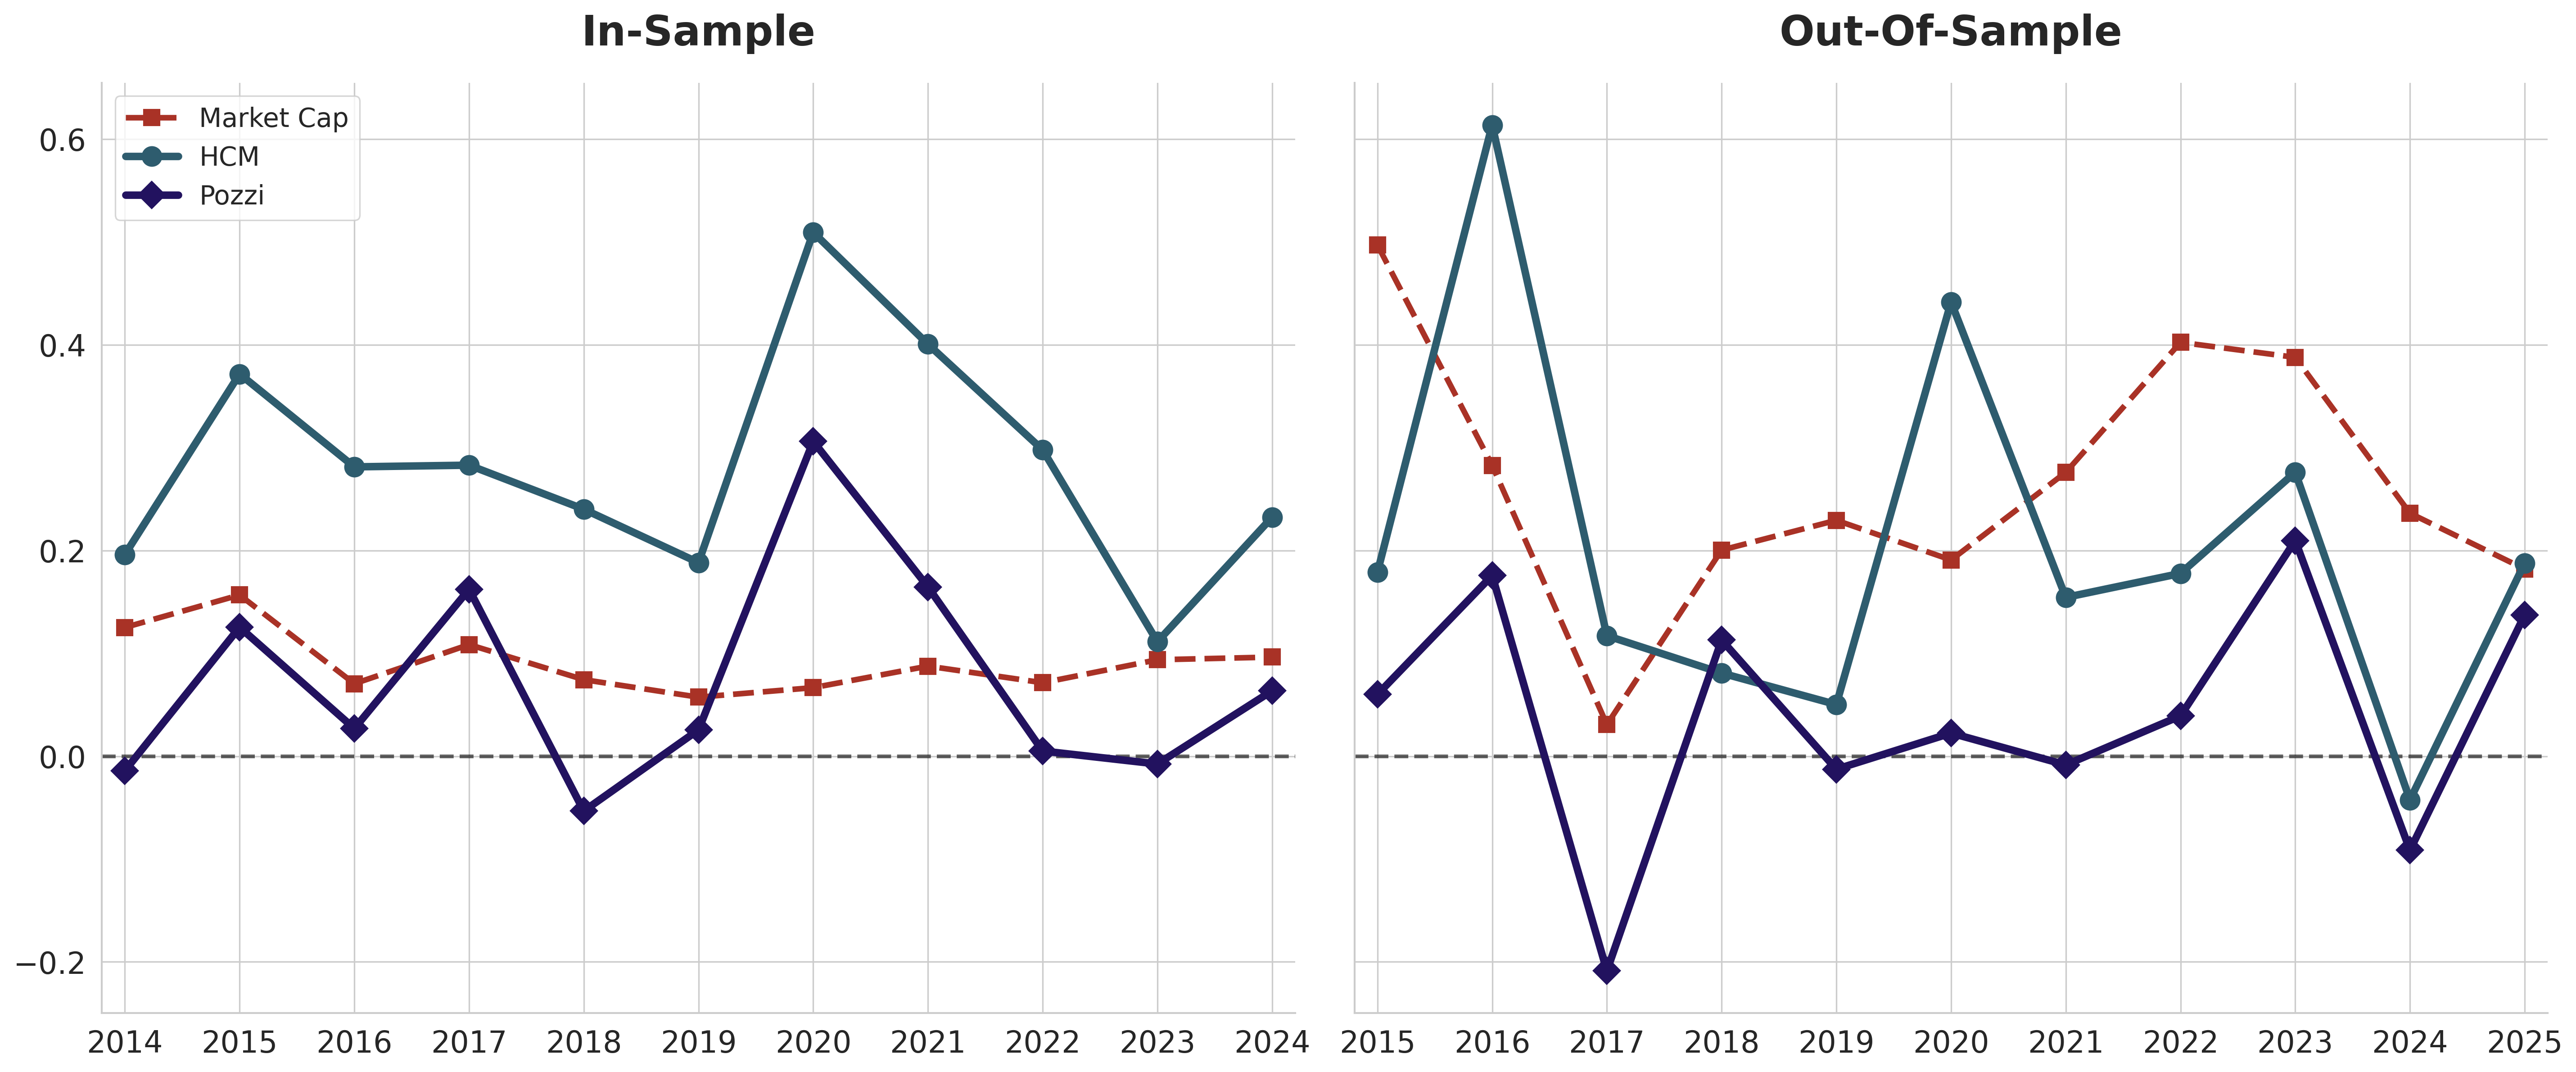
\includegraphics[width=\textwidth]{figures/is_oos_leadlag_comparison.png}
\caption{In-sample Lead--Lag Relationship at left and out-of-sample at right, in respect to both HCM and Pozzi metrics, in the Central to Peripheral direction, and dotted in red the lead-lag relationship by market cap, in the Large to Small direction.}\label{fig:leadlag_insample}
\end{center}
\end{figure}

The in-sample results reveal a stark contrast between the two network methodologies. Under the HCM framework (left panel), the Central $\rightarrow$ Peripheral lead--lag measure is strictly positive and exceptionally strong throughout the entire sample period, peaking significantly around 2020. Crucially, the HCM network-based effect systematically dominates the traditional Big $\rightarrow$ Small size effect. This indicates that the topological hierarchy extracted by HCM captures the true channels of information propagation much more effectively than a simple market capitalization sorting. Conversely, the Pozzi metric (right panel) exhibits high instability. Its lead--lag measure is highly volatile, frequently turning negative (implying the periphery sometimes leads the center), and systematically fails to outperform the traditional size-based benchmark. 

To assess whether these directional dependencies persist in predictive settings, we perform an out-of-sample evaluation using the returns observed during the subsequent year after each network construction, with the results displayed at the right panel in \ref{fig:leadlag_insample}. The out-of-sample evidence demonstrates a significant degradation of the network-derived signal for predictive purposes. When projected into future, unseen data, the traditional Big $\rightarrow$ Small size effect emerges as the most robust and persistent directional force, remaining consistently high across almost all periods. 

For the HCM metric (left panel), while the Central $\rightarrow$ Peripheral relationship remains predominantly positive, it loses its superiority, generally falling below the size-based benchmark and occasionally dipping below zero (e.g., in 2024). This suggests that while HCM perfectly describes the structural information flow of the past, this specific topological advantage partially decays out-of-sample. The Pozzi metric (right panel) performs even worse out-of-sample, exhibiting chaotic, erratic swings.

Overall, the lead--lag analysis highlights the strength of the HCM metric in capturing genuine, superior informational hierarchies within its estimation window. However, the out-of-sample results serve as a reminder of the inherent difficulty in forecasting cross-asset information flows, where the traditional size premium proves to be a more resilient predictor of future lead--lag dynamics than pure correlation-based network topology.

\subsection{Portfolio Performance and Risk Metrics}

\noindent As demonstrated in the lead--lag analysis, the network's topological extremes exhibit fundamentally different information processing speeds, with the highly integrated central core rapidly absorbing market shocks and the disconnected periphery lagging behind. This profound structural dichotomy naturally raises the question of how these informational and risk asymmetries translate into out-of-sample portfolio performance. To investigate this, we evaluate the financial metrics of long-only, buy-and-hold portfolios constructed from the network deciles, rebalanced annually using $1/N$ initial weights. We compare the individual decile portfolios, as well as opposite deciles strategies. The reference benchmark in this section is an equal-weighted ($1/N$), buy-and-hold portfolio of the entire network universe, rebalanced annually, which reflects a naïve diversification strategy rather than the capitalization-weighted market portfolio employed later in the Treynor--Black framework. 

Tables \ref{tab:perf_single} and \ref{tab:perf_union} report the annualized performance and risk metrics—including Compound Annual Growth Rate (CAGR), Volatility, Sharpe Ratio, Maximum Drawdown, and Conditional Value at Risk (CVaR)—for the individual deciles and the opposite deciles strategies, respectively. 

\begin{table}[!htbp]
    % Overrides the rbfin.cls defaults to remove bold text and fix alignments
    \captionsetup{labelfont=normalfont, textfont=normalfont, justification=justified, singlelinecheck=off}
    \centering
    \resizebox{\textwidth}{!}{%
    \begin{tabular}{lcccccccc}
    \toprule
    Strategy & CAGR & Ann. Volatility & Sharpe & Sortino & Max Drawdown & Avg Drawdown & VaR 99\% & CVaR 99\% \\
    \midrule
    Equal-Weighted Universe (1/$N$) & 11.04\% & 15.61\% & 0.75 & 0.93 & -34.34\% & -6.56\% & -2.55\% & -3.98\% \\
    \midrule
    \multicolumn{9}{c}{Panel A: HCM Metric} \\
    \midrule
    Decile 1 (Central) & 8.40\% & 18.26\% & 0.53 & 0.75 & -34.36\% & -7.10\% & -3.14\% & -4.01\% \\
    Decile 2 & 11.57\% & 19.65\% & 0.66 & 0.85 & -40.10\% & -6.04\% & -3.20\% & -4.92\% \\
    Decile 3 & 9.85\% & 18.67\% & 0.60 & 0.75 & -40.92\% & -6.21\% & -3.01\% & -4.76\% \\
    Decile 4 & 9.39\% & 18.01\% & 0.59 & 0.74 & -40.15\% & -6.55\% & -2.89\% & -4.67\% \\
    Decile 5 & 9.47\% & 16.82\% & 0.62 & 0.76 & -39.10\% & -5.90\% & -2.79\% & -4.46\% \\
    Decile 6 & 11.04\% & 17.44\% & 0.69 & 0.86 & -37.36\% & -6.12\% & -2.91\% & -4.50\% \\
    Decile 7 & 11.80\% & 17.22\% & 0.73 & 0.91 & -37.34\% & -7.20\% & -2.93\% & -4.42\% \\
    Decile 8 & 8.00\% & 16.57\% & 0.55 & 0.67 & -37.80\% & -9.18\% & -2.65\% & -4.33\% \\
    Decile 9 & 11.43\% & 15.53\% & 0.77 & 1.03 & -39.49\% & -11.47\% & -2.74\% & -3.82\% \\
    Decile 10 (Peripheral) & 15.12\% & 12.20\% & 1.22 & 1.66 & -30.69\% & -8.85\% & -1.91\% & -2.94\% \\
    \midrule
    \multicolumn{9}{c}{Panel B: Pozzi Metric} \\
    \midrule
    Decile 1 (Central) & 9.75\% & 16.77\% & 0.64 & 0.79 & -39.95\% & -5.44\% & -2.78\% & -4.42\% \\
    Decile 2 & 11.57\% & 16.58\% & 0.74 & 0.93 & -37.15\% & -4.74\% & -2.74\% & -4.30\% \\
    Decile 3 & 8.39\% & 16.61\% & 0.57 & 0.71 & -37.97\% & -6.23\% & -2.66\% & -4.25\% \\
    Decile 4 & 12.52\% & 17.98\% & 0.75 & 0.96 & -35.39\% & -6.39\% & -2.87\% & -4.43\% \\
    Decile 5 & 11.09\% & 17.74\% & 0.68 & 0.85 & -40.59\% & -6.42\% & -2.93\% & -4.57\% \\
    Decile 6 & 8.64\% & 17.77\% & 0.56 & 0.70 & -38.38\% & -8.72\% & -2.86\% & -4.48\% \\
    Decile 7 & 9.95\% & 19.47\% & 0.59 & 0.73 & -39.85\% & -9.31\% & -3.25\% & -5.07\% \\
    Decile 8 & 10.16\% & 16.70\% & 0.66 & 0.89 & -31.09\% & -9.17\% & -2.81\% & -4.00\% \\
    Decile 9 & 8.66\% & 15.41\% & 0.62 & 0.80 & -35.02\% & -12.24\% & -2.64\% & -3.88\% \\
    Decile 10 (Peripheral) & 14.33\% & 16.43\% & 0.90 & 1.25 & -38.12\% & -10.42\% & -2.70\% & -3.71\% \\
    \bottomrule
    \end{tabular}%
    }
    \vspace{0.2cm}
        \caption{Performance and risk metrics for individual decile portfolios. This table reports key financial indicators, including Compound Annual Growth Rate (CAGR), annualized volatility, risk-adjusted returns (Sharpe and Sortino ratios), and tail risk measures (Drawdowns, VaR, and CVaR) across ten network-sorted deciles. All portfolios are evaluated against the equal-weighted ($1/N$), buy-and-hold benchmark of the full network universe reported in the first row. This benchmark differs from the capitalization-weighted market benchmark used in the Treynor--Black analysis and the two should not be compared directly.}
    \label{tab:perf_single}
\end{table}

\begin{table}[!htbp]
    % Overrides the rbfin.cls defaults to remove bold text and fix alignments
    \captionsetup{labelfont=normalfont, textfont=normalfont, justification=justified, singlelinecheck=off}
    \centering
    \resizebox{\textwidth}{!}{%
    \begin{tabular}{lcccccccc}
    \toprule
    Strategy & CAGR & Ann. Volatility & Sharpe & Sortino & Max Drawdown & Avg Drawdown & VaR 99\% & CVaR 99\% \\
    \midrule
    Equal-Weighted Universe (1/$N$) & 11.04\% & 15.61\% & 0.75 & 0.93 & -34.34\% & -6.56\% & -2.55\% & -3.98\% \\
    \midrule
    \multicolumn{9}{c}{Panel A: HCM Metric} \\
    \midrule
    D1 \& D10 & 11.96\% & 13.14\% & 0.93 & 1.26 & -27.21\% & -6.30\% & -2.13\% & -3.02\% \\
    D2 \& D9 & 11.61\% & 16.38\% & 0.75 & 0.97 & -34.67\% & -7.52\% & -2.69\% & -4.07\% \\
    D3 \& D8 & 8.97\% & 17.18\% & 0.59 & 0.72 & -39.34\% & -7.01\% & -2.75\% & -4.45\% \\
    D4 \& D7 & 10.69\% & 17.23\% & 0.68 & 0.84 & -38.74\% & -6.44\% & -2.85\% & -4.49\% \\
    D5 \& D6 & 10.31\% & 16.92\% & 0.67 & 0.82 & -38.10\% & -5.88\% & -2.81\% & -4.44\% \\
    \midrule
    \multicolumn{9}{c}{Panel B: Pozzi Metric} \\
    \midrule
    D1 \& D10 & 12.37\% & 15.27\% & 0.84 & 1.09 & -34.06\% & -5.81\% & -2.48\% & -3.80\% \\
    D2 \& D9 & 10.41\% & 15.00\% & 0.74 & 0.93 & -33.51\% & -6.58\% & -2.52\% & -3.87\% \\
    D3 \& D8 & 9.34\% & 15.89\% & 0.64 & 0.82 & -34.48\% & -6.88\% & -2.57\% & -3.95\% \\
    D4 \& D7 & 11.36\% & 18.07\% & 0.69 & 0.86 & -37.49\% & -7.30\% & -2.97\% & -4.60\% \\
    D5 \& D6 & 9.96\% & 17.29\% & 0.64 & 0.79 & -39.23\% & -7.17\% & -2.76\% & -4.41\% \\
    \bottomrule
    \end{tabular}%
    }
    \vspace{0.2cm}
        \caption{Performance and risk metrics for combined opposite-decile portfolios. This table evaluates the financial performance of opposing strategies constructed by equally weighting symmetrically opposed network deciles. As in Table~\ref{tab:perf_single}, the benchmark is the equal-weighted ($1/N$), buy-and-hold portfolio of the full network universe.}
    \label{tab:perf_union}
\end{table}

An analysis of the individual deciles (Table \ref{tab:perf_single}) reveals that the structural isolation of the periphery acts as a powerful source of risk-adjusted returns. Under the HCM metric, the peripheral portfolio (Decile 10) significantly outperforms the equal-weighted universe benchmark, delivering a CAGR of 15.12\% alongside a remarkably low volatility of 12.20\%, yielding an exceptional Sharpe ratio of 1.22. It also provides the best downside protection across all individual deciles, with a Maximum Drawdown of only -30.69\%. Conversely, the highly integrated central portfolio (Decile 1) underperforms the benchmark, yielding a CAGR of 8.40\% with high volatility (18.26\%) and a poor Sharpe ratio (0.53). This perfectly aligns with our Fama-French pricing error findings: the highly connected core acts as a high-beta market proxy without offering a premium, whereas the idiosyncratic, slow-to-react periphery compensates investors with a substantial structural alpha. The Pozzi metric displays a similar but weaker trend; its peripheral portfolio yields a 14.33\% CAGR but carries much higher volatility (16.43\%) and a worse Maximum Drawdown (-38.12\%), further demonstrating the Pozzi metric's difficulty in cleanly isolating zero-beta assets.

The advantages of the HCM's strict topological separation become even more apparent when deploying the Opposite Deciles strategies (Table \ref{tab:perf_union}). By uniting the extreme core and the extreme periphery (D1 \& D10), investors effectively pair a highly systematic, fast-reacting portfolio with a highly idiosyncratic, delayed-reaction portfolio. This creates massive diversification benefits. Under the HCM metric, the D1 \& D10 portfolio produces a robust CAGR of 11.96\% while compressing annual volatility to just 13.14\% (significantly lower than the benchmark's 15.61\%). Most impressively, this structural pairing limits the Maximum Drawdown to -27.21\% and achieves the lowest VaR and CVaR of any opposite decile strategy. 

However, as the pairings move towards the indistinguishable middle of the network (e.g., D5 \& D6), these topological diversification benefits vanish. The D5 \& D6 portfolio exhibits lower returns (10.31\%), higher volatility (16.92\%), and more pronounced drawdowns (-38.10\%). The Pozzi metric's Opposite Deciles strategies struggle to replicate this level of downside protection, with its D1 \& D10 portfolio suffering a -34.06\% Maximum Drawdown, echoing the metric's instability in predictive settings.

Ultimately, the performance metrics validate the economic implications of the network's structure. The delayed information processing and disconnected nature of the periphery, highlighted in the lead--lag analysis, manifests as an uncorrelated risk premium. When accurately identified by a stable methodology like HCM, pairing this periphery with the market's core creates an exceptionally resilient portfolio that captures the market's directional drift while shielding against systematic drawdowns.

\subsection{Treynor-Black Portfolio}

\noindent\textbf{Implementation Protocol, Rebalancing Turnover, and Friction Analysis}

Before evaluating the gross predictive power of the network signals, it is imperative to quantify the friction introduced by the dynamic reallocation process. We document the two-way portfolio turnover and the subsequent institutional transaction cost drag at each annual rebalancing date. 

Table \ref{tab:turnover} demonstrates that the unconstrained Treynor-Black framework utilizing the Hybrid Centrality Metric (HCM) incurs an average annual portfolio-rebalancing turnover of 96.7\%, translating to a minimal institutional fee drag of 9.7 basis points (bps) per year. Notably, enforcing the Long-Only constraint mitigates extreme idiosyncratic short positions in the central core, reducing turnover by approximately 47\% to an average of 51.4\% (5.1 bps). The Pozzi multiscale centrality metric exhibits marginally higher turnover across both the unconstrained (99.3\%) and Long-Only (53.3\%) implementations, reflecting the previously documented topological instability of this metric. These low transaction costs confirm that the network-derived portfolio weights are structurally persistent and highly investable.

\vskip 2em 
\begin{table}[htbp]
\centering
    \captionsetup{labelfont=normalfont, textfont=normalfont, justification=justified, singlelinecheck=off}
\begin{tabular}{@{}lcccc@{}}
\toprule
Portfolio & Turnover (\%) & Cost (bps) \\ \midrule
HCM Unconstrained & 96.7\% & 9.7 \\
HCM Long-Only & 51.4\% & 5.1 \\
Pozzi Unconstrained & 99.3\% & 9.9 \\
Pozzi Long-Only & 53.3\% & 5.3 \\ \bottomrule
\end{tabular}
\vskip 1em
\caption{Dynamic Portfolio Rebalancing Turnover and Transaction Cost Drag (10-Year Mean)}
\label{tab:turnover}
\end{table}

\vskip 2em
\noindent\textbf{Out-of-Sample Performance and Downside Risk Profile}
Figure \ref{fig:cum_returns} and Table \ref{tab:performance_metrics} delineate the cumulative wealth paths, drawdown profiles and overall risk-return profile of the evaluated strategies relative to the capitalization-weighted market benchmark (i.e., the value-weighted portfolio of the full network universe, as defined in Section~\ref{sec:methodology}). This benchmark is deliberately distinct from the equal-weighted ($1/N$), buy-and-hold universe benchmark used in the preceding performance analysis, and the two are not directly comparable. Over the out-of-sample horizon (2015–2024), the benchmark generated a Compound Annual Growth Rate (CAGR) of 20.96\% with an annualized volatility of 18.42\% and a Maximum Drawdown of -34.28\%. All metrics in this section are computed over the 2015--2024 out-of-sample window; the 2014 warm-up year is excluded.

\begin{figure}[htbp]
    \centering
    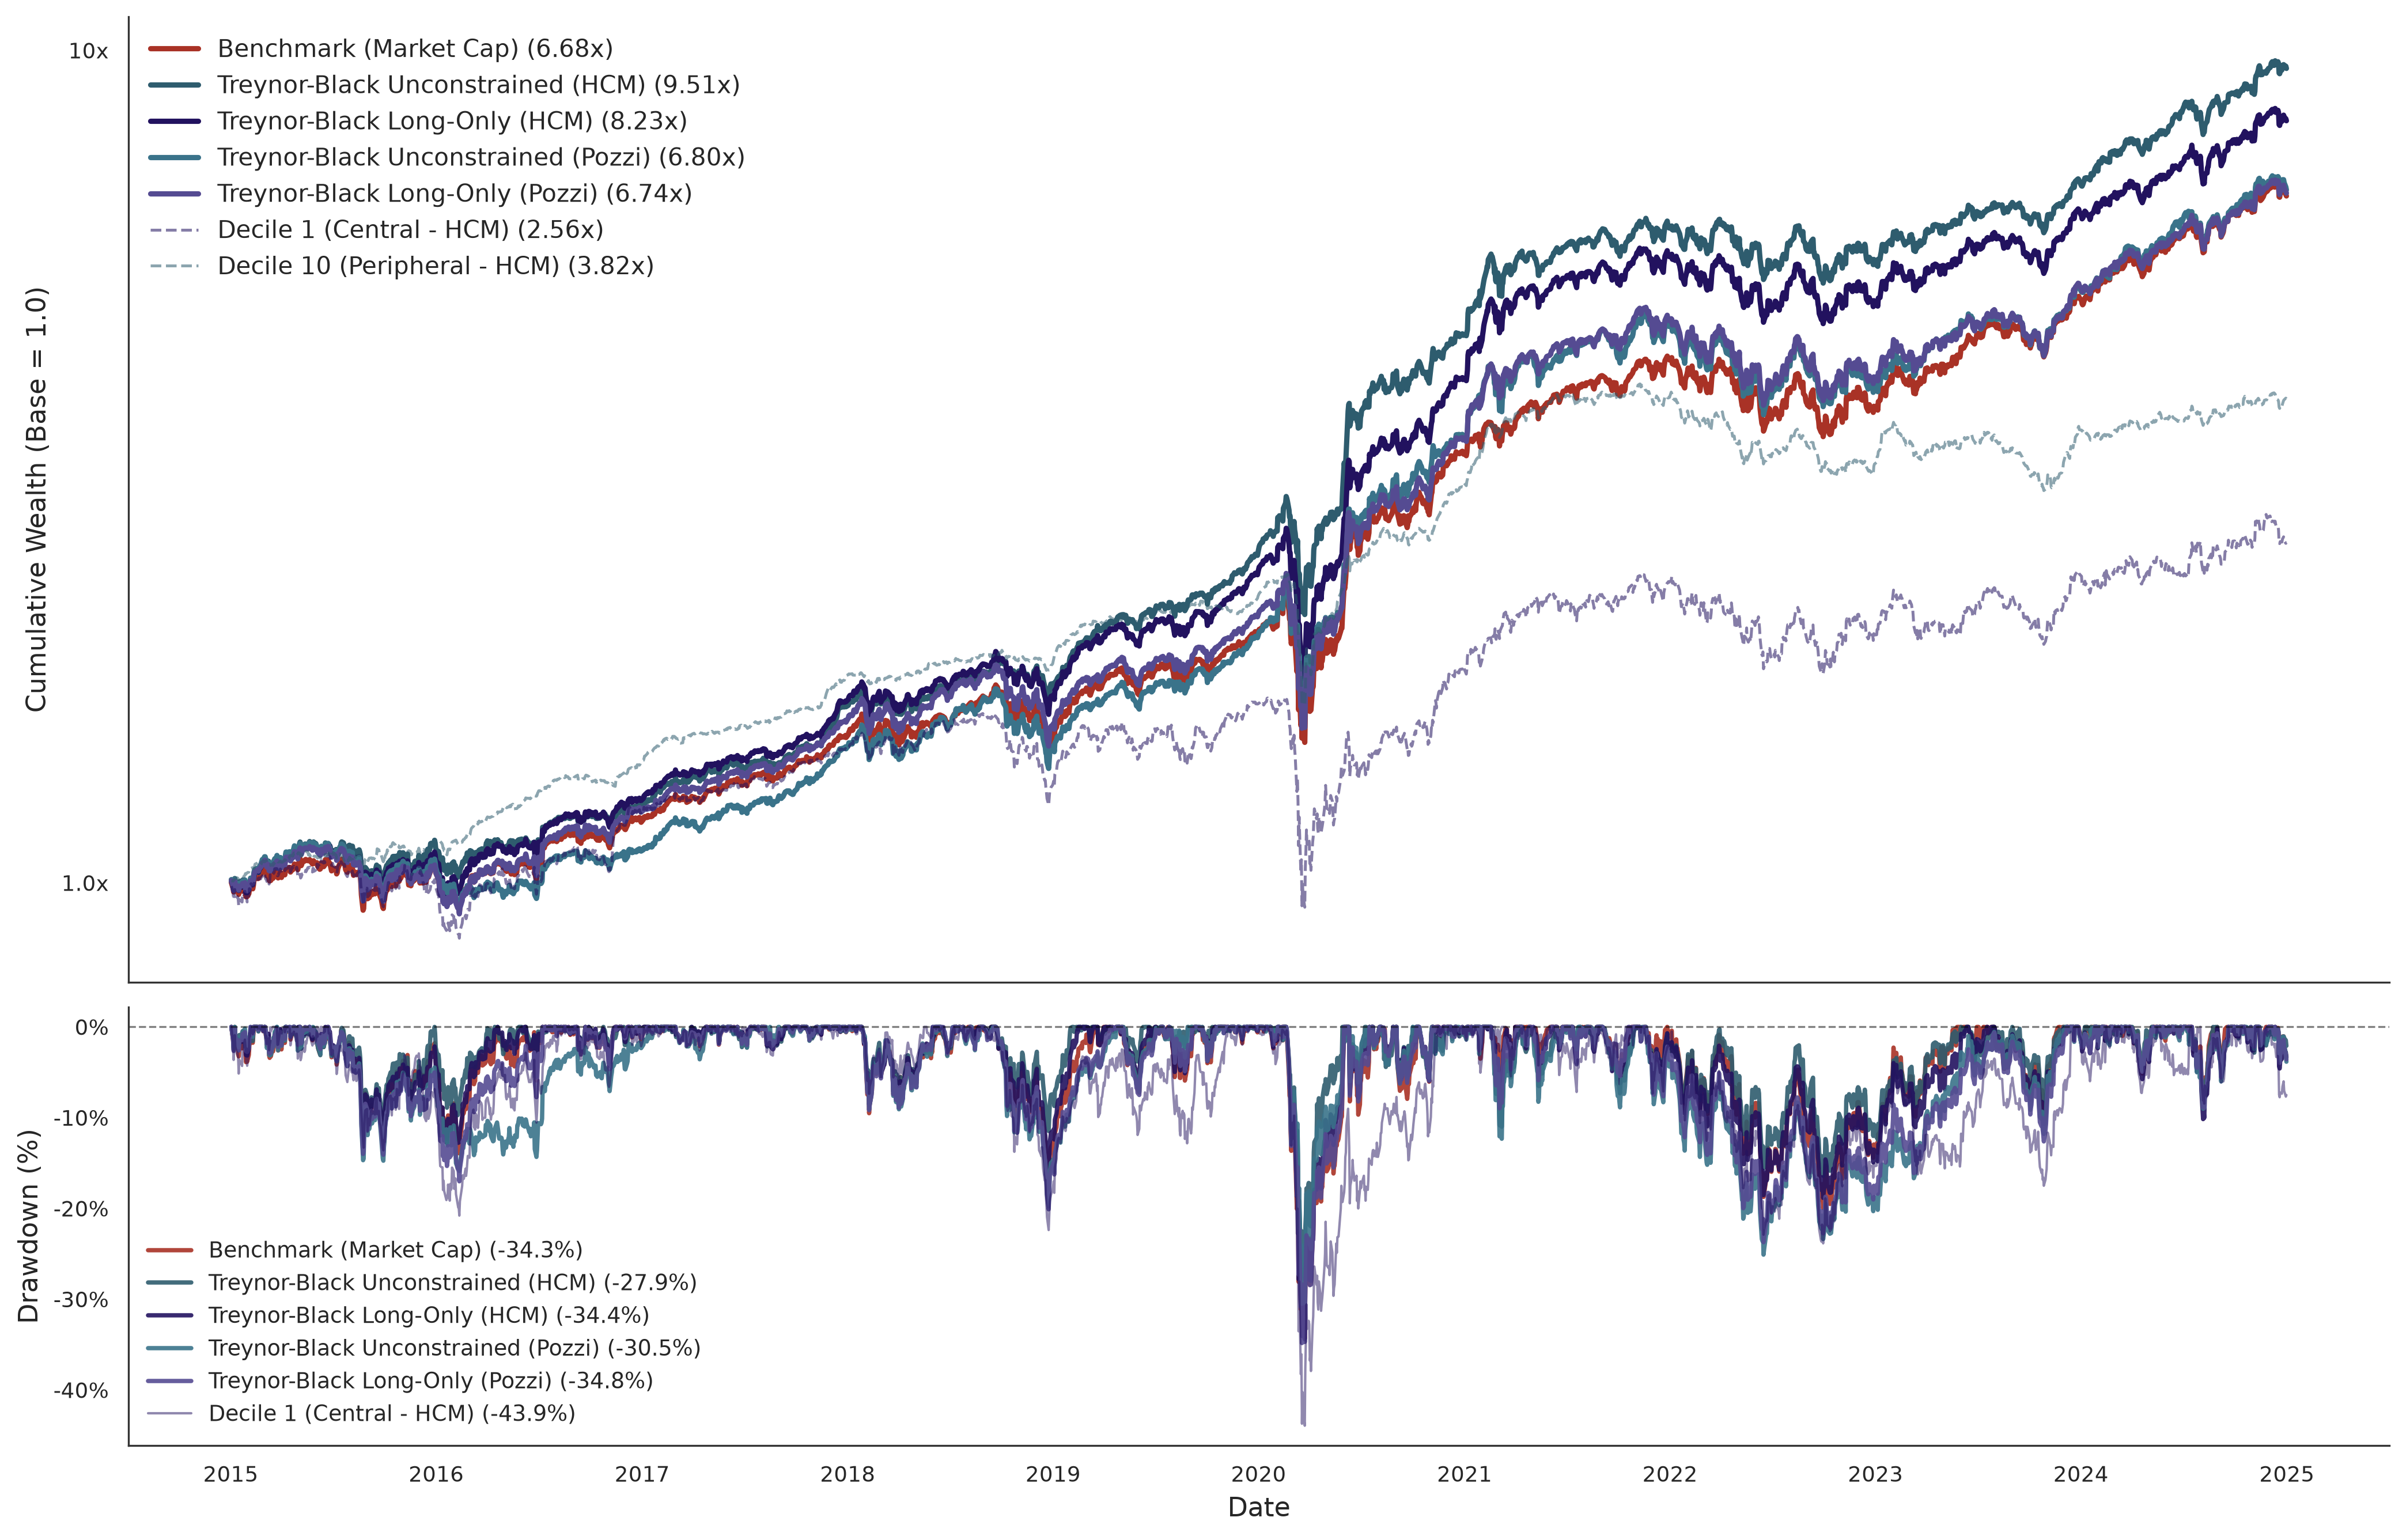
\includegraphics[width=\textwidth]{figures/shared/01_cum_returns_drawdowns.png}
    \caption{Out-of-Sample Cumulative Returns and Drawdown Profiles (2015--2024)}
    \label{fig:cum_returns}
\end{figure}

\begin{table}[htbp]
\centering
\captionsetup{labelfont=normalfont, textfont=normalfont, justification=justified, singlelinecheck=off}
\resizebox{\textwidth}{!}{
\begin{tabular}{@{} l *{19}{c} @{}}
\toprule
Strategy & Total Ret. & CAGR & Ann. Vol. & Sharpe & Sortino & Max Drawdown & Calmar & 95\% VaR & 95\% CVaR \\ \midrule
Benchmark (Market Cap) & 568.50\% & 20.96\% & 18.42\% & 1.13 & 1.64 & -34.28\% & 0.61 & -1.63\% & -2.67\% \\
Treynor-Black Unc. (HCM) & 851.25\% & 25.31\% & 16.36\% & 1.46 & 2.21 & -27.85\% & 0.91 & -1.49\% & -2.32\% \\
Treynor-Black LO (HCM) & 723.14\% & 23.51\% & 17.60\% & 1.29 & 1.88 & -34.42\% & 0.68 & -1.56\% & -2.53\% \\
Treynor-Black Unc. (Pozzi) & 579.71\% & 21.16\% & 18.41\% & 1.14 & 1.66 & -30.50\% & 0.69 & -1.74\% & -2.64\% \\
Treynor-Black LO (Pozzi) & 573.74\% & 21.05\% & 18.22\% & 1.14 & 1.65 & -34.83\% & 0.60 & -1.63\% & -2.63\% \\
\bottomrule
\end{tabular}
}
\vskip 1em
\caption{Out-of-Sample Performance and Downside Risk Metrics (2015--2024). The benchmark is the capitalization-weighted market portfolio of the full network universe. It is intentionally different from the equal-weighted ($1/N$) universe benchmark used in Tables~\ref{tab:perf_single}--\ref{tab:perf_union}. VaR and CVaR are expressed as losses (negative values).}
\label{tab:performance_metrics}
\end{table}

The Treynor-Black optimization successfully exploits the structural asymmetry between the central and peripheral network deciles. The HCM Unconstrained strategy significantly outperforms, delivering a CAGR of 25.31\%, suppressing volatility to 16.36\%, and reducing the Maximum Drawdown to -27.85\%. This yields a superior Sharpe ratio of 1.46 and a Sortino ratio of 2.21, compared to the benchmark's 1.13 and 1.64, respectively. The HCM Long-Only strategy maintains robust outperformance with a 23.51\% CAGR and a Sharpe ratio of 1.29. Consistent with our topological stability analysis, the Pozzi metric provides less efficient signal translation. The Pozzi Unconstrained strategy yields a 21.16\% CAGR (Sharpe 1.14), only marginally beating the benchmark, while suffering a -30.50\% drawdown.

\vskip2em
\noindent\textbf{Sector Tilts}

To contextualize the drivers of risk-adjusted outperformance, we examine the micro-level portfolio holdings and dynamic active sector tilts ($\Delta w = w_p - w_M$) generated by each optimization framework. Figures \ref{fig:sector_tilts_unc_hcm} and \ref{fig:sector_tilts_lo_hcm} map these active macroeconomic exposures over the out-of-sample decade for the HCM metric.

\begin{figure}[htbp]
    \centering
    \captionsetup{labelfont=normalfont, textfont=normalfont, justification=justified, singlelinecheck=off}
    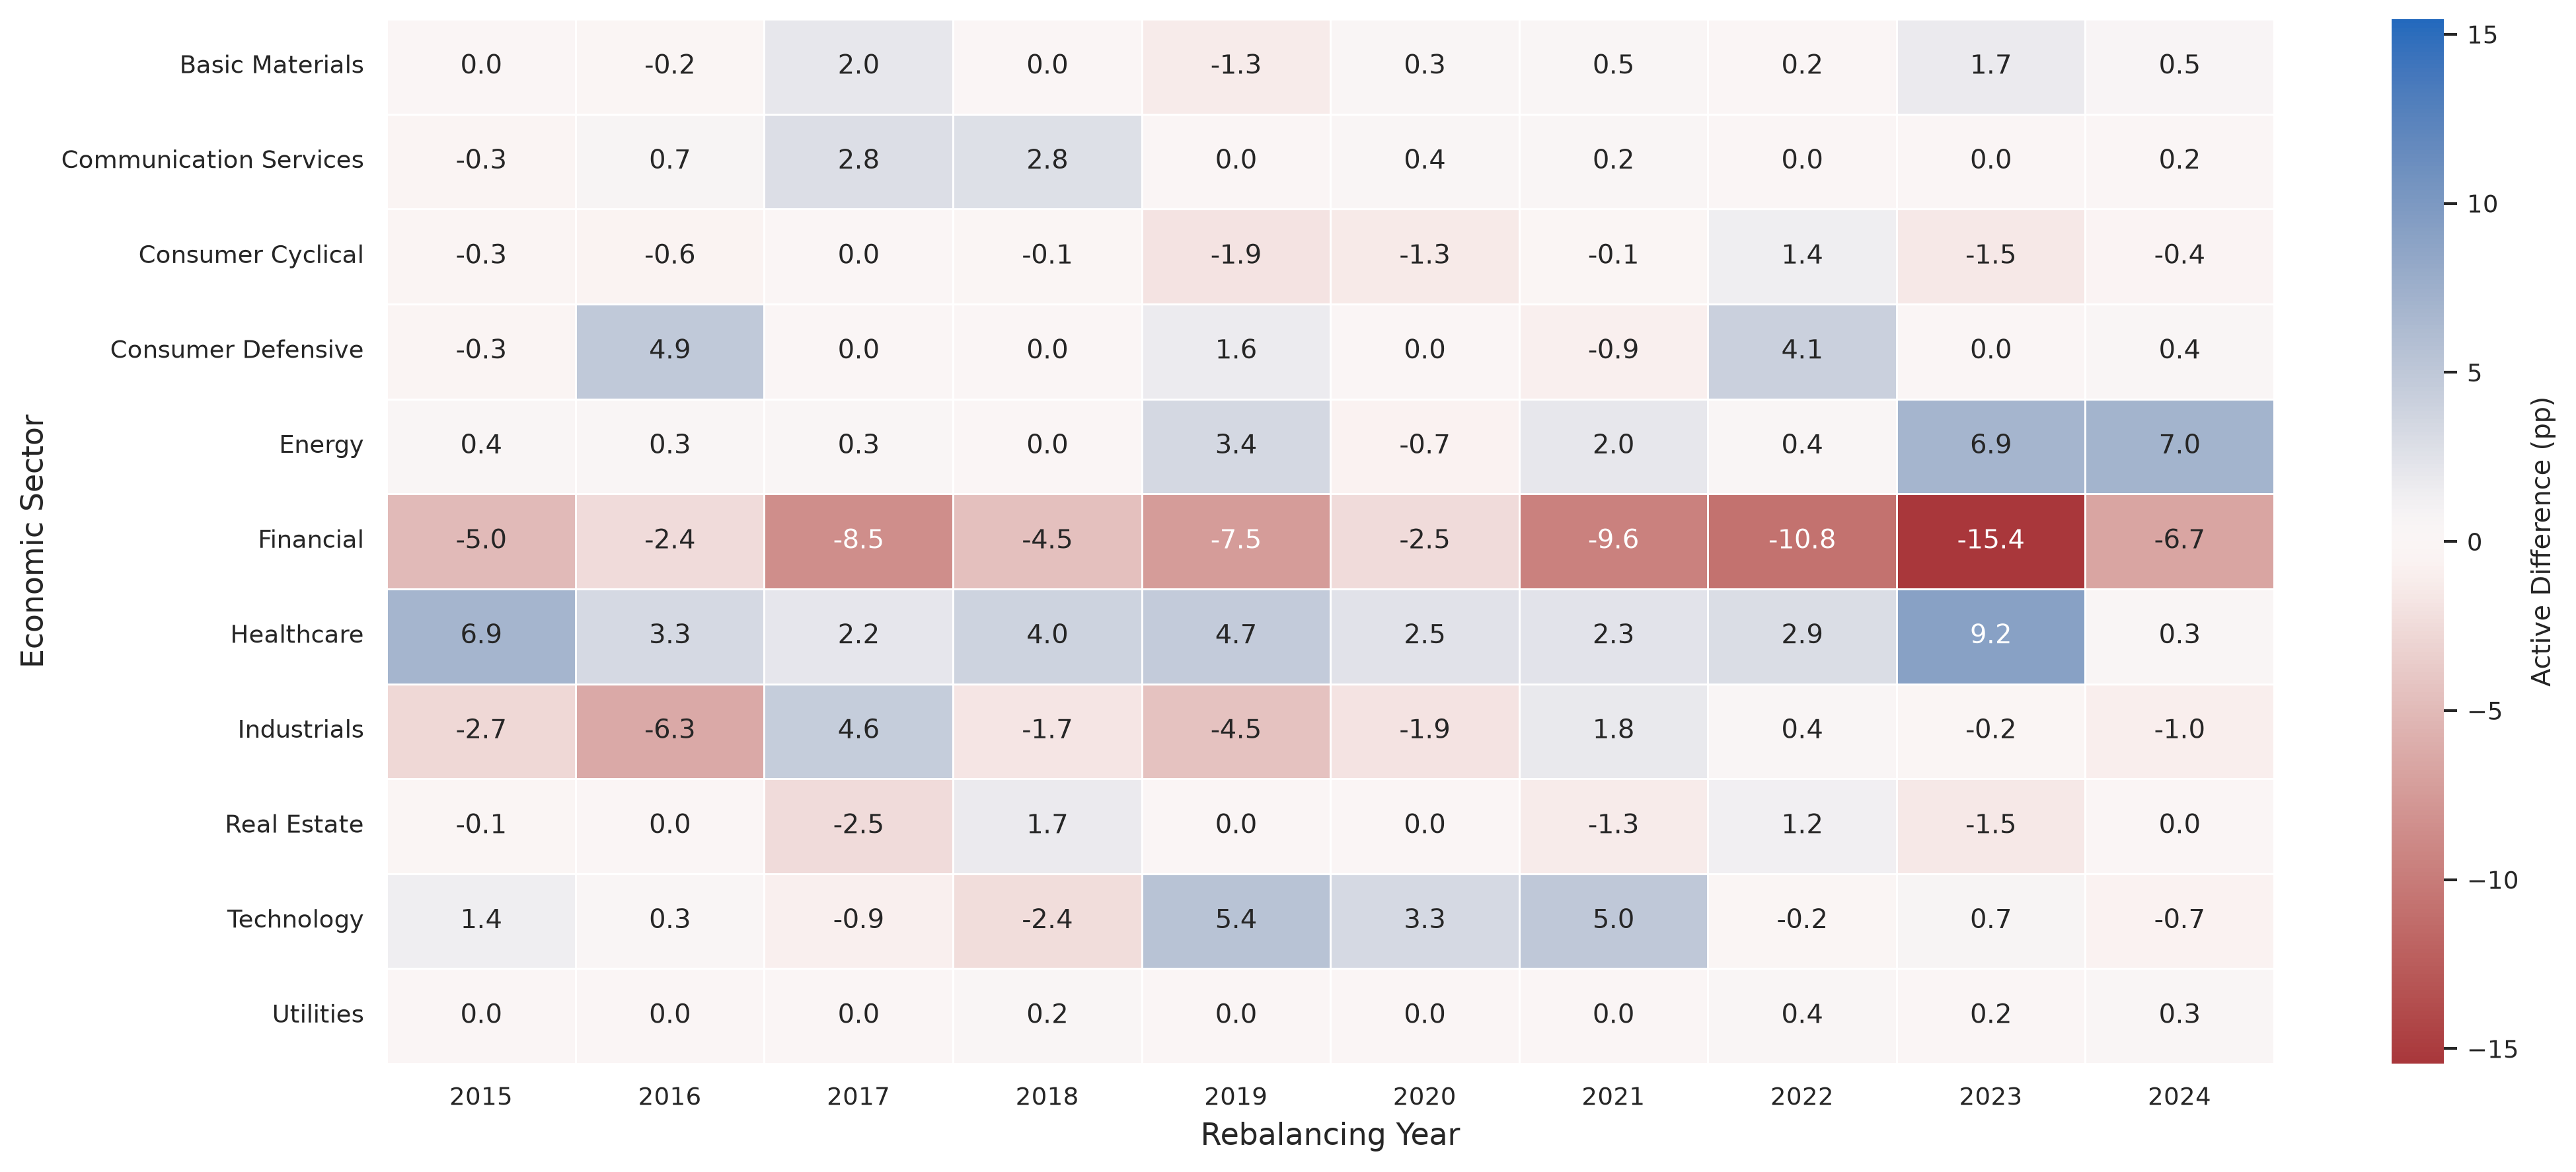
\includegraphics[width=\textwidth]{figures/hcm/05_sector_tilts_unconstrained_hcm.png}
    \caption{Active Sector Tilts: Treynor-Black Unconstrained (HCM)}
    \label{fig:sector_tilts_unc_hcm}
\end{figure}

\begin{figure}[htbp]
    \centering
    \captionsetup{labelfont=normalfont, textfont=normalfont, justification=justified, singlelinecheck=off}
    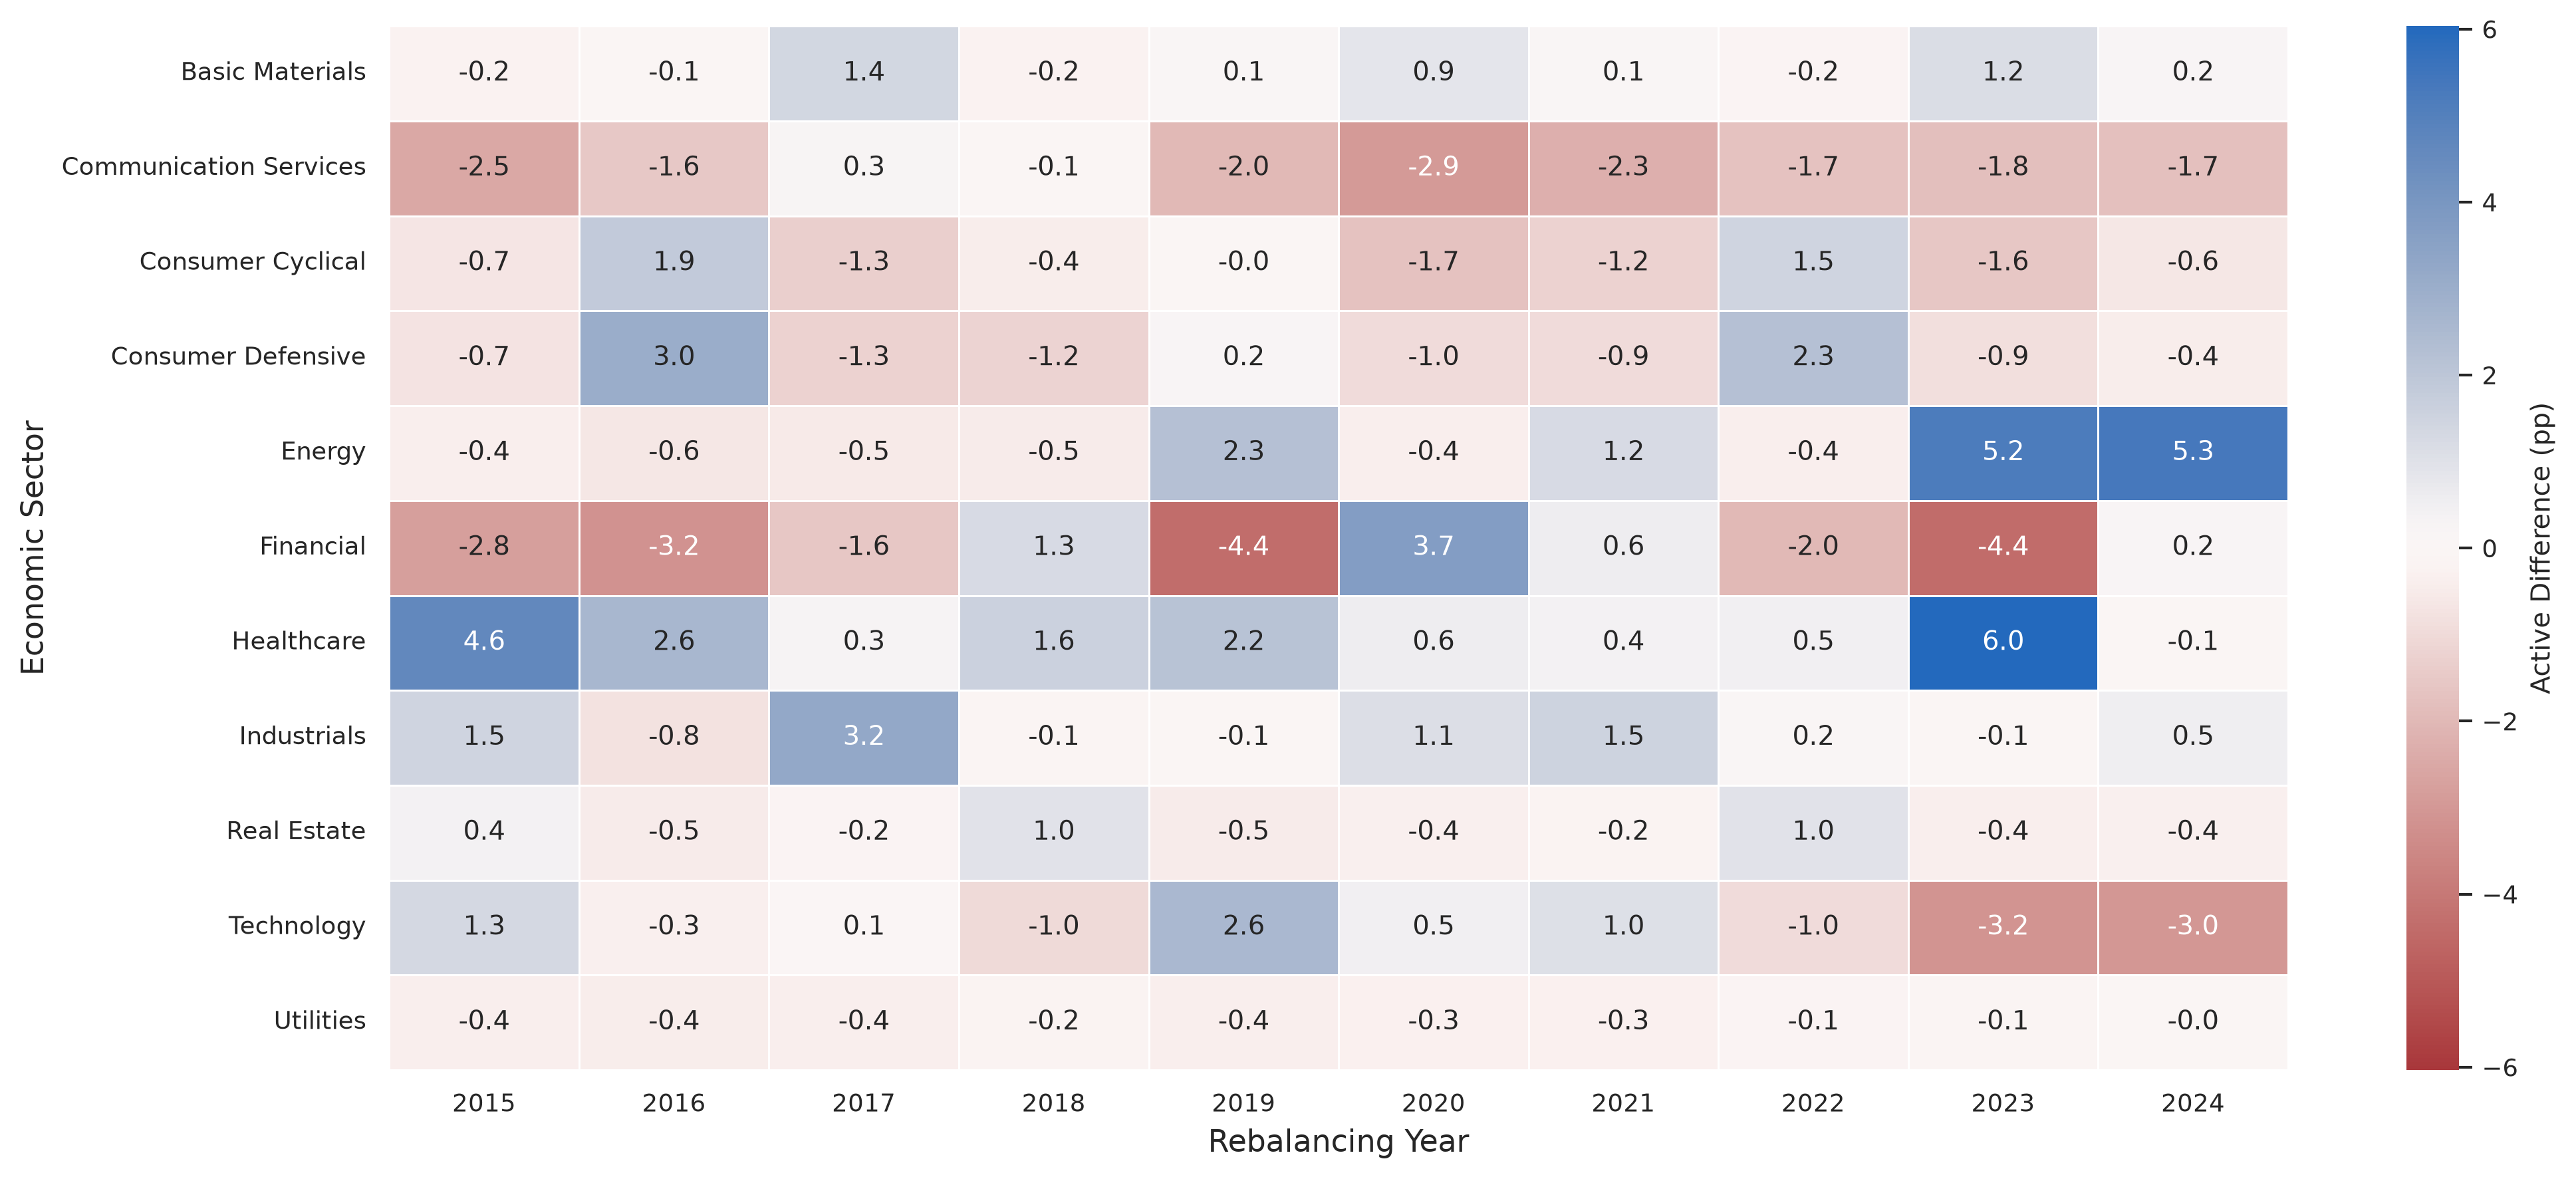
\includegraphics[width=\textwidth]{figures/hcm/06_sector_tilts_long_only_hcm.png}
    \caption{Active Sector Tilts: Treynor-Black Long-Only (HCM)}
    \label{fig:sector_tilts_lo_hcm}
\end{figure}

The Treynor-Black Unconstrained framework utilizing the HCM (Figure \ref{fig:sector_tilts_unc_hcm}) demonstrates a remarkably stable, economically intuitive structural thesis. By mathematically identifying Financials and Industrials as the highly integrated systematic core, the strategy persistently funds its active bets by underweighting these sectors—most notably stripping up to 15.4 percentage points of active weight from Financials in 2023. This capital is systematically redirected toward idiosyncratic, peripheral sectors such as Healthcare and Energy. Imposing the Long-Only constraint on the HCM metric (Figure \ref{fig:sector_tilts_lo_hcm}) naturally truncates the deep negative active weights in the central core by prohibiting short sales. Consequently, the sector tilts are significantly attenuated. Rather than heavily shorting the financial core, the strategy scales back its active deviations, achieving a tighter tracking error while preserving targeted structural overweights in peripheral conduits, such as a +6.0 percentage point tilt toward Healthcare in 2023.

In stark contrast, the multiscale Pozzi centrality metric fails to establish a persistent macroeconomic topology. Its unconstrained strategy exhibits erratic regime shifts that align with its previously documented high turnover rates: a massive -18.0 percentage point underweight to Financials in 2015 reverses to a +8.6 percentage point overweight by 2024, and its active Healthcare exposure oscillates from +16.2 percentage points in 2023 to -6.4 percentage points the following year. The long-only formulation suppresses the magnitude of these swings but not the underlying year-over-year rotation. We report the sector tilts for HCM only; the Pozzi analogues are available in the replication package.

\vskip2em
\noindent\textbf{Factor Attribution and Market Risk Reduction} We formally evaluate the origins of the active returns using Fama-French 3-Factor regressions (Table \ref{tab:fama_french}), deploying Newey-West HAC standard errors \citep{newey1987} to ensure robustness. The analysis confirms that the excess returns generated by the network-derived strategies are not spanned by traditional market, size (SMB), or value (HML) risk premia, although Section~\ref{sec:robustness} shows that they are partly related to size and low-beta exposures.

The HCM Unconstrained strategy produces an annualized Jensen's alpha of +12.72\% ($t=4.42$) while driving its systematic market beta down to 0.755 from the benchmark's 0.936. This is a concentrated-strategy result rather than a diversified premium: the overlay holds at most 25 long and 25 short positions, with an active share of about 20\%, and its magnitude is not adjusted for the on-sample design search (Section~\ref{sec:robustness}). The unconstrained overlay loads negatively on the Value factor ($-0.084$, $t=-3.59$) and the Size factor ($-0.070$, $t=-1.99$); the long-only variant shifts the SMB loading to $+0.111$ ($t=4.05$) and preserves an alpha of $+10.69\%$ ($t=4.48$). The adjusted $R^2$ falls to 70.92\% from the benchmark's 86.36\%, confirming that the strategy decouples from the broad market.

Conversely, the multiscale Pozzi centrality metric demonstrates a diminished capacity to isolate pure topological alpha. While the Pozzi Unconstrained strategy generates a statistically significant alpha of +8.29\% ($t=2.90$), it retains a higher market beta of 0.871 and a strong negative exposure to the HML factor ($-0.144$, $t=-5.92$). Interestingly, the Pozzi Long-Only variant yields a nearly identical alpha of +8.35\% ($t=3.61$) alongside an elevated market beta of 0.904 and a pronounced positive loading on the SMB factor (0.144, $t=5.16$). Ultimately, these regressions confirm that the HCM metric's core-periphery separation is more effective than the Pozzi framework at neutralizing systematic market exposure and isolating factor-adjusted alpha.

\vskip 1em
\begin{table}[htbp]
\centering
\captionsetup{labelfont=normalfont, textfont=normalfont, justification=justified, singlelinecheck=off}
\resizebox{\textwidth}{!}{
\begin{tabular}{@{}lccccc@{}}
\toprule
Parameter & Benchmark & HCM Unc. & HCM LO & Pozzi Unc. & Pozzi LO\\ \midrule
Annualized Alpha (\%) & 7.79\% & 12.72\% & 10.69\% & 8.29\% & 8.35\% \\
$t$-statistic & (3.45) & (4.42) & (4.48) & (2.90) & (3.61) \\
Market Beta & 0.936 & 0.755 & 0.866 & 0.871 & 0.904 \\
$t$-statistic & (88.11) & (49.51) & (70.25) & (60.95) & (85.64) \\
Size Beta (SMB) & 0.022 & -0.070 & 0.111 & 0.019 & 0.144\\
Value Beta (HML) & 0.041 & -0.084 & 0.030 & -0.144 & 0.015\\
Adjusted $R^2$ (\%) & 86.36\% & 70.92\% & 83.38\% & 77.46\% & 85.70\% \\ \bottomrule
\end{tabular}}
\vskip 1em
\caption{Fama-French 3-Factor Regressions}
\label{tab:fama_french}
\end{table}

\noindent These active results should be read jointly with the robustness analysis of Section~\ref{sec:robustness}: the overlay concentrates on the 25 highest-alpha names in each extreme decile and shorts the core, so its alpha is not spanned by the market, size and value factors, while the underlying peripheral premium is concentrated in small caps, carries a positive betting-against-beta loading, and weakens once exchange-traded funds are removed. The active outperformance therefore combines network-based selection with these known effects rather than constituting a purely topological anomaly.

The result is robust to the two discretionary design choices. Table~\ref{tab:tb_sensitivity} reports the annualized FF3 alpha across the top-$k$ screen ($k\in\{10,25,50\}$) and the active budget ($10\%,20\%,30\%$): it remains between $+8.7\%$ and $+20.9\%$ (all $t>3.6$) and is monotone in both parameters. We use the conservative $k=25$, $w_A=20\%$ specification throughout. Because the overlay's design was selected on the same sample, this strategy-level alpha is not adjusted for design multiplicity, whereas the decile-level premium is (Section~\ref{sec:robustness}). The Pozzi overlay behaves similarly (FF3 alpha between $+7.9\%$ and $+12.1\%$ across the same grid, all $t>2.4$), and starting the performance window in 2016 leaves the HCM unconstrained alpha essentially unchanged ($+13.3\%$, $t=4.32$).

\begin{table}[htbp]
\centering
\captionsetup{labelfont=normalfont, textfont=normalfont, justification=justified, singlelinecheck=off}
\caption{Sensitivity of the HCM unconstrained strategy to the top-$k$ alpha screen and the active budget $w_A$. Entries are annualized FF3 (Newey--West) alphas in percent, with $t$-statistics in parentheses; the out-of-sample window is 2015--2024.}
\label{tab:tb_sensitivity}
\begin{tabular}{lccc}
\toprule
Active budget $w_A$ & $k=10$ & $k=25$ & $k=50$ \\
\midrule
10\% & 12.16 (4.58) & 10.24 (4.20) & 8.65 (3.69) \\
20\% & 16.55 (4.66) & 12.72 (4.42) & 9.54 (3.74) \\
30\% & 20.94 (4.49) & 15.20 (4.38) & 10.43 (3.66) \\
\bottomrule
\end{tabular}
\end{table}

\vskip 2em
\noindent\textbf{Capital Allocation Line} Finally, we assess the broader institutional applicability of the network topology by constructing convex combinations of the equity strategies with the risk-free asset (Figures \ref{fig:cal}, \ref{fig:blends_unc_hcm}, and \ref{fig:blends_lo_hcm} and Table \ref{tab:cal_blends}). Figure \ref{fig:cal} illustrates the outward shift of the Capital Allocation Line (CAL). The standard market benchmark defines a baseline CAL with a Sharpe slope of 1.03. The HCM Unconstrained framework pushes this efficient frontier outward to a Sharpe slope of 1.36, dominating the market benchmark over the relevant range of volatilities.

\begin{figure}[htbp]
    \centering
    \captionsetup{labelfont=normalfont, textfont=normalfont, justification=justified, singlelinecheck=off}
    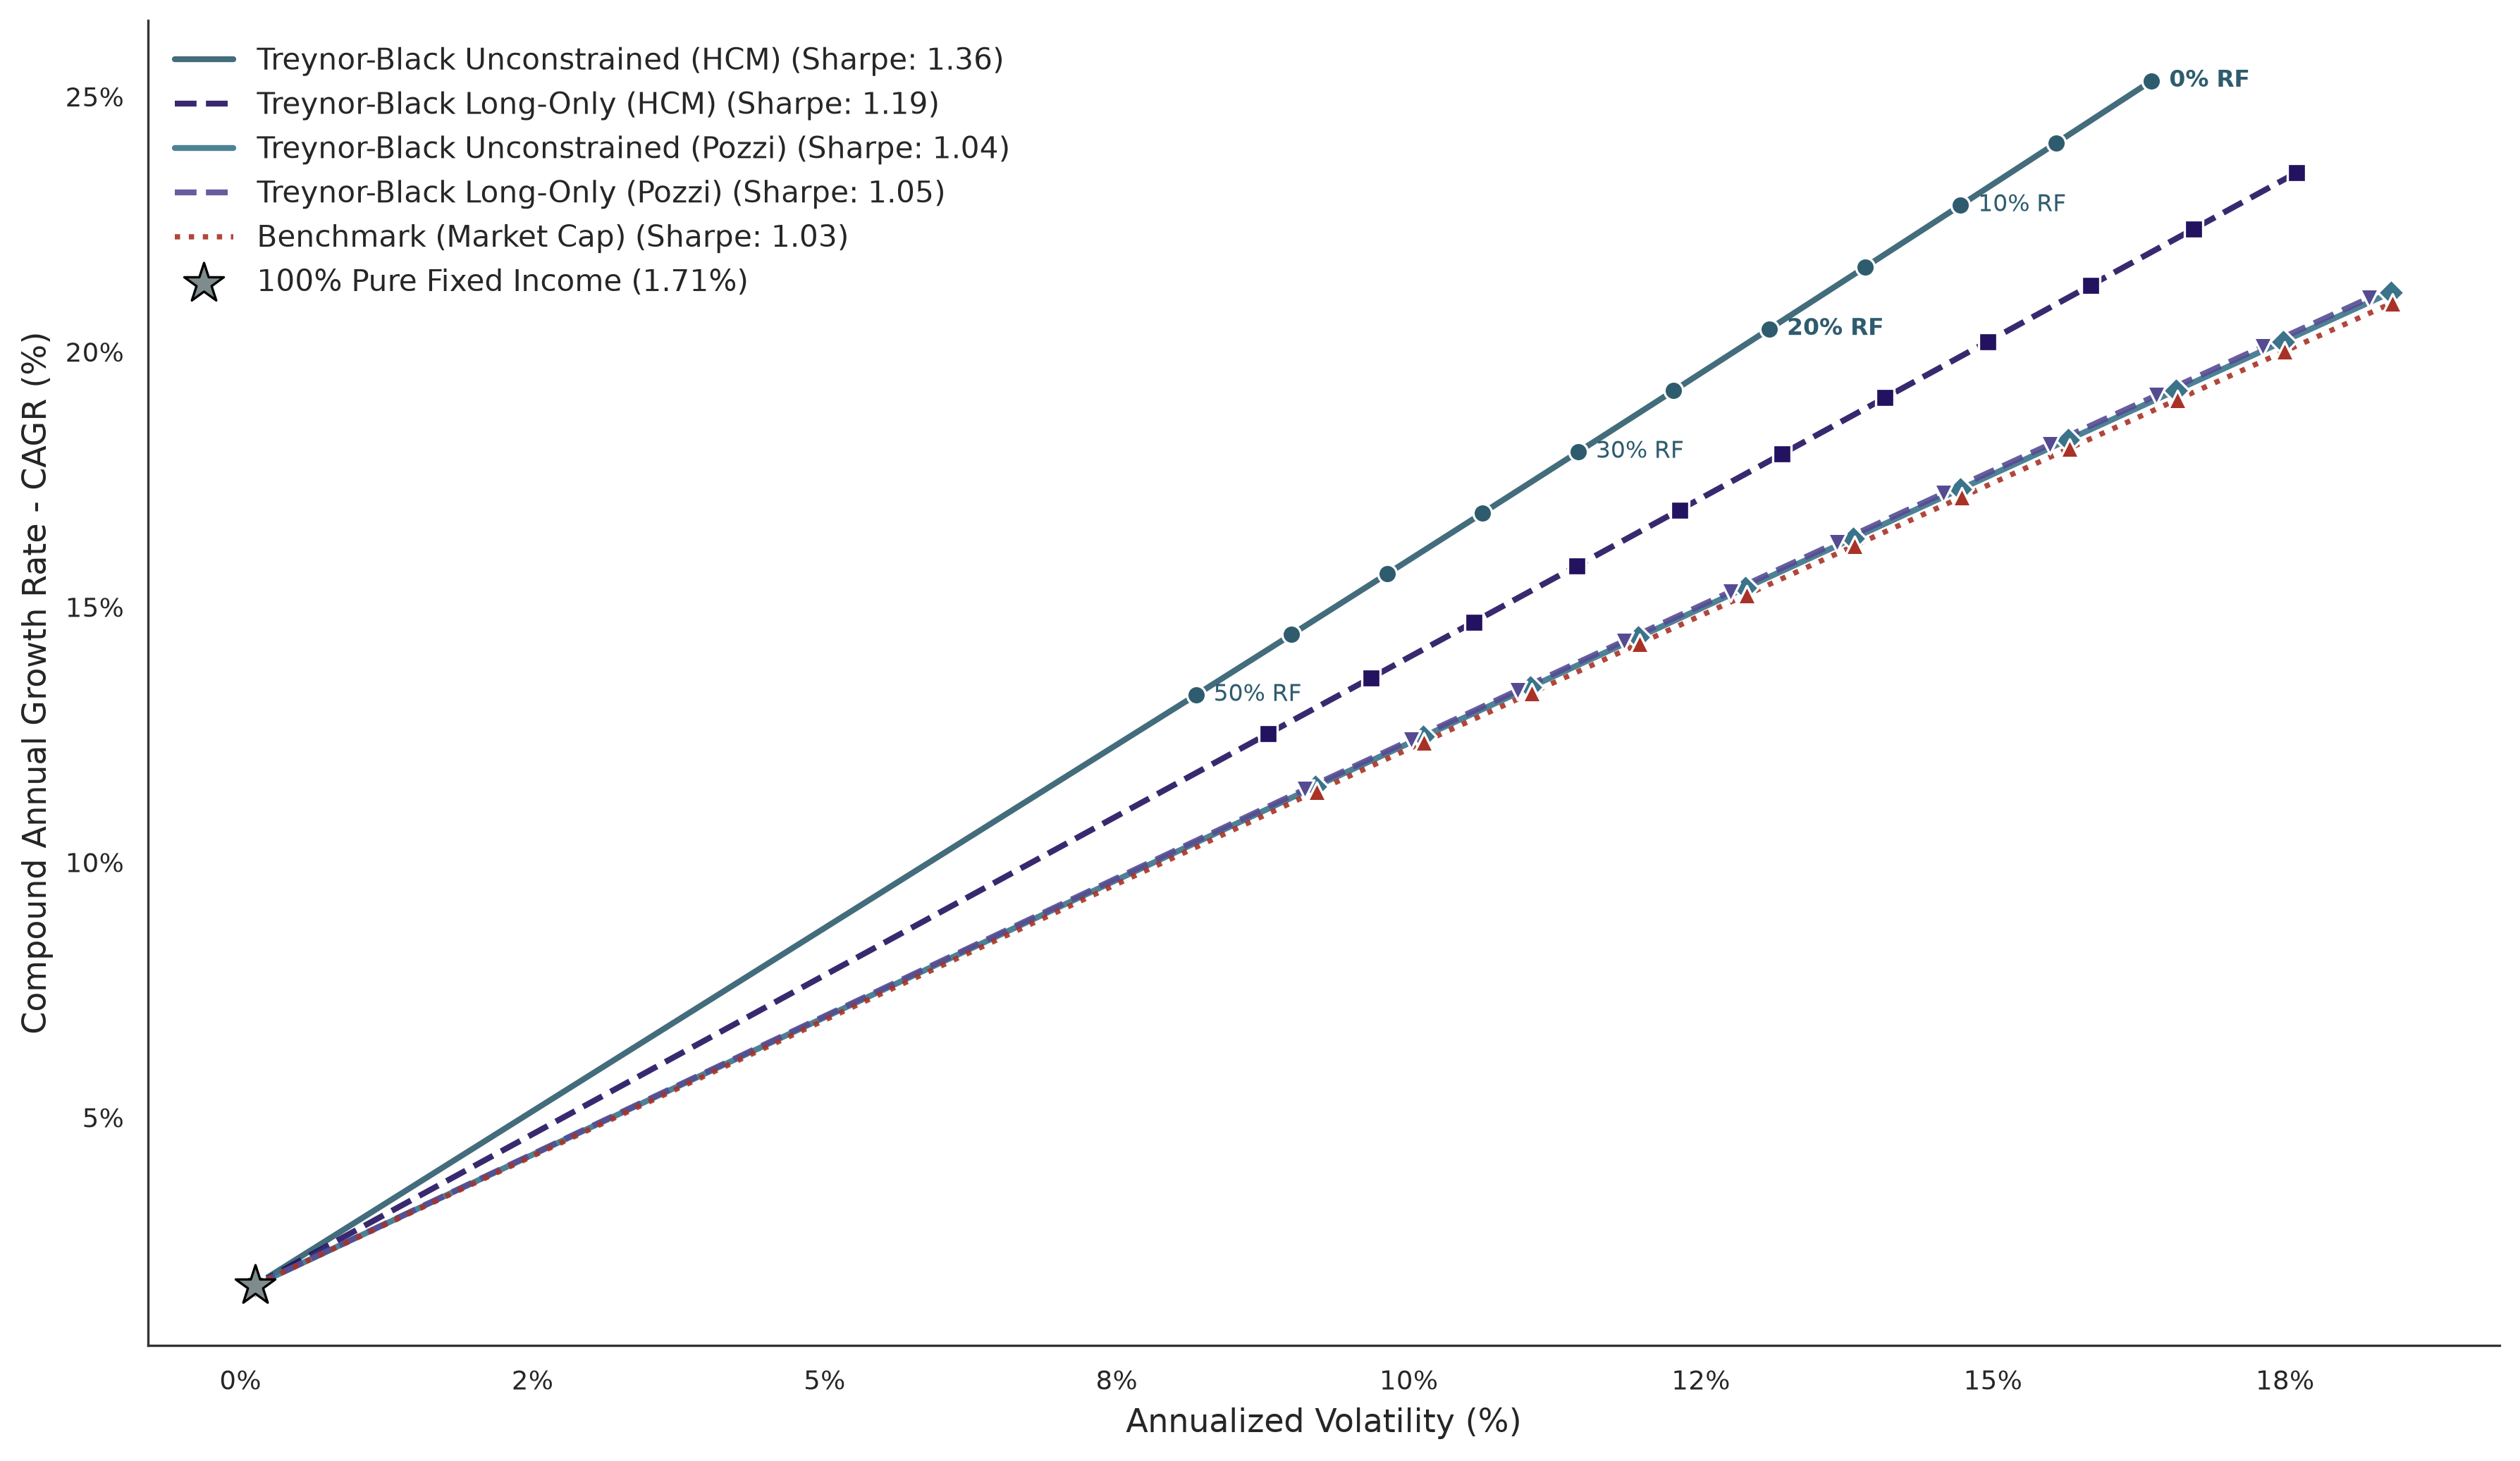
\includegraphics[width=\textwidth]{figures/shared/12_efficient_frontier_cal.png}
    \caption{Capital Allocation Line and Efficient Frontier}
    \label{fig:cal}
\end{figure}

\begin{figure}[htbp]
    \centering
    \captionsetup{labelfont=normalfont, textfont=normalfont, justification=justified, singlelinecheck=off}
    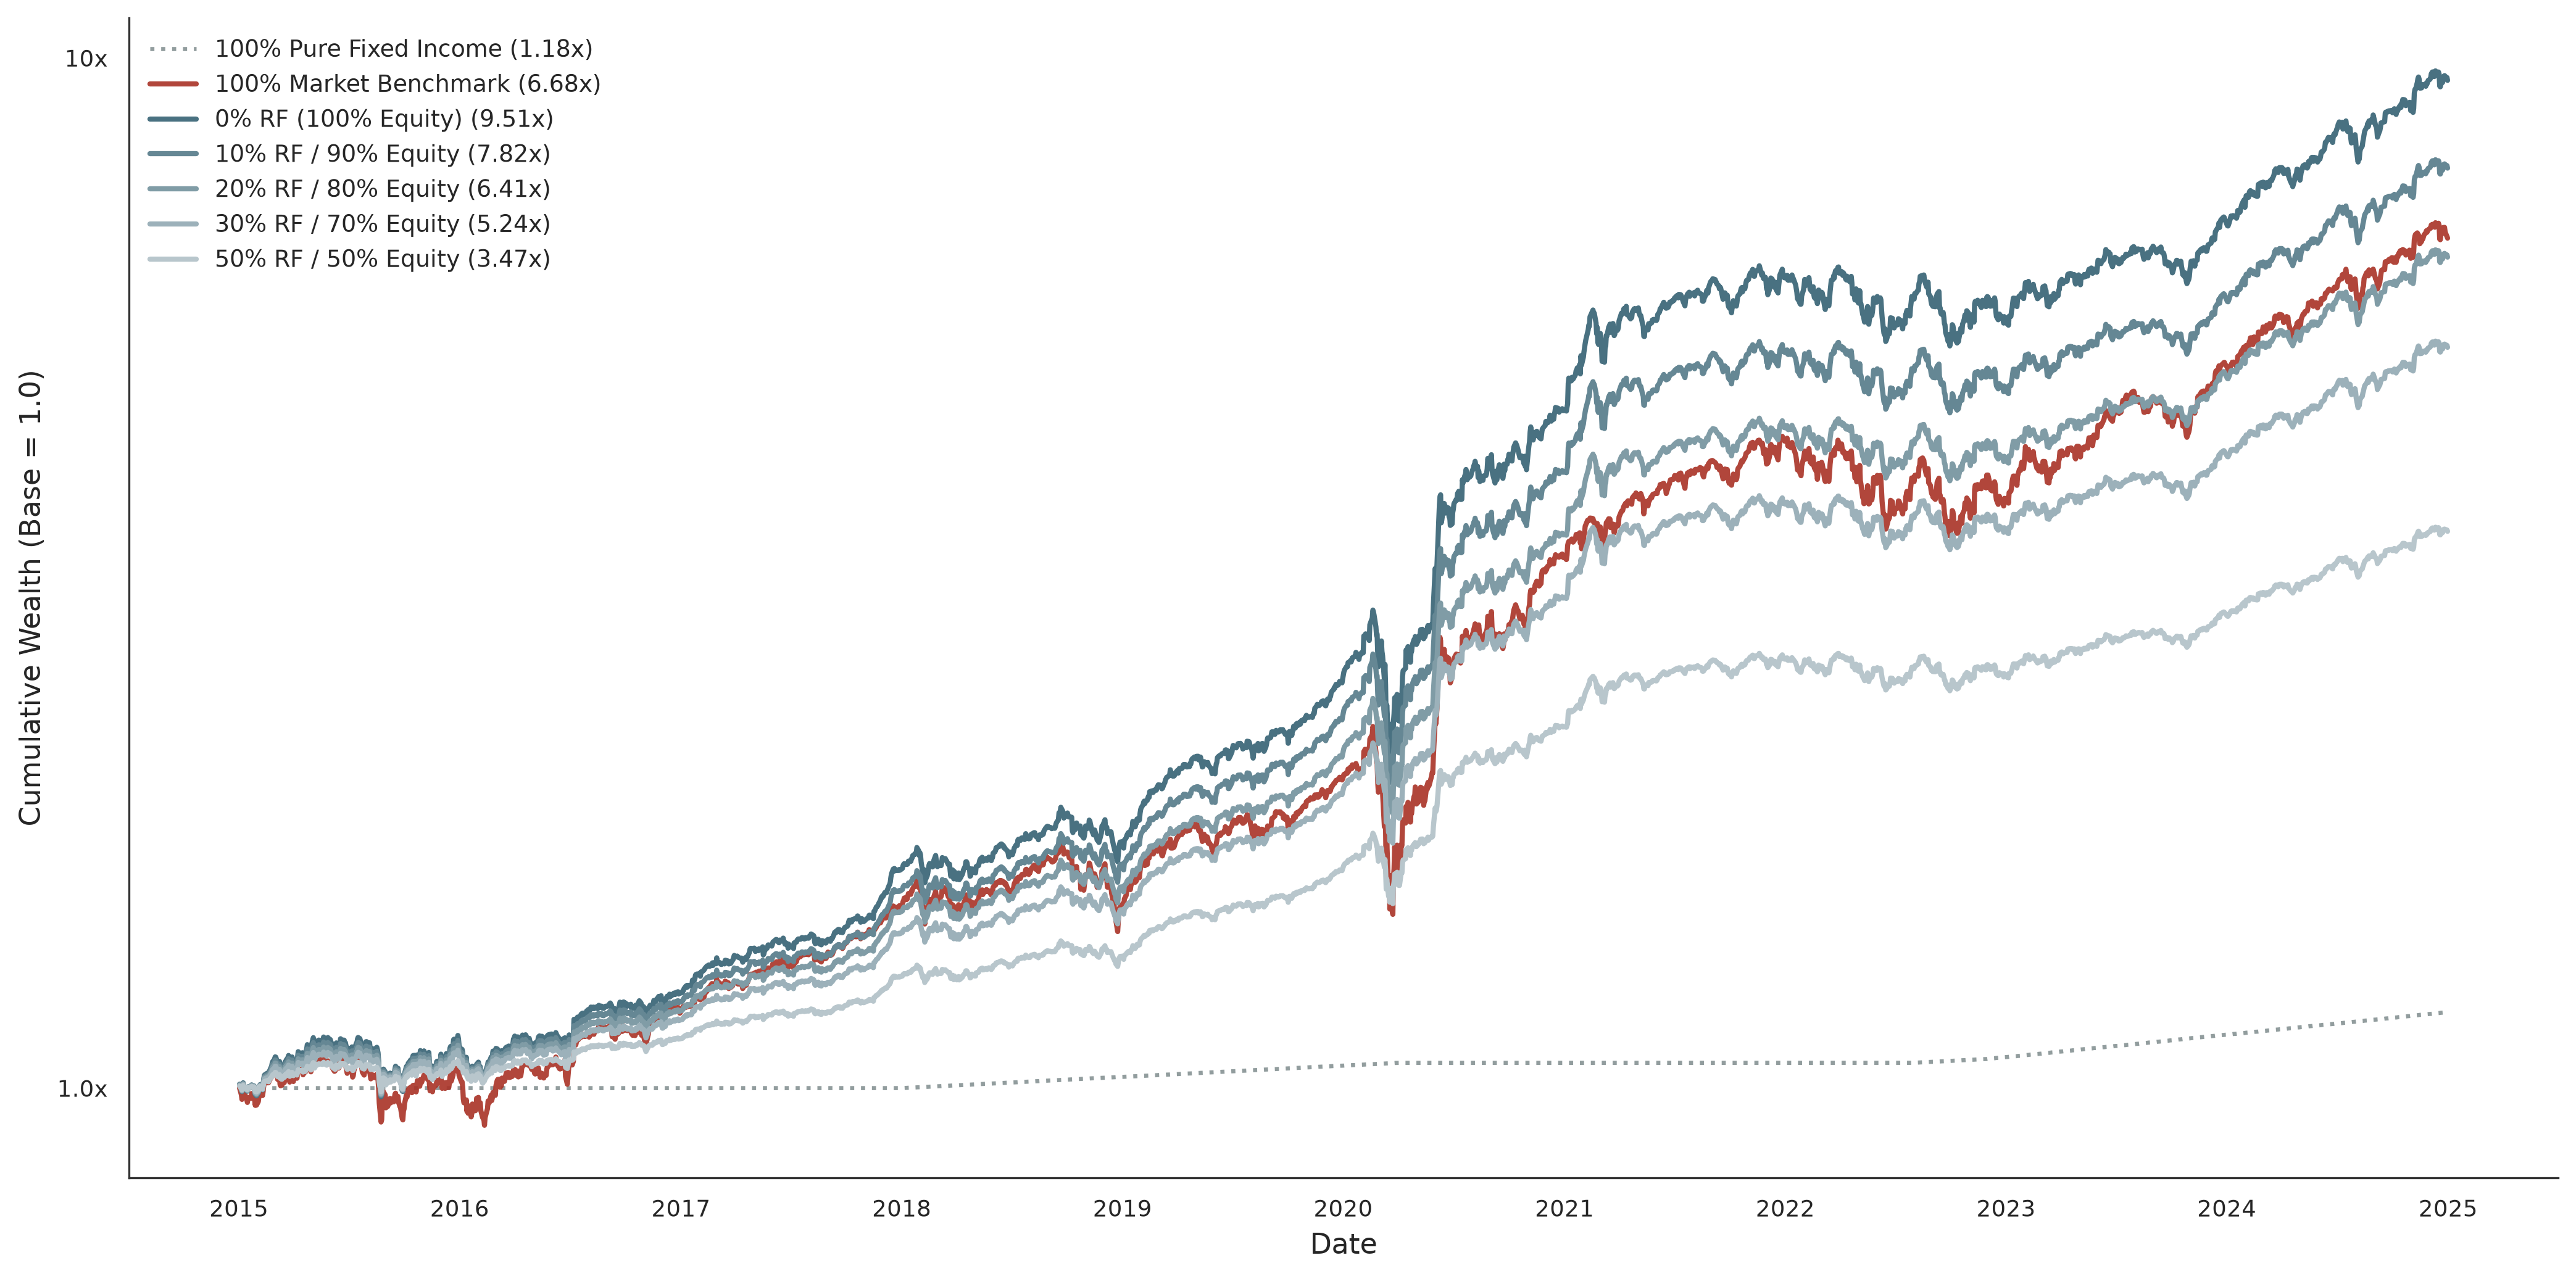
\includegraphics[width=\textwidth]{figures/hcm/13_fixed_income_blends_growth_unconstrained_hcm.png}
    \caption{Cumulative Wealth of Convex Combinations: Risk-Free Blends (HCM Unconstrained)}
    \label{fig:blends_unc_hcm}
\end{figure}

\begin{figure}[htbp]
    \centering
    \captionsetup{labelfont=normalfont, textfont=normalfont, justification=justified, singlelinecheck=off}
    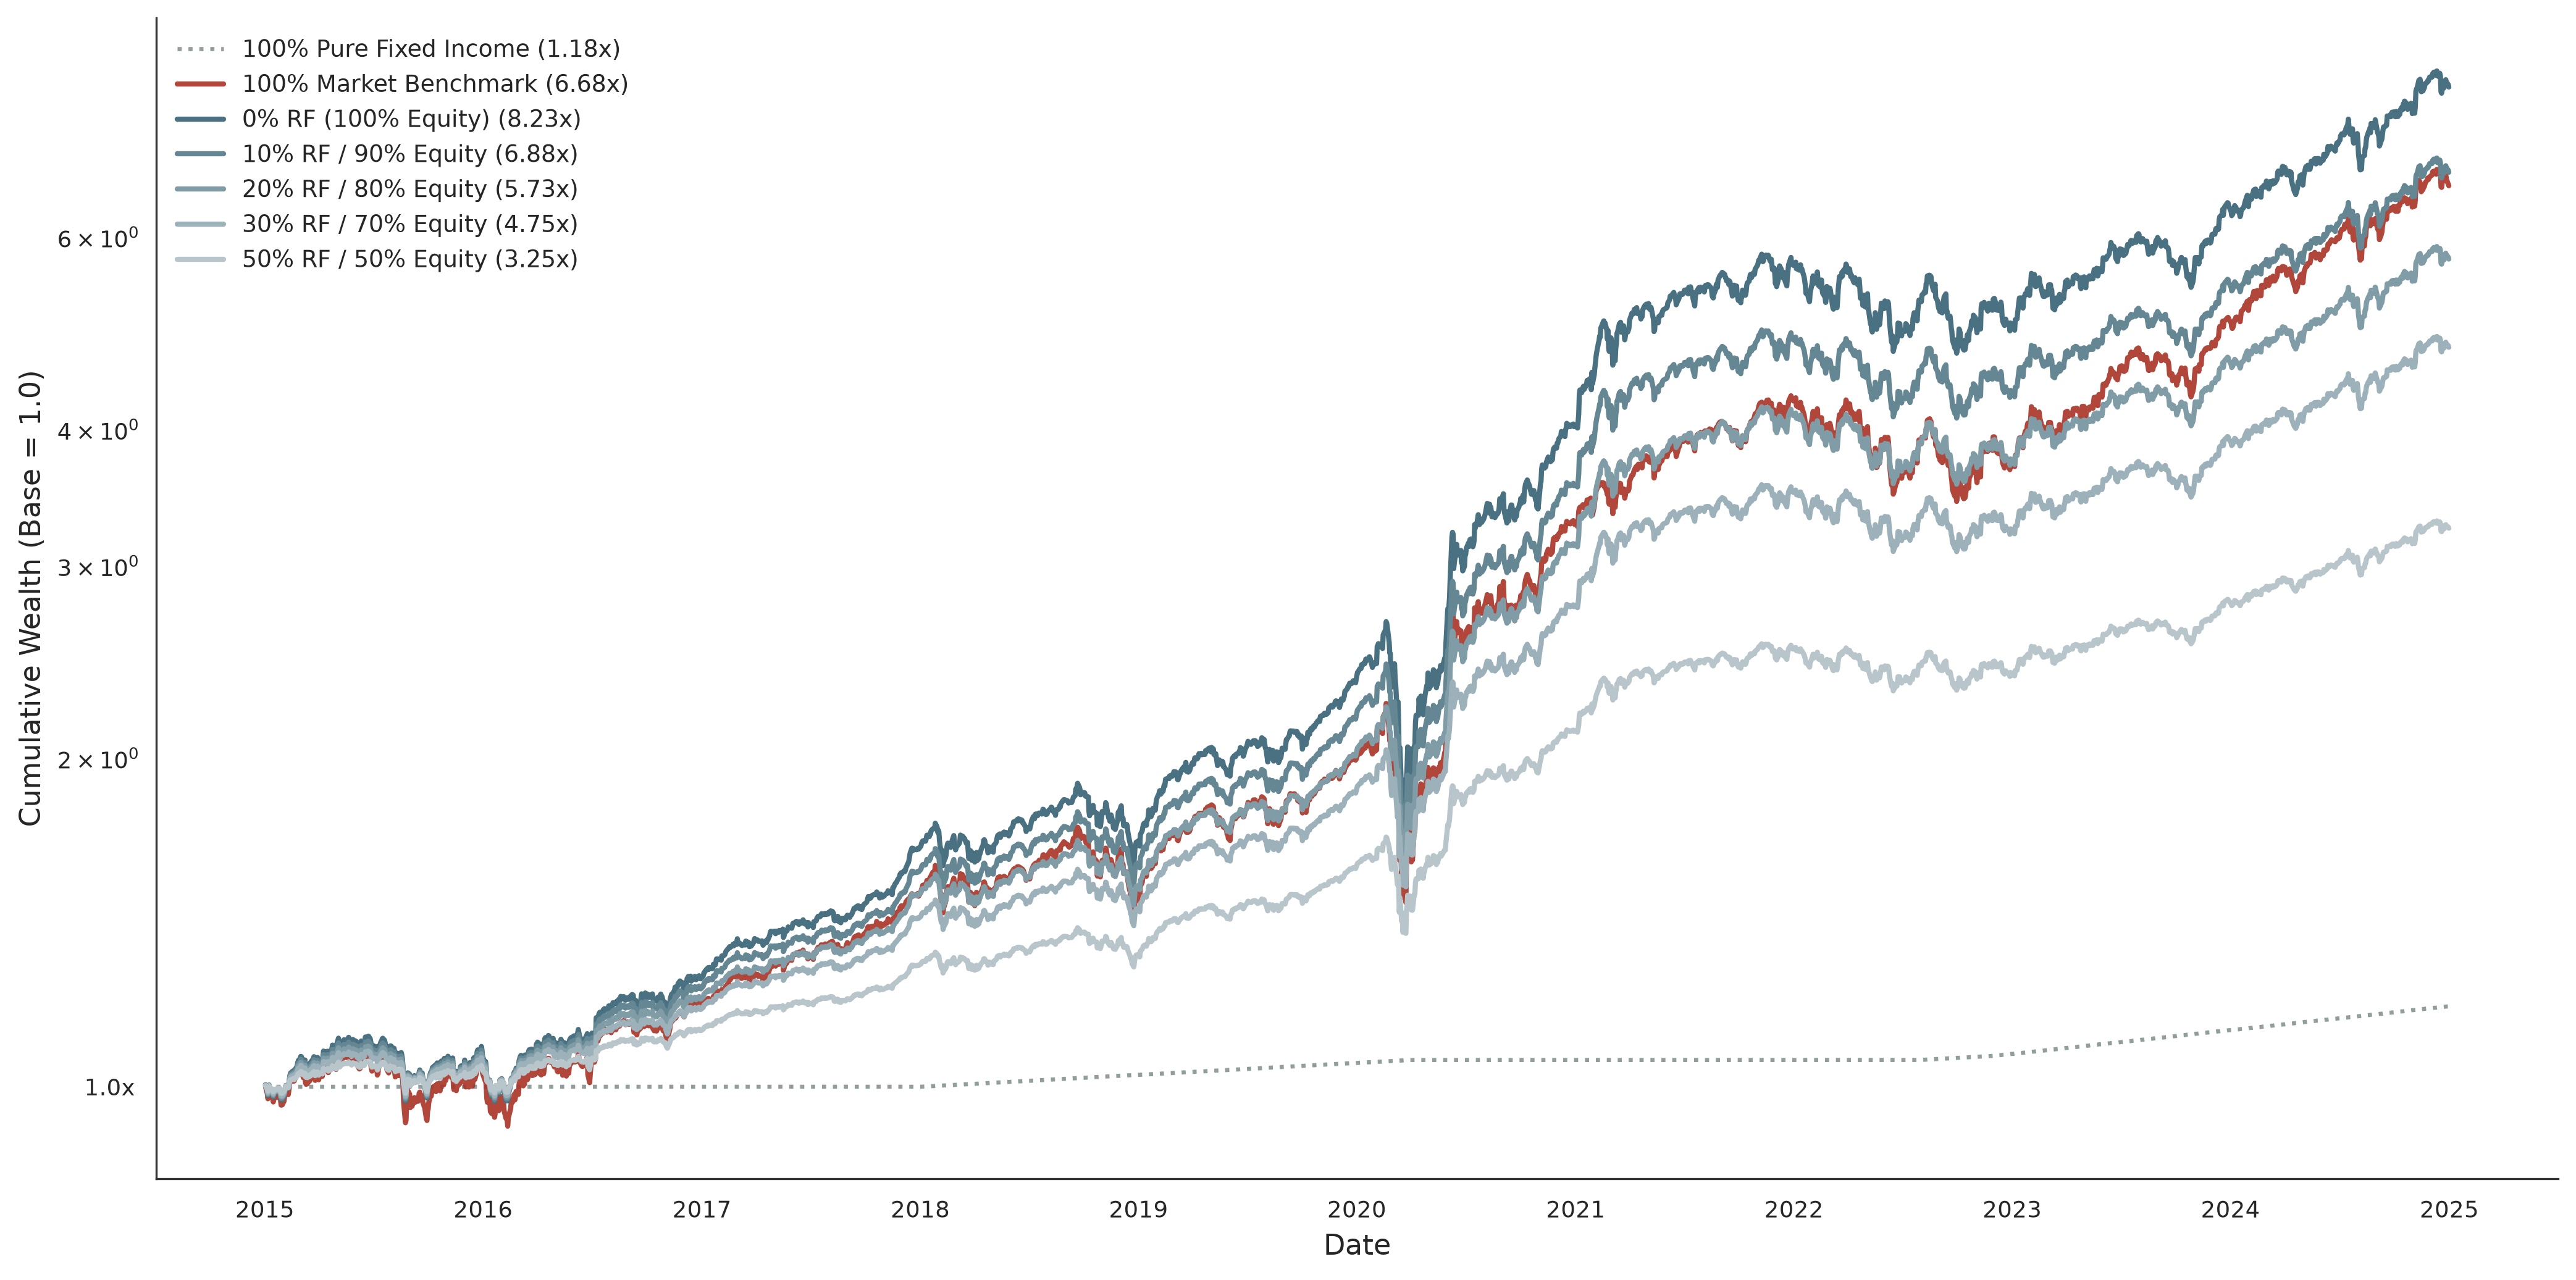
\includegraphics[width=\textwidth]{figures/hcm/14_fixed_income_blends_growth_long_only_hcm.png}
    \caption{Cumulative Wealth of Convex Combinations: Risk-Free Blends (HCM Long-Only)}
    \label{fig:blends_lo_hcm}
\end{figure}

This geometrical advantage translates into highly resilient multi-asset portfolios. For instance, blending 20\% Risk-Free Treasury Bills with 80\% of the HCM Unconstrained equity strategy generates a CAGR of 20.45\% with an annualized volatility of 13.09\%. This specific formulation virtually matches the raw returns of the 100\% Equity Benchmark (20.96\%) while stripping out over 500 basis points of annualized volatility and reducing the Maximum Drawdown from -34.28\% to -22.72\%. 

\begin{figure}[htbp]
    \centering
    \captionsetup{labelfont=normalfont, textfont=normalfont, justification=justified, singlelinecheck=off}
    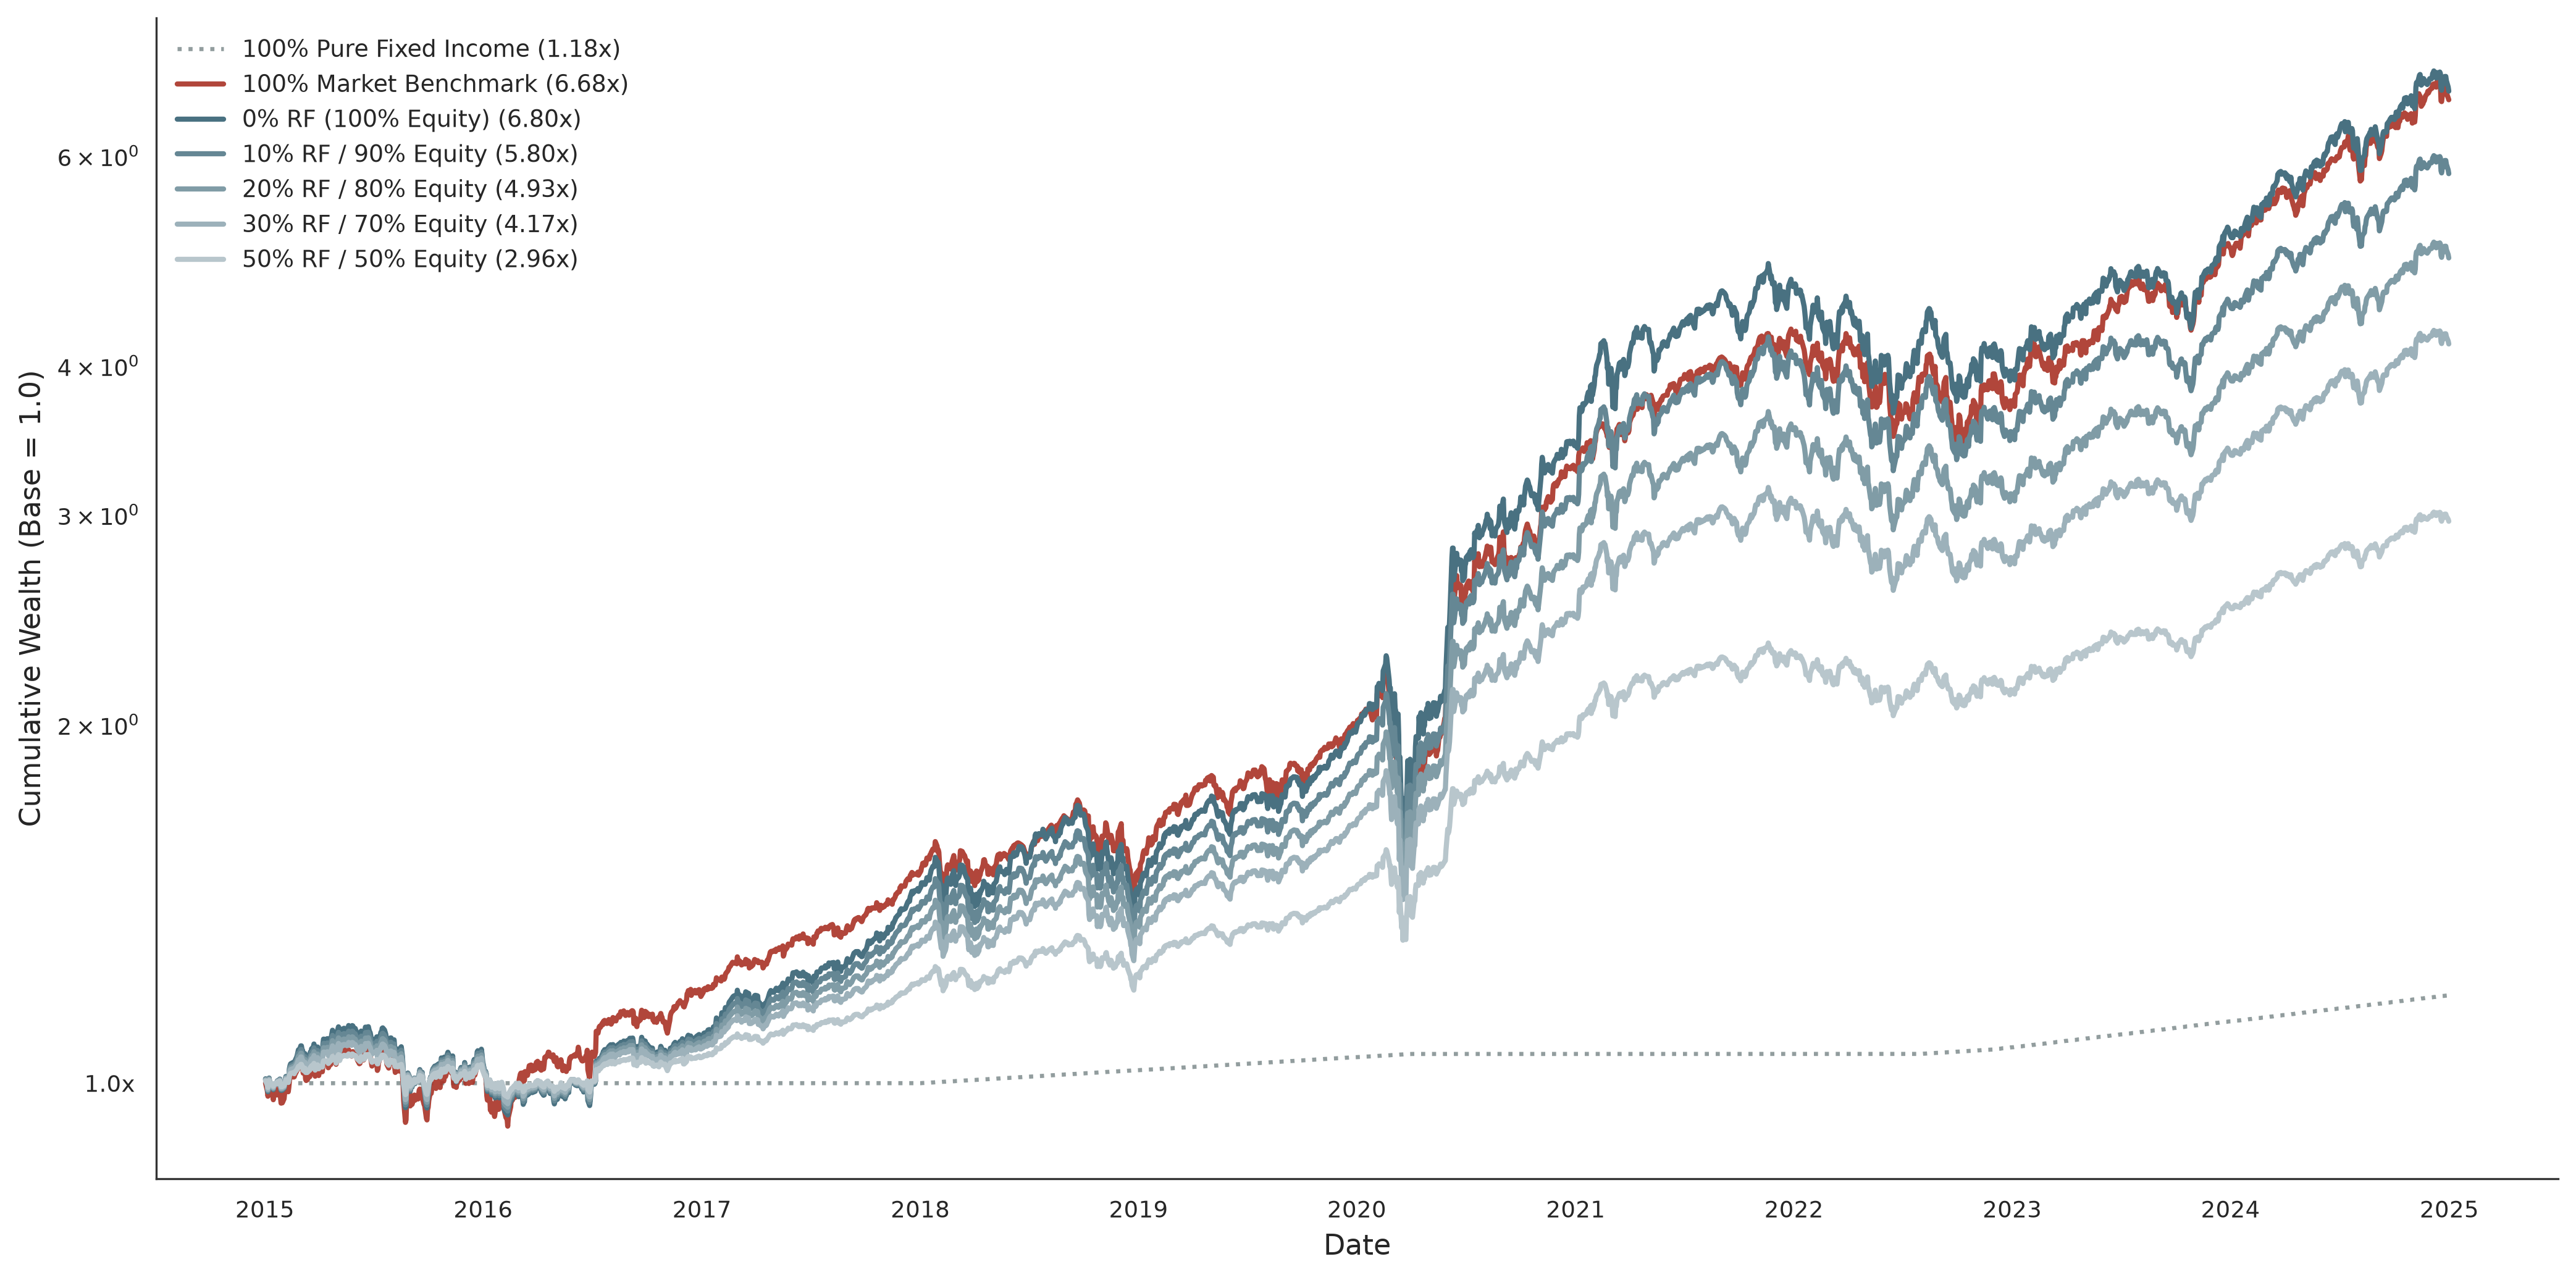
\includegraphics[width=\textwidth]{figures/pozzi/13_fixed_income_blends_growth_unconstrained_pozzi.png}
    \caption{Cumulative Wealth of Convex Combinations: Risk-Free Blends (Pozzi Unconstrained)}
    \label{fig:blends_unc_pozzi}
\end{figure}

\begin{figure}[htbp]
    \centering
    \captionsetup{labelfont=normalfont, textfont=normalfont, justification=justified, singlelinecheck=off}
    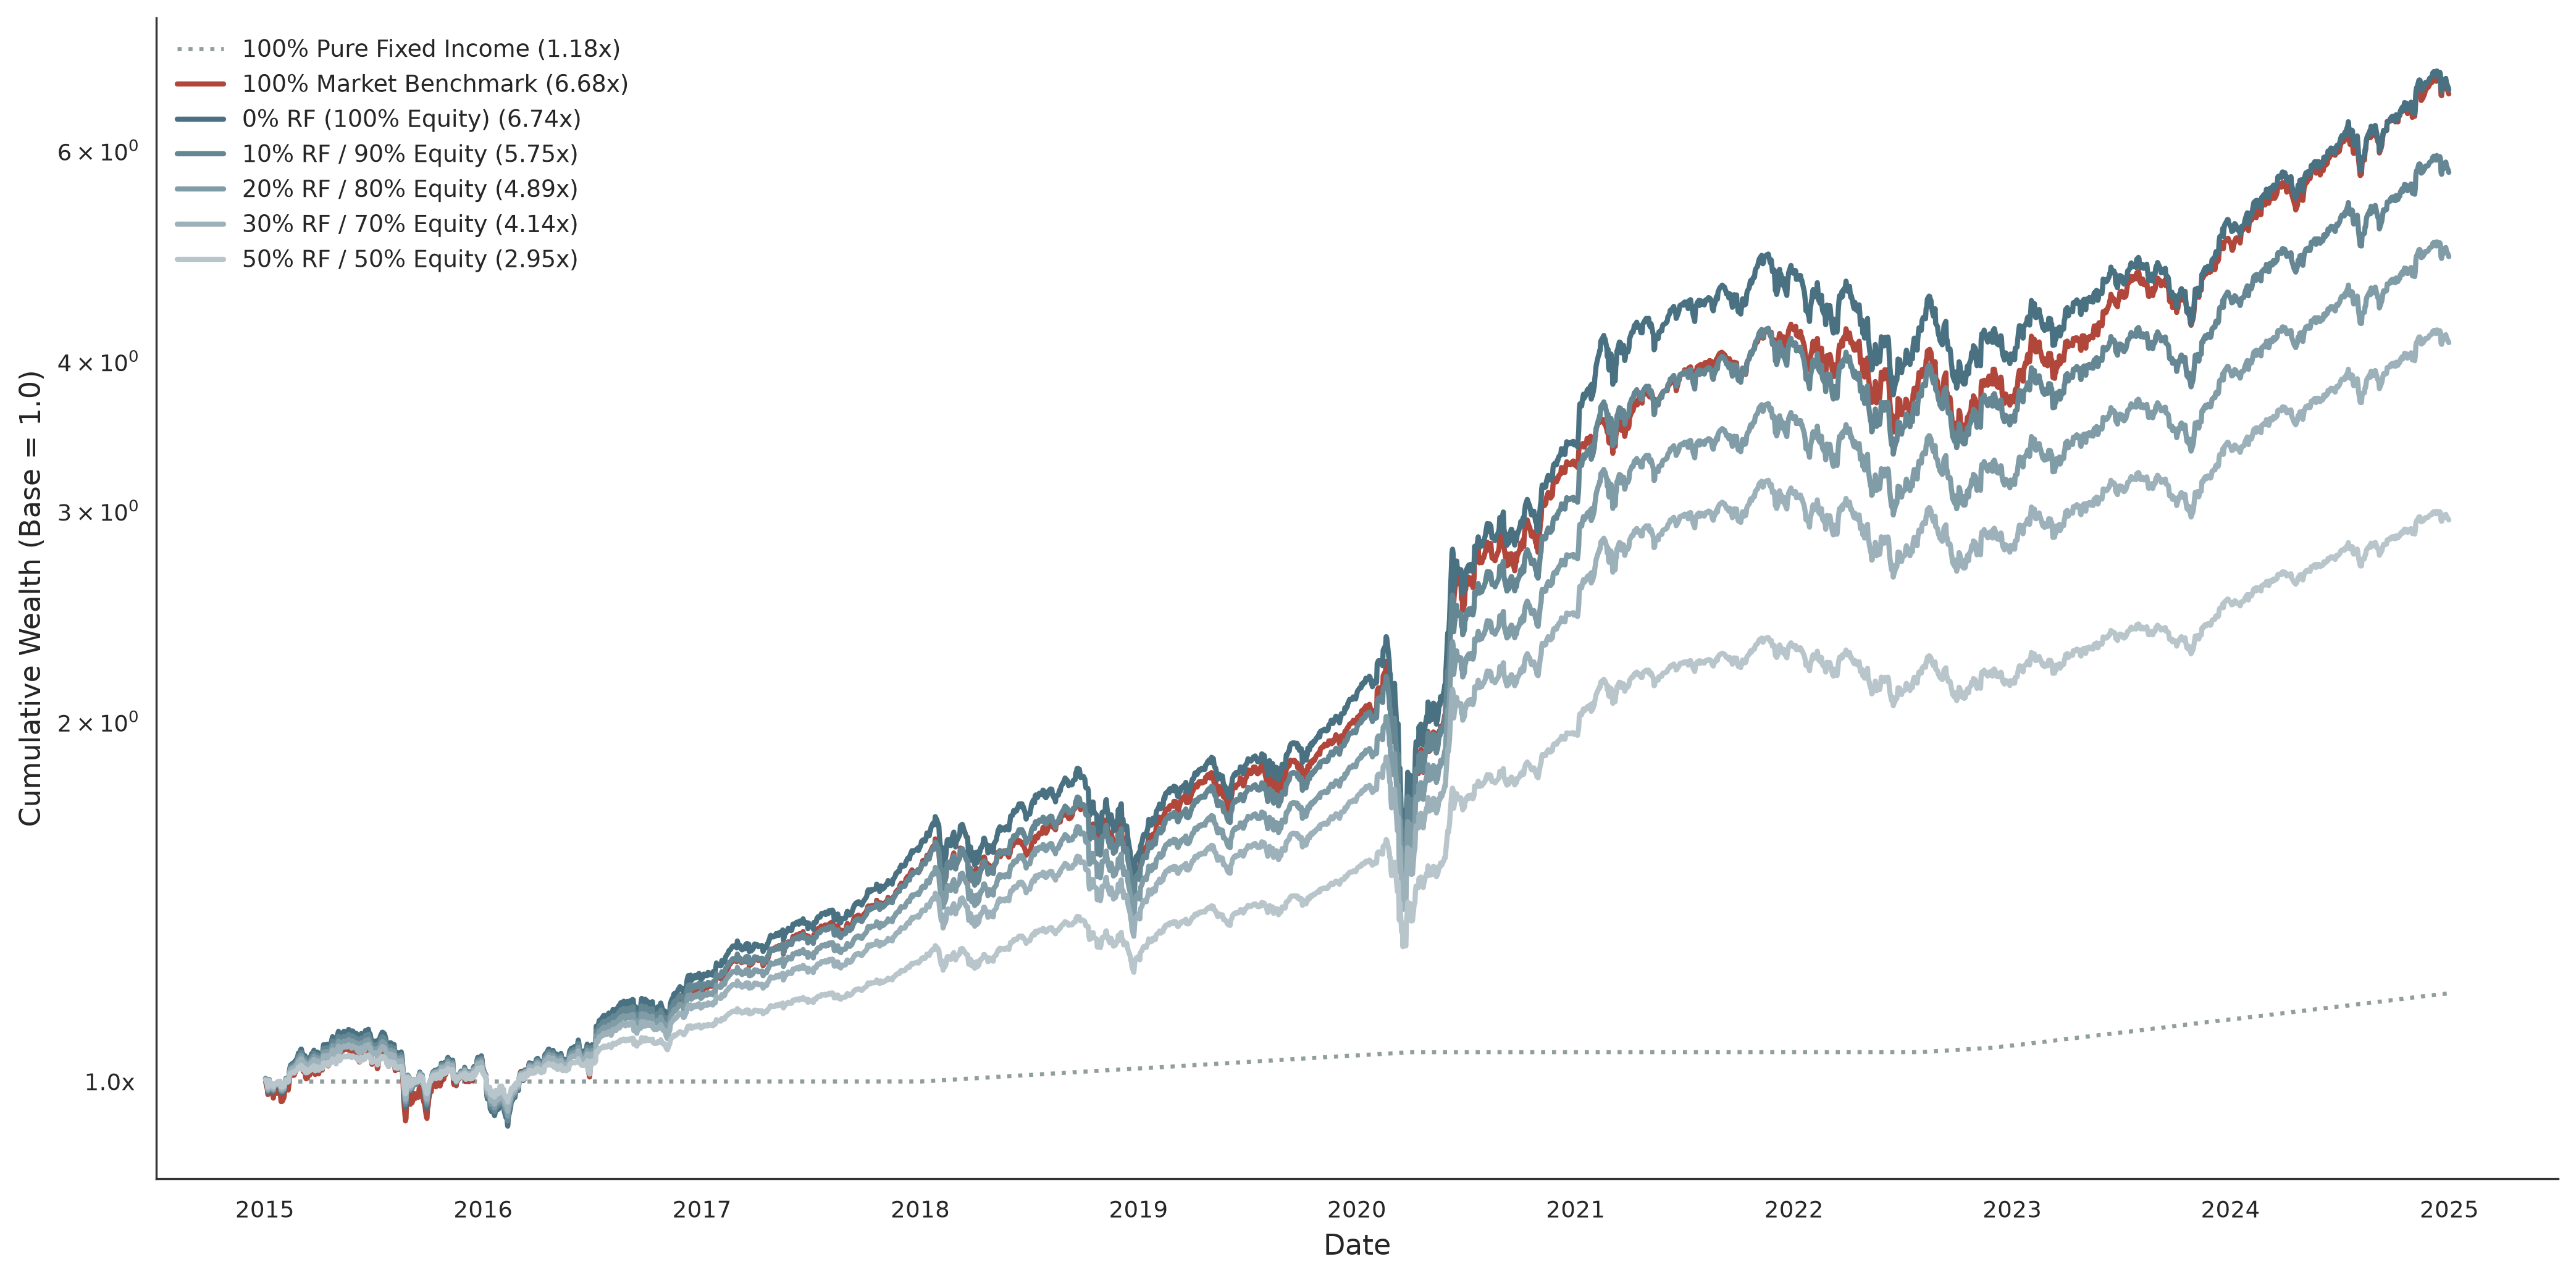
\includegraphics[width=\textwidth]{figures/pozzi/14_fixed_income_blends_growth_long_only_pozzi.png}
    \caption{Cumulative Wealth of Convex Combinations: Risk-Free Blends (Pozzi Long-Only)}
    \label{fig:blends_lo_pozzi}
\end{figure}

As depicted in Figures \ref{fig:blends_unc_pozzi} and \ref{fig:blends_lo_pozzi}, the Pozzi metric, anchored by a lower Sharpe slope of 1.04, fails to provide this same magnitude of portfolio efficiency enhancement when combined with fixed income. Ultimately, the HCM serves as a highly robust mechanism for scaling institutional wealth while systematically constraining drawdown variance.

\vskip 1em
\begin{table}[htbp]
\centering
\captionsetup{labelfont=normalfont, textfont=normalfont, justification=justified, singlelinecheck=off}
\resizebox{\textwidth}{!}{
\begin{tabular}{@{}lcccc@{}}
\toprule
Parameter & HCM Unc. & HCM LO & Pozzi Unc. & Pozzi LO\\ \midrule
\multicolumn{5}{@{}l}{\textbf{Panel A: 100\% Equity (0\% Cash)}} \\
CAGR & 25.31\% & 23.51\% & 21.16\% & 21.05\% \\
Annual Volatility & 16.36\% & 17.60\% & 18.41\% & 18.22\% \\
Sharpe Ratio & 1.36 & 1.19 & 1.04 & 1.05 \\
Max Drawdown & -27.85\% & -34.42\% & -30.50\% & -34.83\% \\ \midrule
\multicolumn{5}{@{}l}{\textbf{Panel B: 80\% Equity / 20\% Cash}} \\
CAGR & 20.45\% & 19.10\% & 17.31\% & 17.23\% \\
Annual Volatility & 13.09\% & 14.08\% & 14.72\% & 14.58\% \\
Sharpe Ratio & 1.36 & 1.19 & 1.04 & 1.05 \\
Max Drawdown & -22.72\% & -28.30\% & -24.93\% & -28.66\% \\ \midrule
\multicolumn{5}{@{}l}{\textbf{Panel C: 60\% Equity / 40\% Cash}} \\
CAGR & 15.65\% & 14.71\% & 13.43\% & 13.37\% \\
Annual Volatility & 9.81\% & 10.56\% & 11.04\% & 10.93\% \\
Sharpe Ratio & 1.36 & 1.19 & 1.04 & 1.05 \\
Max Drawdown & -17.34\% & -21.79\% & -19.08\% & -22.07\% \\ \midrule
\end{tabular}}
\vskip 1em
\caption{Capital Allocation Line \& Cash Convex Combinations Comparison}
\label{tab:cal_blends}
\end{table}

\subsection{Robustness and Limitations}\label{sec:robustness}

\noindent\textbf{Orthogonality of HCM to standard characteristics.} A natural concern is that HCM may merely repackage well-known firm characteristics. To address this, we regress, for each estimation window, the cross-sectional HCM score on market beta, log market capitalization, and twelve-month momentum. The pooled explanatory power is modest: the average $R^2$ across the 2015--2024 windows is $0.3829$, ranging from $0.2668$ (2024) to $0.5887$ (2018). Roughly 62\% of the cross-sectional variation in HCM is therefore orthogonal to these standard characteristics, supporting its interpretation as a distinct topological dimension. At the same time, the metric is clearly not independent of firm size, and the test does not include illiquidity measures; a spanning analysis against a true illiquidity factor \citep{amihud2002illiquidity} remains an important extension, which we complement below with size and low-risk spanning tests.

\noindent\textbf{Multiple testing and regime dependence.} Table~\ref{tab:robustness} summarizes the robustness of the peripheral (Decile~10) portfolio across the specifications below. We first ask whether the peripheral alpha survives corrections for multiplicity \citep{harvey2016and}. Pooled across the out-of-sample sample, the Decile~10 FF3 alpha is $0.101$ per annum ($t=2.93$); its Holm--Bonferroni adjusted $p$-value across the ten deciles is $0.034$, and a White reality-check block bootstrap yields $p=0.006$. The premium is therefore not an artefact of searching across deciles. It is, however, regime-dependent: the alpha is $0.206$ ($t=2.77$) over 2015--2019 but statistically indistinguishable from zero ($0.014$, $t=0.27$) over 2020--2024, while the core's negative alpha is concentrated in the second half ($-0.037$, $t=-3.41$).

\noindent\textbf{Size and low-risk spanning.} To test whether the peripheral premium is simply a small-cap or low-beta effect, we first form a size double sort: within each year and each market-capitalization tercile we re-sort the universe by HCM and retain the extreme deciles. The peripheral alpha is concentrated in the small-cap tercile ($0.143$, $t=2.47$) and is statistically indistinguishable from zero in the mid- ($0.018$, $t=0.57$) and large-cap ($-0.008$, $t=-0.36$) terciles. We then add a betting-against-beta (BAB) factor \citep{frazzini2014betting} to the FF3 regression. The peripheral alpha falls modestly, from $0.087$ ($t=2.81$) to $0.076$ ($t=2.63$), with a significantly positive BAB loading of $0.347$ ($t=7.35$). The peripheral premium thus retains an independent component but is partly a low-beta phenomenon and is not present among large caps.

\noindent\textbf{Stocks-only replication.} Because the core is heavily populated by exchange-traded funds after 2017, we rebuild the networks on individual stocks only. Re-estimating the correlation matrices and TMFG on the stock universe, the peripheral alpha declines from $0.101$ to $0.048$ ($t=2.74$) and the peripheral market beta rises from $0.281$ to $0.718$; the core's negative alpha disappears ($0.093$, $t=1.66$). A faster variant that induces the stock subgraph on the existing network gives a similar picture ($0.028$, $t=1.97$; $\beta=0.746$). The clean core--periphery separation documented above is therefore amplified by non-stock vehicles, which track broad indices by construction.

\noindent\textbf{Costs and capacity.} Re-pricing the extreme portfolios under liquidity-conditioned costs barely changes the net performance: with the peripheral turnover of $45.7\%$ per year, the Decile~10 CAGR moves from $15.24\%$ (gross) to $15.20\%$ (flat 10 bps) and $14.89\%$ (liquidity-tiered), and the D1\&D10 combination from $12.08\%$ to $11.71\%$. For the concentrated top-25 periphery holdings, under a square-root market-impact law with a daily ADV proxy of roughly \$12bn, net alpha decays gradually, from $0.100$ at \$1m to $0.088$ at \$1bn and $0.059$ at \$10bn. These figures are conditional on the assumed impact coefficient and turnover velocity; with the concentrated holdings, capacity would decline faster, and the estimates should be re-estimated with observed dollar volume before any capacity claim is made.

\noindent\textbf{Limitations.} Several caveats qualify our findings. First, the \emph{out-of-sample lead--lag} advantage of the network hierarchy does not survive: once projected beyond the estimation window, the traditional size effect is the more resilient predictor and the network signal occasionally turns negative; the strong in-sample result should be read as descriptive of the estimation window. Second, the \emph{universe construction} is not point-in-time in the sense of a delisting-aware constituent file, so a survivorship bias cannot be fully ruled out. Third, the \emph{peripheral premium} is concentrated in small caps and before 2020 and is partly explained by the low-beta (BAB) effect; a spanning test against a true illiquidity factor \citep{amihud2002illiquidity} awaits dollar-volume data. Fourth, the \emph{cost and capacity} numbers rely on assumed impact parameters. Finally, the lead--lag signal peaks around 2020, reinforcing the regime dependence documented above.

\begin{table}[!htbp]
    \caption{Robustness of the HCM peripheral (Decile~10) portfolio. All alphas are annualized; the baseline row is the published in-sample-network specification, the remaining rows are out-of-sample re-estimations. The pooled OOS alpha survives Holm--Bonferroni ($p=0.034$) and reality-check ($p=0.006$) corrections but is concentrated in small caps and in the first half of the sample, is partly explained by a betting-against-beta factor, and weakens once non-stock vehicles are excluded.}
    \label{tab:robustness}
    \centering
    \begin{tabular}{lccc}
    \toprule
    Specification & Peripheral $\alpha$ (p.a.) & $t$-stat & Mkt $\beta$ \\
    \midrule
    Baseline (published)          & 0.101 & 2.07 & 0.281 \\
    Pooled OOS                    & 0.101 & 2.93 & 0.334 \\
    \quad 2015--2019              & 0.206 & 2.77 & 0.198 \\
    \quad 2020--2024              & 0.014 & 0.27 & 0.378 \\
    Stocks-only (rebuild)         & 0.048 & 2.74 & 0.718 \\
    Small-cap tercile             & 0.143 & 2.47 & 0.265 \\
    Large-cap tercile             & $-0.008$ & $-0.36$ & 0.384 \\
    FF3 $+$ BAB                   & 0.076 & 2.63 & --- \\
    \bottomrule
    \end{tabular}
\end{table}

\section{Conclusion}\label{sec:conclusion}

\noindent This paper examines the structural topology of the equity market, demonstrating that network-based centrality metrics translate complex cross-asset dependencies into actionable asset pricing and portfolio management frameworks. By evaluating the Hybrid Centrality Metric (HCM) against the Pozzi metric across characteristics, risk exposures, information diffusion, and out-of-sample performance, we show that the choice of topological filter dictates the economic value of the resulting network. 

Our comparative analysis indicates that the HCM framework provides a remarkably stable market hierarchy. While the Pozzi metric exhibits high turnover rates and unstable risk profiles, the HCM isolates a persistent market structure. At the core of this hierarchy lie large-cap equities deeply integrated with systematic market factors. As evidenced by our lead--lag analysis, these central assets act as primary informational conduits, rapidly reflecting macroeconomic shocks and systematically leading the broader network in sample; out of sample, as discussed above, this lead--lag advantage weakens relative to the size effect.

Conversely, the network's periphery represents a domain of idiosyncratic behavior. Structurally disconnected from the core, peripheral assets exhibit substantially lower systematic risk and a delayed reaction to market-wide information. This delayed processing is associated with a positive alpha that traditional risk factors do not fully span, though---as our robustness analysis shows---the effect is concentrated in small caps and is partly attributable to size and low-beta exposures. We therefore interpret HCM as a descriptive topological dimension rather than the fundamental driver of the premium itself.

To operationalize these structural insights, we deployed a quantitative portfolio optimization framework based on the Treynor-Black (1973) model. By actively weighting peripheral assets with positive alpha and systematically hedging against the highly integrated, negative-alpha central core, we constructed institutional-grade portfolios designed to efficiently harvest topological inefficiencies. Evaluated out-of-sample and strictly net of dynamic rebalancing transaction costs, the unconstrained HCM strategy delivers superior risk-adjusted performance, suppressing volatility and significantly minimizing maximum drawdowns relative to the capitalization-weighted market benchmark. 

Crucially, our Fama-French 3-factor attributions show that this outperformance is not spanned by standard market, size, or value risks---yielding over 12\% annualized in the unconstrained HCM framework---while Section~\ref{sec:robustness} documents that it is partly related to size and low-beta exposures. Furthermore, projecting these active strategies along the Capital Allocation Line (CAL) demonstrates that the HCM topology systematically shifts the efficient frontier outward. Blending this topological equity strategy with risk-free assets yields highly resilient multi-asset portfolios that drastically reduce systematic drawdowns while successfully maintaining benchmark-equivalent returns.

Ultimately, these findings suggest that correlation network topology provides a useful map of market microstructure and risk distribution. Leveraging stable methodologies such as the HCM to isolate topological extremes offers a mathematically transparent dimension for institutional risk management and alpha generation. At the same time, the out-of-sample degradation of the lead--lag signal and the metric's residual correlation with firm size indicate that network position is better understood as a structural complement to---rather than a substitute for---traditional characteristics, and future work should establish its independent pricing role through formal spanning tests. Our robustness analysis further shows that the peripheral premium, though statistically robust to multiplicity corrections, is concentrated in small caps and is partly a low-beta effect, and that the core--periphery separation is amplified by exchange-traded funds; disentangling these components is a priority for future work.

\newpage
%%%%%%%%%%%%%%%%%%%%%%%%%%%%%%%%%%%%
% REFERENCES
%%%%%%%%%%%%%%%%%%%%%%%%%%%%%%%%%%%%
\bibliography{references.bib}\label{refs}
\bibliographystyle{dcu-rbfin}
%%%%%%%%%%%%%%%%%%%%%%%%%%%%%%%%%%%%
% END OF REFERENCES
%%%%%%%%%%%%%%%%%%%%%%%%%%%%%%%%%%%%



% ==========================================
% REFERENCES
% ==========================================


















%%%%%%%%%%%%%%%%%%%%%%%%%%%%%%%%%%%%

%%%%%%%%%%%%%%%%%%%%%%%%%%%%%%%%%%%%
% APPENDIX
%%%%%%%%%%%%%%%%%%%%%%%%%%%%%%%%%%%%


\end{document}

%%%%%%%%%%%%%%%%%%%%%%%%%%%%%%%%%%%%
% END OF DOCUMENT
%%%%%%%%%%%%%%%%%%%%%%%%%%%%%%%%%%%%